In this chapter, the results of various experiments conducted to investigate \ac{ap} axis alignment in \ac{ce} embryo are reported, along with their comparison to the numerical simulations of the theoretical model of \ac{ap} axis alignment described in \autoref{sec:apAxisAlignmentModelMN}. This chapter follows \citep{axisConvergence} closely. Experiments described here were performed in collaboration with Peter Gross and Mirna Kramer from Technische Universit{\"a}t Dresden; with numerical simulations by Michael Nestler from Technische Universit{\"a}t Dresden.

\begin{table}
    \centering
    \begin{tabular}{|C{0.3\textwidth}|C{0.3\textwidth}|C{0.3\textwidth}|}
        \hline
        Experimental Condition & Strain & No. of Embryos\\
        \hline
        Unperturbed & SWG070 & \num{57}\\
        \geneExp{mlc-4} \ac{rnai} & SWG070 & \num{10}\\
        \geneExp{nop-1} \ac{rnai} & SWG070 & \num{9}\\
        \geneExp{nop-1; mel-11} \ac{rnai} & SWG070 & \num{69}\\
        \geneExp{ima-3} \ac{rnai} & SWG070 & \num{35}\\
        \geneExp{air-1} \ac{rnai} & SWG070 & \num{23}\\
        \geneExp{air-1; mel-11} \ac{rnai} & SWG228 & \num{13}\\
        Unperturbed & SWG057 & \num{32}\\
        \geneExp{goa-1; gpa-16} \ac{rnai} & SWG057 & \num{30}\\
        \hline
    \end{tabular}
    \caption{Number of embryos in various experimental conditions described in this chapter.}
    \label{tab:resultsNumberEmbryo}
\end{table}

\section{Characterising \acs{ap} axis alignment in unperturbed embryos} \label{sec:apAxisAlignCharacteriseWT}
\ac{ap} axis alignment is first characterised in unperturbed embryos. \enquote{Unperturbed} here refers to no genetic perturbations, such as no \ac{rnai} or mutations, apart from the addition of fluorescent tags. To this end, time-lapse microscopy of embryos from the SWG070 strain was undertaken, which is labelled with \flurophoreLabel{\ac{nmy2}}{\ac{gfp}} and \flurophoreLabel{phDomain}{mCherry} -- as described in \autoref{sec:microscope}. In these embryos, the male pronucleus can be observed as a dark circle in the cytoplasm, in the \flurophoreLabel{\ac{nmy2}}{\ac{gfp}} fluorescent channel -- as cytoplasmic myosin is excluded from the proncleus. The posterior domain as the depletion of \ac{nmy2} on the cortex near the male pronucleus. The \ac{ap} axis alignment process is characterised by tracking the position of the male pronucleus as it undergoes posteriorisation. See \autoref{sec:imageAnalysis} for details on the image analysis methods used to track the male pronucleus. 

\begin{figure}
\centering
\includegraphics[width=\textwidth]{Results/FigExpUnperturbed/wtMicrograph.pdf}
\caption[Representative micrograph: Unperturbed embryos]{Representative unperturbed embryo of SWG070 strain, labelled with \flurophoreLabel{\ac{nmy2}}{\ac{gfp}} (white), showing the posteriorisation of the male pronucleus and the concurrent movement of the myosin depletion (indicating the \ac{ppar} domain) towards the posterior end. The male pronucleus can be visualized as the dark circle in the myosin channel towards the posterior end (right). t = \SI{0}{\second} is set at the end of posteriorisation of the male pronucleus. Scale bar: \SI{10}{\unitLength}. Images are rotated such that anterior and posterior ends are to the left and right respectively.}
\label{fig:swg070WtMicrograph}
\end{figure}

Two aspects of the posteriorisation of the male pronucleus are quantified: its \enquote{angular position} and \enquote{posteriorisation velocity} (see \autoref{sec:imageAnalysis}). Angular position refers to the angle made between the long axis and the line connecting the center of the male pronucleus to the center of the embryo. Posteriorisation velocity is the component of the velocity of the male pronucleus that is parallel to the cortex (at the given angular position). Negative posteriorisation velocities indicate movement in direction of decreasing angular positions and thus towards the posterior end, positive posteriorisation velocity in direction of increasing angular positions and thus away from the posterior end. End of posteriorisation is denoted as the zero time-point (t = \SI{0}{\second}), and all movies are synchronised using this time-point. 

Plotting the angular position as a function of time, the angular positions were found to generally decrease towards \SI{0}{\unitAngle} as time reaches closer to end of posteriorisation (t = \SI{0}{\second}). Specifically, in embryos where the \ac{ap} axis is mis-aligned -- that is, with initial angular position greater than \SI{5}{\unitAngle} (\num{33} out of \num{57} embryos) -- the \ac{ap} axis re-aligns back towards the long axis. Furthermore, this decay towards \SI{0}{\unitAngle} was quantified by fitting an exponential $\alpha = \alpha_0 + \exp(-\frac{t}{t_0})$ to the plotted angular positions, yielding a time constant $t_0 = \SI{119 +- 3}{\second}$ and $\alpha_0 = \SI{-0.75 +- 0.3}{\unitAngle}$. These observations confirm those made in \cite{goldstein1996specification} -- the \ac{ap} axis does align itself towards the long axis of the embryo, evidenced by the posteriorisation of the male pronucleus. Note that the exponential fit considered here is only phenomenological, and does not attempt to capture any physically relevant features of \ac{ap} axis alignment -- rather it allows for easier comparison of the decreasing angular positions in different experimental conditions considered in this chapter.

\begin{figure}
\centering
\begin{subfigure}[t]{0.4\textwidth}
    \centering
    \includegraphics[width=\textwidth]{Results/FigExpUnperturbed/wtTrajectories.pdf}
    \caption{Trajectories of the male pronucleus (denoted by the coordinates of its center) observed in unperturbed embryos. Color represents time. x- and y-axes lie along the long and short axes of an ellipse with semi-major axis $a = \SI{28.9}{\unitLength}$ and semi-minor axis $b = \SI{16.3}{\unitLength}$. Scale bar: \SI{5}{\unitLength}} 
    \label{subfig:swg070WtTrajectories-tracks}
\end{subfigure}
\hfill
\begin{subfigure}[t]{0.57\textwidth}
    \centering
    \includegraphics[width=\textwidth]{Results/FigExpUnperturbed/wtAngular.pdf}
    \caption{Angular position of the male pronucleus (on y-axis, in \si{\unitAngle}) plotted as a function of time (on x-axis, in \si{\second}), in unperturbed embryos. Thin grey lines represent individual trajectories, thick black line represents a exponential fit to the average of these tracks: $\alpha = \alpha_0 + \exp(-\frac{t}{t_0})$, with $t_0 = \SI{119 +- 3}{\second}$ and $\alpha_0 = \SI{-0.75 +- 0.3}{\unitAngle}$.} 
    \label{subfig:swg070WtTrajectories-angleVsTime}
\end{subfigure}
\caption[Experimentally observed trajectories of the male pronucleus in unperturbed embryos]{Experimentally observed trajectories of the male pronucleus during posteriorisation in unperturbed embryos of SWG070 strain (N = 57). See \autoref{subsec:nucleusTracking} for details on male pronucleus tracking. Average semi-major and semi-minor axes lengths for unperturbed embryos of SWG070 strain are used in \autoref{subfig:swg070WtTrajectories-tracks} -- see \autoref{tab:resultsEmbryoGeometry}. Angular position is defined as the angle between the long axis and line connecting the centers of the male pronucleus and embryo, depicted in \autoref{subfig:swg070WtTrajectories-tracks}. t = \SI{0}{\second} denotes end of posteriorisation.}
\label{fig:swg070WtTrajectories}
\end{figure}

Plotting the posteriorisation velocity as a function of angular position (see \autoref{sec:statAnalysis} for details on binning of angular positions), it is found that the male pronucleus is, on average, moving towards the posterior end (as indicated by the negative sign of the velocity) -- with higher speed at higher angular positions (\autoref{fig:swg070WtPostVelVsAngle}). This can also be observed as increasing magnitude of slope of the angular position vs time plots for higher angular positions in \autoref{subfig:swg070WtTrajectories-angleVsTime}. Based on this observation, it is concluded here that the rate of \ac{ap} axis alignment is faster at higher angular positions: the male pronucleus moves faster towards the posterior end the further away from the posterior end it is.

\begin{table}
    \centering
    \begin{tabular}{|C{0.2\textwidth}|C{0.55\textwidth}|C{0.2\textwidth}|}
        \hline
        Angular positions (\si{\unitAngle}) & Posteriorisation velocity (\SI{1e-1}{\unitPostVel}) & No. of embryos\\
        \hline
        \numrange{0}{3} & \num{-0.15} (\num{-0.18},\num{-0.13}) & 37\\
        \numrange{3}{6} & \num{-0.17} (\num{-0.20},\num{-0.14}) & 36\\
        \numrange{6}{9} & \num{-0.27} (\num{-0.30},\num{-0.23}) & 31\\
        \numrange{9}{12} & \num{-0.40} (\num{-0.46},\num{-0.35}) & 27\\
        \numrange{12}{15} & \num{-0.46} (\num{-0.52},\num{-0.41}) & 20\\
        \numrange{15}{18} & \num{-0.40} (\num{-0.47},\num{-0.34}) & 16\\
        \numrange{18}{21} & \num{-0.49} (\num{-0.58},\num{-0.40}) & 13\\
        \numrange{21}{24} & \num{-0.85} (\num{-0.98},\num{-0.72}) & 10\\
        \numrange{24}{27} & \num{-1.12} (\num{-1.26},\num{-0.97}) & 8\\
        \hline
    \end{tabular}
    \caption{Posteriorisation velocity measured for each angular position bin in unperturbed embryos. Average posteriorisation velocity along with \num{95}\% confidence interval for the average are reported.}
    \label{tab:resultsPostVelUnperturbed}
\end{table}

\begin{figure}[p]
\centering
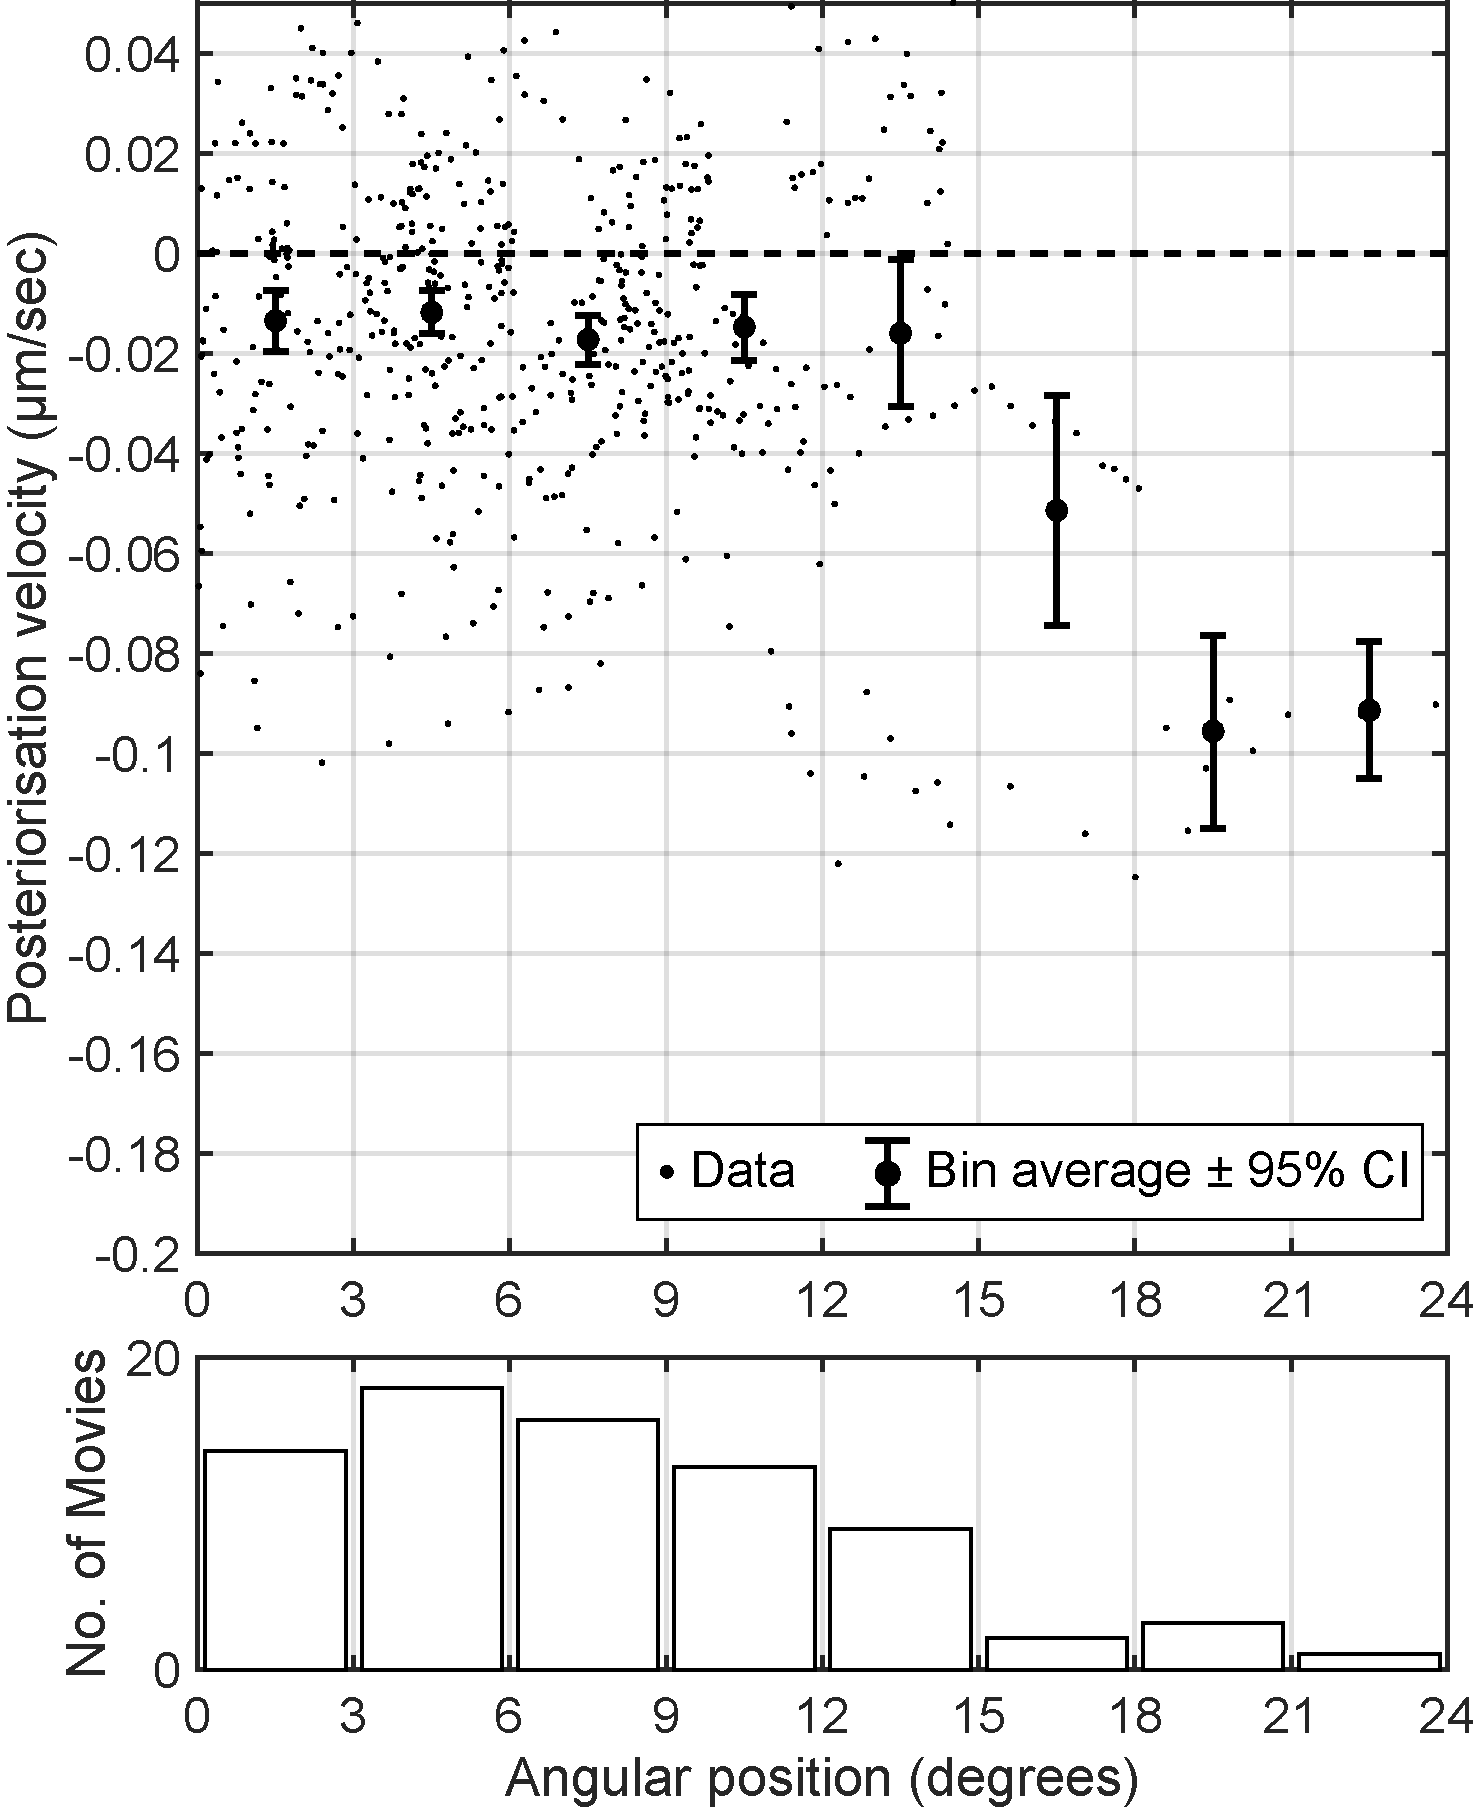
\includegraphics[width=0.95\textwidth]{Results/FigExpUnperturbed/wtPostVel.pdf}
\caption[Experimentally observed posteriorisation velocity of the male pronucleus in unperturbed embryos]{Top: Posteriorization velocity of the male pronucleus (along y-axis, in \si{\unitPostVel}) plotted against its angular position, in unperturbed embryos of SWG070 strain (N = 57). Negative values of the posteriorisation velocity indicate movement towards the posterior end. Angular position is binned using a bin width of \SI{3}{\unitAngle}. Black circles with errors bars denote the average posteriorization velocity with \num{95}\% confidence intervals in each angular position bin. Grey circles represent the data scatter -- the measured posteriorization velocities for different angular positions in each embryo (see \autoref{subsec:nucleusTracking}). Bottom: Histogram of the number of movies (along y-axis) contributing to each angular position (along x-axis) bin. A movie is considered to contribute to an angular position bin if it has any frames with angular positions within that bin. Note that a movie can contribute to multiple bins, as it may contain frames spanning different angular positions.}
\label{fig:swg070WtPostVelVsAngle}
\end{figure}

Cortical flows are also measured in unperturbed embryos using the methodology described in \autoref{sec:imageAnalysis}. Average cortical flow speed of \SI{4.12 +- 0.59}{\unitCrtxVel} is observed in unperturbed embryos. Average cortical flow fields are calculated by averaging over all embryos -- obtaining the average flow field as a function of position of the cortex and time relative to end of posteriorisation (\autoref{fig:resultsCorticalAvgFlowVsTime}). Average cortical flows fields for each angular position bin are also calculated by averaging over all frames in all embryos which have the corresponding angular position of the male pronucleus within said angular position bin (see \autoref{sec:statAnalysis} and \autoref{fig:resultsCorticalAvgFlowVsAngle}). In the latter, it is observed that the point where the cortical flows change sign correlates with the angular position -- which is expected from the role of the male pronucleus as the organiser of cortical flows during \ac{ap} axis establishment, via the centrosomes associated with the male pronucleus. These observed cortical flows are later used by the model of \ac{ap} axis alignment described in \autoref{sec:apAxisAlignmentModelMN} for calibration, to generate theoretical values of posteriorisation velocity as a function of angular positions -- see \autoref{subsec:expVsTheoryPcFurrow}.

\FloatBarrier
\section{Cortical flows are required for \acs{ap} axis alignment}\label{sec:corticalFlowsRoleMlc4}

\begin{figure}
\centering
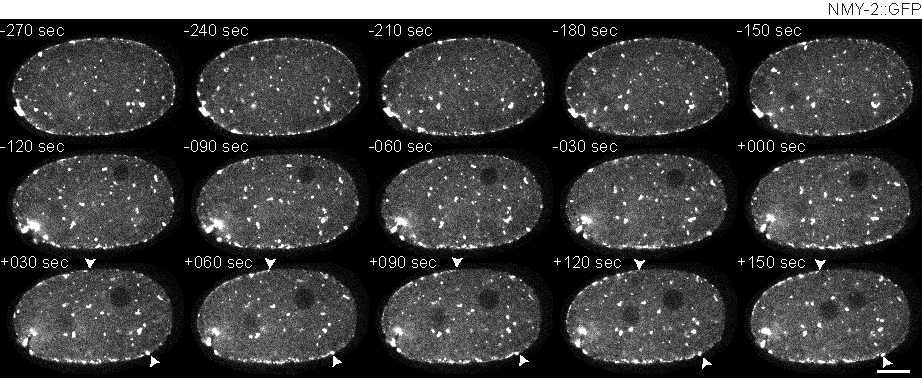
\includegraphics[width=\textwidth]{Results/FigExpMlc4/mlc4Micrograph.pdf}
\caption[Representative micrograph: \geneExp{mlc-4} \acs{rnai} embryos]{Representative \geneExp{mlc-4} \ac{rnai} embryo of SWG070 strain, labelled with \flurophoreLabel{\ac{nmy2}}{\ac{gfp}} (white), showing that male pronucleus does not posteriorise in \geneExp{mlc-4} \ac{rnai} embryos, where cortical flows are impaired. White arrows denote the depletion of myosin at the \ac{ppar} domain, which does not re-orient towards the posterior end even after t = \SI{0}{\second}. The male pronucleus can be visualized as the dark circle in the myosin channel towards the posterior end (right). t = \SI{0}{\second} is set at the end of posteriorisation of the male pronucleus -- as syncronised with the movies from unperturbed embryos of SWG070 strain. Scale bar: \SI{10}{\unitLength}. Images are rotated such that anterior and posterior ends are to the left and right respectively.}
\label{fig:swg070Mlc4Micrograph}
\end{figure}

As discussed in \autoref{sec:ApAxisEstablishment}, cortical flows play an important role in proper \ac{ap} axis establishment. A prime question to ask then is if cortical flows also play a role in \ac{ap} axis alignment. The role of cortical flows in \ac{ap} axis alignment could be understood by observing posteriorisation of the male pronucleus in embryos with impaired cortical flows. To generate embryos with reduced cortical flow velocity, \ac{rnai} of \geneExp{mlc-4} on worms of SWG070 strain was performed for a feeding time of \SI{24}{\unitRNAiTime} (see \autoref{sec:rnaiMethods} for details on \ac{rnai}). MLC-4 is a conserved regulatory light chain present in \ac{nmy2}, and is required for the \ac{nmy2} myosin motor to function \citep{shelton1999nonmuscle}. Cortical flows were found to be indeed reduced in \geneExp{mlc-4} \ac{rnai} embryos -- an average cortical flow speed of \SI{1.45 +- 0.30}{\unitCrtxVel} in \geneExp{mlc-4} \ac{rnai} embryos compared to \SI{4.12 +- 0.59}{\unitCrtxVel} in unperturbed control embryos was observed.

\begin{table}
    \centering
    \begin{tabular}{|C{0.3\textwidth}|C{0.3\textwidth}|C{0.3\textwidth}|}
        \hline
        Experimental Condition & Strain & Avg. cortical flow speed (\si{\unitCrtxVel})\\
        \hline
        Unperturbed & SWG070 & \num{4.12 +- 0.59}\\
        \geneExp{mlc-4} \ac{rnai} & SWG070 & \num{1.45 +- 0.30}\\
        \geneExp{nop-1} \ac{rnai} & SWG070 & \num{2.89 +- 0.65}\\
        \geneExp{nop-1; mel-11} \ac{rnai} & SWG070 & \num{3.34 +- 0.52}\\
        \geneExp{ima-3} \ac{rnai} & SWG070 & \num{3.99 +- 0.51}\\
        \geneExp{air-1} \ac{rnai} & SWG070 & \num{3.04 +- 0.84}\\
        \hline
        Unperturbed & SWG057 & 2.84 +- 0.37\\
        \geneExp{goa-1; gpa-16} \ac{rnai} & SWG057 & 2.62 +- 0.52\\
        \hline
    \end{tabular}
    \caption{Cortical flow speeds measured in different experimental conditions described in \autoref{ch:Results}. Average cortical flow speeds $\pm$ standard deviation are reported.}
    \label{tab:resultsCorticalFlowSpeeds}
\end{table}

\begin{figure}
\centering
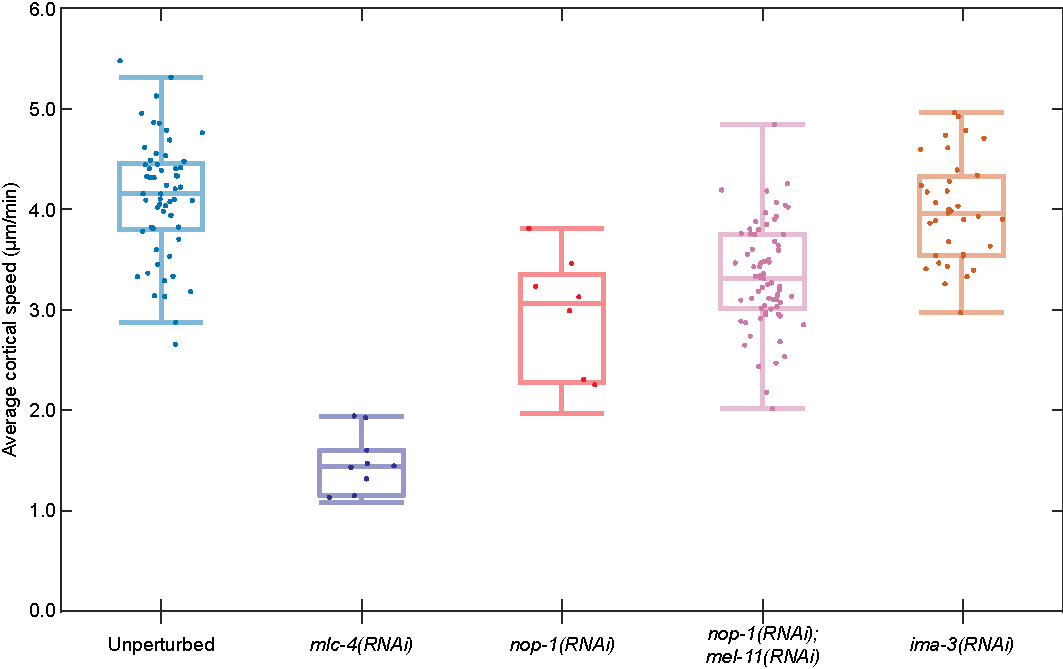
\includegraphics[width=\textwidth]{Results/FigExpCorticalFlows/crtxFlowSpeed.pdf}
\caption[Comparison of average cortical flow speed between different experimental conditions]{Average cortical flow speeds observed in different experimental conditions. Cortical flow speeds are averaged over all positions at all times for all embryos in given experimental condition. Also see \autoref{tab:resultsCorticalFlowSpeeds}}
\label{fig:resultsCorticalFlowSpeeds}
\end{figure}

\begin{figure}
\centering
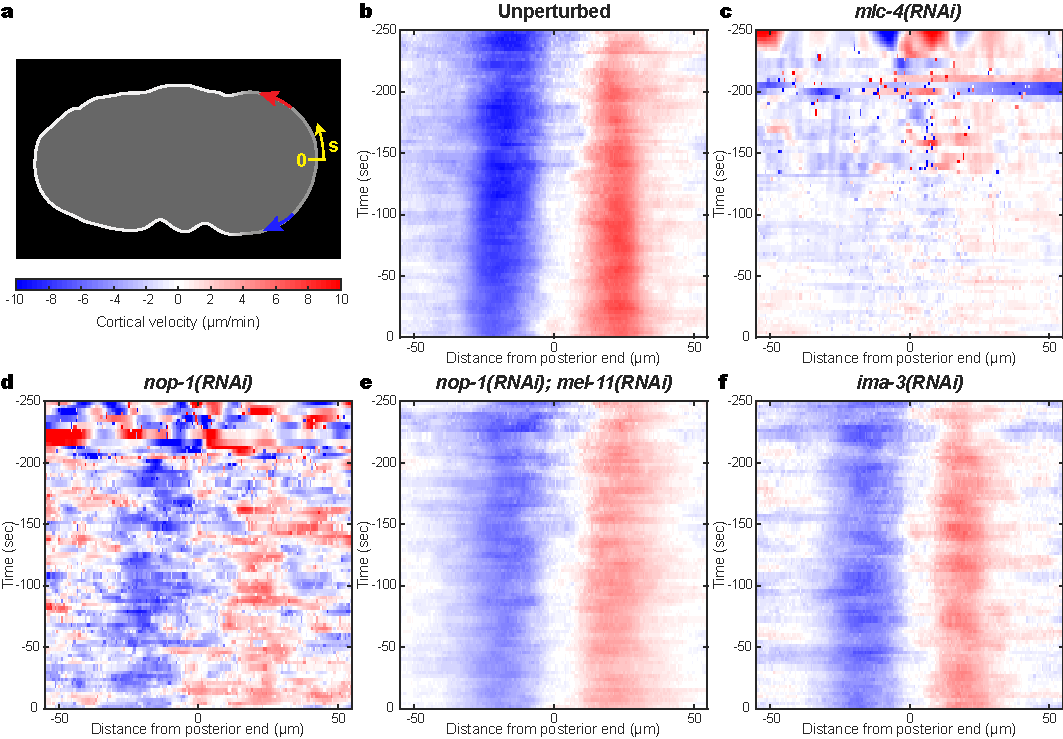
\includegraphics[width=\textwidth]{Results/FigExpCorticalFlows/crtxFlowTime.pdf}
\caption[Comparing cortical flows between different experimental conditions vs time]{Average cortical flow velocity (color, in \si{\unitCrtxVel}) plotted as a function of time (along y-axis, in \si{\second}, t = \SI{0}{\second} denotes end of posteriorization) and position on the cortex (along x-axis, in \si{\unitLength}, s=\SI{0}{\unitLength} denotes posterior end), as observed in different experimental conditions. Average cortical flow velocity at a given time and position on the cortex is obtained by averaging over cortical flows measured in all embryos at the given time and position on the cortex -- see \autoref{sec:statAnalysis}. a) Schematic. s denotes the position on the cortex, as measured along the arclength of the cortex from the posterior end (s=\SI{0}{\unitLength}). Distances in the anti-clockwise direction are considered positive. Color bar maps the colors in the plots to cortical velocity in \si{\unitCrtxVel}. Red shades indicates cortical flow pointing in the anti-clockwise direction (i.e. along the increasing direction of $s$, denoted as positive flow velocity), and blue shades in the clockwise direction (denoted as negative flow velocity). Cortical flows for (b) unperturbed embryos (N = 57), (c) \geneExp{mlc-4} RNAi embryos  (N = 10), (d) \geneExp{nop-1} RNAi embryos  (N = 9), (e) \geneExp{nop-1; mel-11} RNAi embryos  (N = 69), and (f) \geneExp{ima3} RNAi embryos (N = 35) are plotted -- all from SWG070 strain.}
\label{fig:resultsCorticalAvgFlowVsTime}
\end{figure}

\begin{figure}
\centering
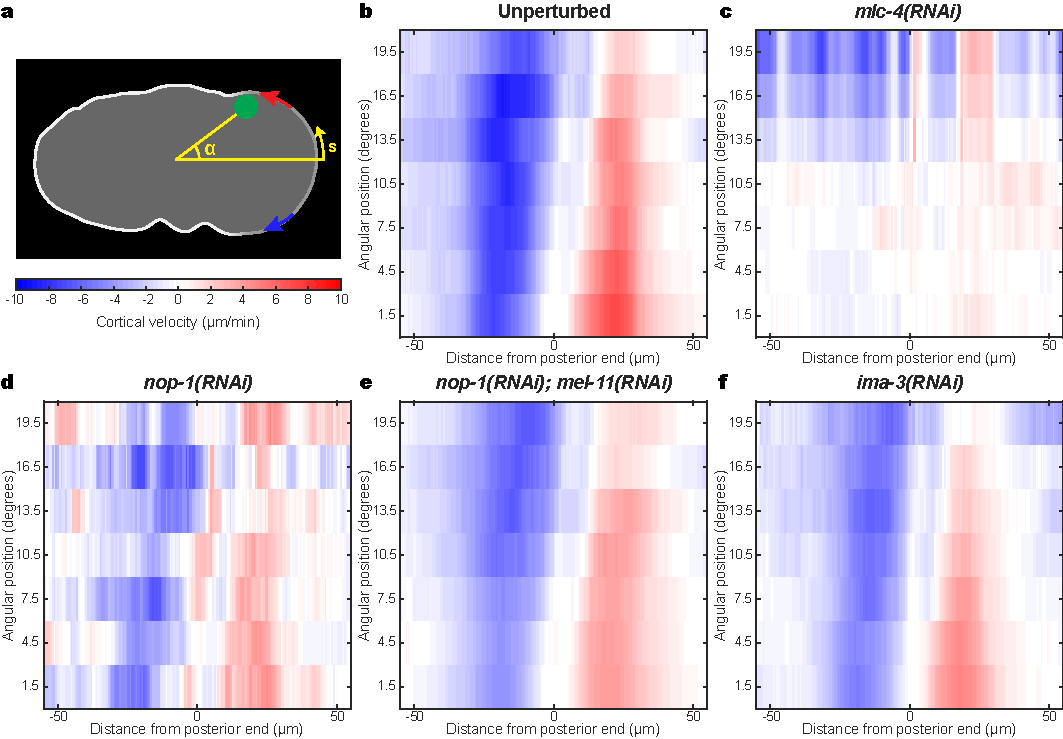
\includegraphics[width=\textwidth]{Results/FigExpCorticalFlows/crtxFlowAngle.pdf}
\caption[Comparing cortical flows between different experimental conditions vs angular positions]{Average cortical flow velocity (color, in \si{\unitCrtxVel}) plotted as a function of angular position of the male pronucleus (along y-axis, in \si{\unitAngle}) and position on the cortex (along x-axis, in \si{\unitLength}, s=\SI{0}{\unitLength} denotes posterior end), as observed in different experimental conditions. Angular positions are binned with bin width \SI{3}{\unitAngle}. Average cortical flow velocity at a given angular position bin of the male pronucleus and position on the cortex is obtained by averaging over all frames that have the corresponding angular position lie in the given angular position, at the given position on the cortex -- see \autoref{sec:statAnalysis}. a) Schematic. s denotes the position on the cortex, as measured along the arclength of the cortex from the posterior end (s=\SI{0}{\unitLength}). Distances in the anti-clockwise direction are considered positive. $\alpha$ denotes the angular position of the male pronucleus. Color bar maps the colors in the plots to cortical velocity in \si{\unitCrtxVel}. Red shades indicates cortical flow pointing in the anti-clockwise direction (i.e. along the increasing direction of $s$, denoted as positive flow velocity), and blue shades in the clockwise direction (denoted as negative flow velocity). Cortical flows for (b) unperturbed embryos (N = 57), (c) \geneExp{mlc-4} RNAi embryos  (N = 10), (d) \geneExp{nop-1} RNAi embryos  (N = 9), (e) \geneExp{nop-1; mel-11} RNAi embryos  (N = 69), and (f) \geneExp{ima3} RNAi embryos (N = 35) are plotted -- all from SWG070 strain.}
\label{fig:resultsCorticalAvgFlowVsAngle}
\end{figure}

Next, \ac{ap} axis alignment in the \geneExp{mlc-4} \ac{rnai} embryos -- in which cortical flows are impaired -- is investigated. Specifically, the posteriorisation of the male pronucleus is quantified as described before -- see \autoref{fig:swg070Mlc4Trajectories} and \autoref{fig:swg070Mlc4PostVelVsAngle}. The male pronucleus in \geneExp{mlc-4} \ac{rnai} embryos was manually tracked instead of being tracked using the image analysis pipeline described in \autoref{sec:imageAnalysis}. Posteriorisation of the male pronucleus was observed to be suppressed in these \geneExp{mlc-4} \ac{rnai} embryos: from \num{7} out of \num{10} \ac{rnai} embryos in which the male pronucleus has an initial angular position greater than \SI{5}{\unitAngle}, all were observed to fail to posteriorise -- see \autoref{fig:swg070Mlc4Trajectories}. Furthermore, almost no change is observed in angular position of the male pronucleus in \ac{rnai} embryos over time. Fitting the exponential $\alpha = \alpha_0 + \exp(-\frac{t}{t_0})$ to the plotted angular positions, as done for unperturbed embryos, results in a fit that does not converge. Instead, the best fit is found for the constant function $\alpha = \alpha_0$ with $\alpha_0 = \SI{5.45 +- 0.43}{\unitAngle}$ (see \autoref{fig:swg070Mlc4Trajectories}). Thus the migration of the male pronucleus is heavily suppressed in \geneExp{mlc-4} \ac{rnai} embryos. Such an observation is strengthened by the very slow posteriorisation velocity observed in \geneExp{mlc-4} \ac{rnai} embryos (see \autoref{fig:swg070Mlc4PostVelVsAngle} and \autoref{tab:resultsPostVelMlc4}) compared to those observed in unperturbed embryos (compare \autoref{fig:swg070WtPostVelVsAngle} and \autoref{tab:resultsPostVelUnperturbed}). Altogether, these observations lead to the conclusion that cortical flows are essential for posteriorisation of the male pronucleus, and thus \ac{ap} axis alignment.

\FloatBarrier
\begin{figure}
\centering
\begin{subfigure}[t]{0.4\textwidth}
    \centering
    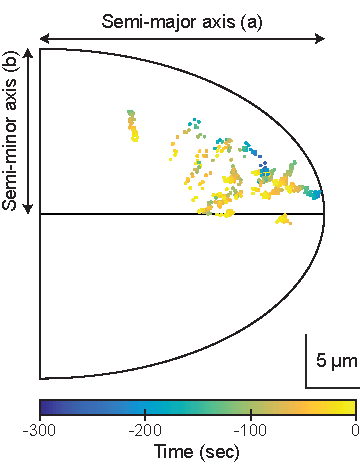
\includegraphics[width=\textwidth]{Results/FigExpMlc4/mlc4Trajectories.pdf}
    \caption{Trajectories of the male pronucleus (denoted by the coordinates of its center) observed in \geneExp{mlc-4} \ac{rnai} embryos. Color represents time. x- and y-axes lie along the long and short axes of an ellipse with semi-major axis $a = \SI{26.40}{\unitLength}$ and semi-minor axis $b = \SI{16.10}{\unitLength}$. Scale bar: \SI{5}{\unitLength}}
    \label{subfig:swg070Mlc4Trajectories-tracks}
\end{subfigure}
\hfill
\begin{subfigure}[t]{0.57\textwidth}
    \centering
    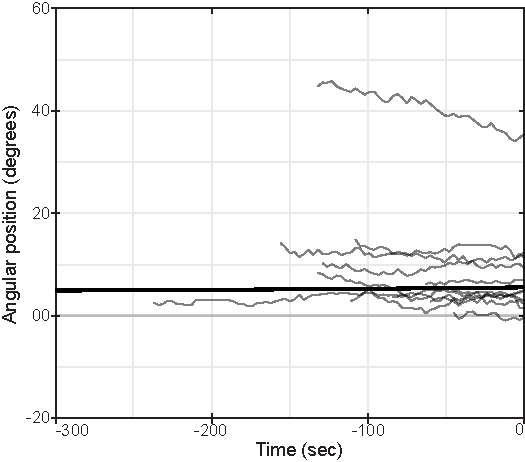
\includegraphics[width=\textwidth]{Results/FigExpMlc4/mlc4Angular.pdf}
    \caption{Angular position of the male pronucleus (on y-axis, in \si{\unitAngle}) plotted as a function of time (on x-axis, in \si{\second}), in \geneExp{mlc-4} \ac{rnai} embryos. Thin grey lines represent individual trajectories, thick black line represents a constant fit to the average of these tracks: $\alpha = \alpha_0$, with $\alpha_0 = \SI{5.45 +- 0.43}{\unitAngle}$. Note that the fit excludes the outlier trajectory around \SI{30}{\unitAngle} -- however including the trajectory in the exponential or the constant fit does not qualitatively change the result.} 
    \label{subfig:swg070Mlc4Trajectories-angleVsTime}
\end{subfigure}
\caption[Experimentally observed trajectories of the male pronucleus in \geneExp{mlc-4} \acs{rnai} embryos]{Experimentally observed trajectories of the male pronucleus during posteriorisation in \geneExp{mlc-4} \ac{rnai} embryos of SWG070 strain (N = 10). Male pronucleus is manually tracked in \geneExp{mlc-4} \ac{rnai} embryos. Average semi-major and semi-minor axes lengths for \geneExp{mlc-4} \ac{rnai} embryos of SWG070 strain are used in \autoref{subfig:swg070Mlc4Trajectories-tracks} -- see \autoref{tab:resultsEmbryoGeometry}. Angular position is defined as the angle between the long axis and line connecting the centers of the male pronucleus and embryo. t = \SI{0}{\second} denotes end of posteriorisation.}
\label{fig:swg070Mlc4Trajectories}
\end{figure}

\begin{table}
    \centering
    \begin{tabular}{|C{0.2\textwidth}|C{0.45\textwidth}|C{0.2\textwidth}|}
        \hline
        Angular positions (\si{\unitAngle}) & Posteriorisation velocity (\SI{1e-1}{\unitPostVel}) & No. of embryos\\
        \hline
        \numrange{0}{3} & \num{-0.03} (\num{-0.08},\num{0.01}) & 4\\
        \numrange{3}{6} & \num{-0.02} (\num{-0.01},\num{0.05}) & 5\\
        \numrange{6}{9} & \num{-0.02} (\num{-0.07},\num{0.03}) & 3\\
        \numrange{9}{12} & \num{-0.02} (\num{-0.07},\num{0.02}) & 2\\
        \numrange{12}{15} & \num{-0.3} (\num{-0.4},\num{-0.17}) & 1\\
        \hline
    \end{tabular}
    \caption{Posteriorisation velocity measured for each angular position bin in \geneExp{mlc-4} \ac{rnai} embryos. Average posteriorisation velocity along with \num{95}\% confidence interval for the average are reported.}
    \label{tab:resultsPostVelMlc4}
\end{table}

\begin{figure}[p]
\centering
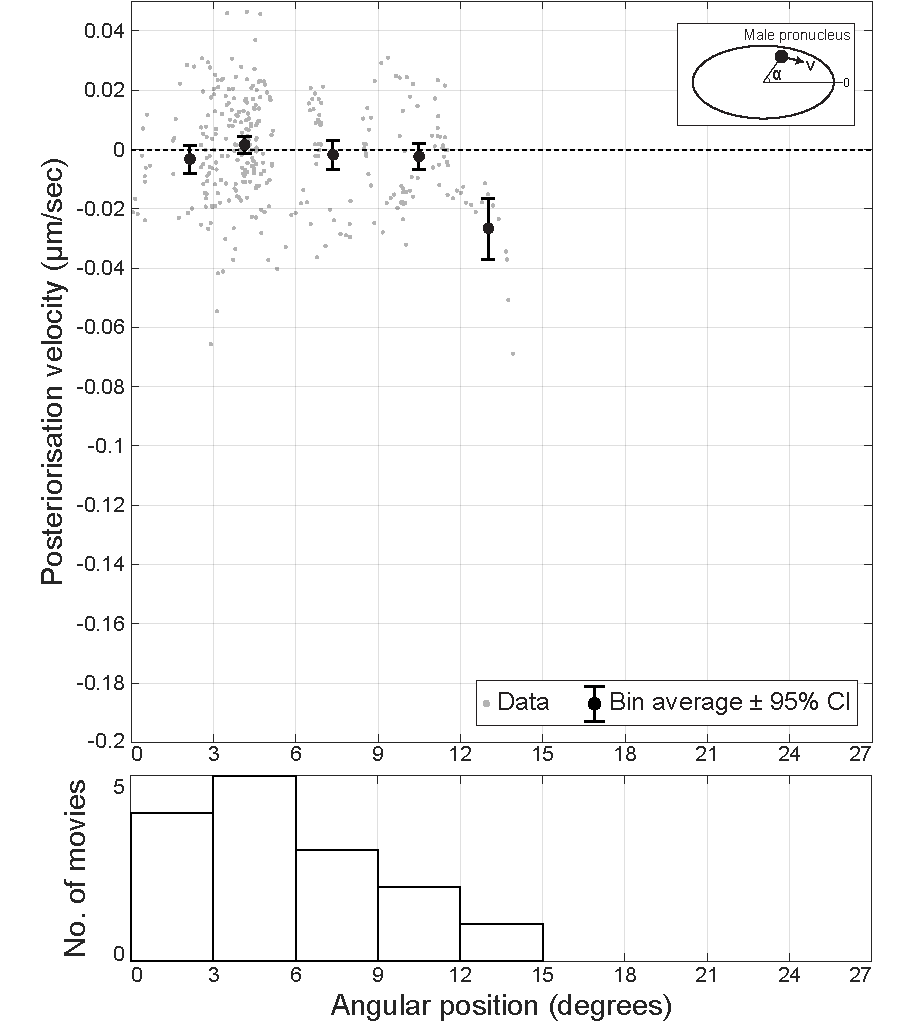
\includegraphics[width=0.95\textwidth]{Results/FigExpMlc4/mlc4PostVel.pdf}
\caption[Experimentally observed posteriorisation velocity of the male pronucleus in \geneExp{mlc-4} \acs{rnai} embryos]{Top: Posteriorization velocity of the male pronucleus (along y-axis, in \si{\unitPostVel}) plotted against its angular position, in \geneExp{mlc-4} \ac{rnai} embryos of SWG070 strain (N = 10). Negative values of the posteriorisation velocity indicate movement towards the posterior end. Angular position is binned with bin width of \SI{3}{\unitAngle}. Black circles with errors bars denote average posteriorization velocity with \num{95}\% confidence intervals in each angular position bin. Grey circles represent data scatter -- measured posteriorization velocities for different angular positions in each embryo (calculated as described in \autoref{subsec:nucleusTracking} after manual tracking). Bottom: Histogram of the number of movies (along y-axis) contributing to each angular position (along x-axis) bin. A movie contributes to an angular position bin if it has any frames with angular positions within that bin. Note that a movie can contribute to multiple bins, as it may contain frames spanning different angular positions. Data was only available until \SI{15}{\unitAngle}}
\label{fig:swg070Mlc4PostVelVsAngle}
\end{figure}

\FloatBarrier
\section{Role of Pseudocleavage furrow in \acs{ap} axis alignment}\label{sec:PcFurrowRole}
As discussed in \autoref{subsec:ApAxisAlignment}, cortical flows during \ac{ap} axis establishment can lead to two consequences -- flows within the bulk cytoplasm \citep{niwayama2011hydrodynamic} and formation of the pseudocleavage furrow \citep{reymann2016cortical}. Two different mechanisms of \ac{ap} axis alignment -- cytoplasmic flow-dependent mechanism and pseudocleavage furrow-dependent mechanism -- that arise from each of the two consequence were discussed in \autoref{subsec:ApAxisAlignment}. In this section, the contributions of these two mechanisms is evaluated using experiments that remove the pseudocleavage furrow and corresponding numerical simulations of the theoretical model described in \autoref{sec:apAxisAlignmentModelMN}.

\subsection{Removing Pseudocleavage furrow via \acs{rnai}}\label{subsec:Nop1AndNop1Mel11}

\begin{figure}
\centering
\begin{subfigure}{\textwidth}
    \centering
    \includegraphics[width=\textwidth]{Results/FigExpNop1Mel11/nop1Micrograph.pdf}
    \caption{Representative \geneExp{nop-1} \ac{rnai} embryo of SWG070 strain, labelled with \flurophoreLabel{\ac{nmy2}}{\ac{gfp}} (white), showing the lack of pseudocleavage furrow in \geneExp{nop-1} \ac{rnai} embryos.}
    \label{subfig:swg070Nop1AndNop1Mel11Micrograph-nop1}
\end{subfigure}
\hfill
\begin{subfigure}{\textwidth}
    \centering
    \includegraphics[width=\textwidth]{Results/FigExpNop1Mel11/nop1mel11Micrograph.pdf}
    \caption{Representative \geneExp{nop-1; mel-11} double \ac{rnai} embryo of SWG070 strain, labelled with \flurophoreLabel{\ac{nmy2}}{\ac{gfp}} (white), showing the lack of pseudocleavage furrow in \geneExp{nop-1; mel-11} \ac{rnai} embryos.}
    \label{subfig:swg070Nop1AndNop1Mel11Micrograph-nop1mel11}
\end{subfigure}
\caption[Representative micrograph: \geneExp{nop-1} \acs{rnai} and \geneExp{nop-1; mel-11} double \acs{rnai} embryos]{Representative \geneExp{nop-1} \ac{rnai} embryo and \geneExp{nop-1; mel-11} double \ac{rnai} embryo of SWG070 strain, labelled with \flurophoreLabel{\ac{nmy2}}{\ac{gfp}} (white), showing the lack of pseudocleavage furrow in both \geneExp{nop-1} \ac{rnai} and \geneExp{nop-1; mel-11} \ac{rnai} embryos. Compare to representative unperturbed embryo depicted in \autoref{fig:swg070WtMicrograph} and pseudocleavage furrow depicted in \autoref{fig:apAxisAlignment}. The male pronucleus can be visualized as the dark circle in the myosin channel towards the posterior end. t = \SI{0}{\second} is set at the end of posteriorisation of the male pronucleus. Scale bar: \SI{10}{\unitLength} in each. Images are rotated such that anterior and posterior ends are to the left and right respectively.}
\label{fig:swg070Nop1AndNop1Mel11Micrograph}
\end{figure}

To understand the role of the pseudocleavage furrow-dependent mechanism in \ac{ap} axis alignment, posteriorisation of the male pronucleus was quantified in embryos lacking a pseudocleavage furrow. Such embryos were generated via \ac{rnai} of \geneExp{nop-1} on worms of SWG070 strain for a feeding time of \SI{24}{\unitRNAiTime} (see \autoref{sec:rnaiMethods} for details on \ac{rnai}). NOP-1 modulates activity of the small GTPase RHO-1, which is a major regulator of the activity of the actomyosin cortex in the \ac{ce} embryo \citep{tse2012nop1}. Embryos generated by worms which are mutant for NOP-1 (that is, possess a non-functional form of NOP-1) have been observed to lack a pseudocleavage furrow \citep{rose1995pseudocleavage}. While it was observed that \geneExp{nop-1} \ac{rnai} embryos do indeed lack a pseudocleavage furrow (\num{8} out of \num{9} embryos), these embryos also showed reduced cortical flow speeds, with average cortical flow speed of \SI{2.89 +- 0.65}{\unitCrtxVel} in \geneExp{nop-1} \ac{rnai} embryos compared to \SI{4.12 +- 0.59}{\unitCrtxVel} observed in unperturbed embryos (see \autoref{tab:resultsCorticalFlowSpeeds}, \autoref{fig:resultsCorticalFlowSpeeds}, \autoref{fig:resultsCorticalAvgFlowVsTime} and \autoref{fig:resultsCorticalAvgFlowVsAngle}).

To generate pseudocleavage furrow-deficient embryos with cortical flows comparable to those observed in unperturbed embryos (which do possess a pseudocleavage furrow), a double \ac{rnai} of \geneExp{nop-1} and \geneExp{mel-11} was performed on worms of SWG070 strain for a feeding time of \SI{24}{\unitRNAiTime} (see \autoref{sec:rnaiMethods} for details on double \ac{rnai}). MEL-11 is a myosin phosphatase \citep{piekny2002rho} that suppresses the activity of myosin in the cortex \citep{najafabadi2022orchestrating}. The \geneExp{nop-1; mel-11} \ac{rnai} embryos thus generated lack a pseudocleavage furrow (\num{69} out of \num{69} embryos). Furthermore, experimental measurement of cortical flows in \geneExp{nop-1; mel-11} \ac{rnai} embryos yields average cortical flow speed of \SI{3.34 +- 0.52}{\unitCrtxVel} in \geneExp{nop-1; mel-11} \ac{rnai} embryos, comparable to the average cortical flow speed \SI{4.12 +- 0.59}{\unitCrtxVel} observed in unperturbed embryos (see \autoref{tab:resultsCorticalFlowSpeeds}, \autoref{fig:resultsCorticalFlowSpeeds}, \autoref{fig:resultsCorticalAvgFlowVsTime} and \autoref{fig:resultsCorticalAvgFlowVsAngle}). Thus, the double \ac{rnai} of \geneExp{nop-1} and \geneExp{mel-11} leads to the required pseudocleavage furrow-deficient embryos with cortical flows comparable to those observed in unperturbed embryos.

Next, the \ac{ap} axis alignment process in these \geneExp{nop-1; mel-11} \ac{rnai} embryos -- which lack a pseudocleavage furrow -- is investigated. Specifically, the posteriorisation of the male pronucleus is quantified as described before -- see \autoref{fig:swg070Nop1Mel11Trajectories} and \autoref{fig:swg070Nop1Mel11PostVelVsAngle}, using the image analysis pipeline described in \autoref{sec:imageAnalysis}. Angular positions in the pseudocleavage furrow-deficient embryos were generally observed to decrease towards \SI{0}{\unitAngle} as time reaches closer to end of posteriorisation (t = \SI{0}{\second}), albeit at a slower rate compared to that observed for unperturbed embryos (\autoref{fig:swg070Nop1Mel11Trajectories}). Specifically, this decay towards \SI{0}{\unitAngle} was quantified by fitting an exponential $\alpha = \alpha_0 + \exp(-\frac{t}{t_0})$ to the plotted angular positions, yielding a time constant $t_0 = \SI{201 +- 24}{\second}$ and $\alpha_0 = \SI{-0.75 +- 0.3}{\unitAngle}$ (\autoref{fig:swg070Nop1Mel11Trajectories}). Note that the time constant $t_0 = \SI{201 +- 24}{\second}$ for the pseudocleavage furrow-deficient embryos is larger than that found for the unperturbed embryos $t_0 = \SI{119 +- 3}{\second}$ -- indicating a slower posteriorisation of the male pronucleus in the pseudocleavage furrow-deficient embryos compared to that observed in unperturbed embryos. 

\begin{figure}
\centering
\begin{subfigure}[t]{0.4\textwidth}
    \centering
    \includegraphics[width=\textwidth]{Results/FigExpNop1Mel11/nop1mel11Trajectories.pdf}
    \caption{Trajectories of the male pronucleus (denoted by the coordinates of its center) observed in \geneExp{nop-1; mel-11} \ac{rnai} embryos. Color represents time. x- and y-axes lie along the long and short axes of an ellipse with semi-major axis $a = \SI{26.4}{\unitLength}$ and semi-minor axis $b = \SI{16.1}{\unitLength}$. Scale bar: \SI{5}{\unitLength}}
    \label{subfig:swg070Nop1Mel11Trajectories-tracks}
\end{subfigure}
\hfill
\begin{subfigure}[t]{0.57\textwidth}
    \centering
    \includegraphics[width=\textwidth]{Results/FigExpNop1Mel11/nop1mel11Angular.pdf}
    \caption{Angular position of the male pronucleus (on y-axis, in \si{\unitAngle}) plotted as a function of time (on x-axis, in \si{\second}), in \geneExp{nop-1; mel-11} \ac{rnai} embryos. Thin grey lines represent individual trajectories, thick black line represents a exponential fit to the average of these tracks: $\alpha = \alpha_0 + \exp(-\frac{t}{t_0})$, with $t_0 = \SI{201 +- 24}{\second}$ and $\alpha_0 = \SI{-0.75 +- 0.3}{\unitAngle}$.} 
    \label{subfig:swg070Nop1Mel11Trajectories-angleVsTime}
\end{subfigure}
\caption[Experimentally observed trajectories of the male pronucleus in \geneExp{nop-1; mel-11} embryos]{Experimentally observed trajectories of the male pronucleus during posteriorisation in \geneExp{nop-1; mel-11} embryos of SWG070 strain (N = 69). See \autoref{subsec:nucleusTracking} for details on male pronucleus tracking. Average semi-major and semi-minor axes lengths for \geneExp{nop-1; mel-11} embryos of SWG070 strain are used in \autoref{subfig:swg070Nop1Mel11Trajectories-tracks} -- see \autoref{tab:resultsEmbryoGeometry}. Angular position is defined as the angle between the long axis and line connecting the centers of the male pronucleus and embryo. t = \SI{0}{\second} denotes end of posteriorisation.}
\label{fig:swg070Nop1Mel11Trajectories}
\end{figure}

Posteriorisation velocity of the male pronucleus in the pseudocleavage furrow-deficient embryos, plotted as a function of angular position (see \autoref{sec:statAnalysis} for details on binning of angular positions), demonstrate that the male pronucleus is, on average, moving towards the posterior end (as indicated by the negative sign of the velocity) -- with higher speed at higher angular positions (\autoref{fig:swg070Nop1Mel11PostVelVsAngle}, \autoref{tab:resultsPostVelNop1Mel11}). This is qualitatively similar to the observations made for the unperturbed embryos (\autoref{fig:swg070WtPostVelVsAngle}, \autoref{tab:resultsPostVelUnperturbed}). However, on comparison with the posteriorisation velocity observed in the latter, it is observed that the posteriorisation velocity of the male pronucleus observed in the pseudocleavage furrow-deficient embryos are consistently slower that those observed in the unperturbed embryos, with larger difference between the two at higher angular positions. 

\begin{table}
    \centering
    \begin{tabular}{|C{0.2\textwidth}|C{0.55\textwidth}|C{0.2\textwidth}|}
        \hline
        Angular positions (\si{\unitAngle}) & Posteriorisation velocity (\SI{1e-1}{\unitPostVel}) & No. of embryos\\
        \hline
        \numrange{0}{3} & \num{-0.10} (\num{-0.12},\num{-0.08}) & 37\\
        \numrange{3}{6} & \num{-0.14} (\num{-0.17},\num{-0.11}) & 36\\
        \numrange{6}{9} & \num{-0.14} (\num{-0.17},\num{-0.11}) & 29\\
        \numrange{9}{12} & \num{-0.17} (\num{-0.21},\num{-0.13}) & 19\\
        \numrange{12}{15} & \num{-0.17} (\num{-0.21},\num{-0.13}) & 19\\
        \numrange{15}{18} & \num{-0.20} (\num{-0.25},\num{-0.16}) & 13\\
        \numrange{18}{21} & \num{-0.20} (\num{-0.25},\num{-0.16}) & 12\\
        \numrange{21}{24} & \num{-0.36} (\num{-0.44},\num{-0.29}) & 8\\
        \numrange{24}{27} & \num{-0.10} (\num{-0.15},\num{-0.05}) & 3\\
        \hline
    \end{tabular}
    \caption{Posteriorisation velocity measured for each angular position bin in \geneExp{nop-1; mel-11} \ac{rnai} embryos. Average posteriorisation velocity along with \num{95}\% confidence interval for the average are reported.}
    \label{tab:resultsPostVelNop1Mel11}
\end{table}

\begin{figure}[p]
\centering
\includegraphics[width=0.95\textwidth]{Results/FigExpNop1Mel11/nop1mel11PostVel.pdf}
\caption[Experimentally observed posteriorisation velocity of the male pronucleus in \geneExp{nop-1; mel-11} \acs{rnai} embryos]{Top: Posteriorization velocity of the male pronucleus (along y-axis, in \si{\unitPostVel}) plotted against its angular position, in \geneExp{nop-1; mel-11} \ac{rnai} embryos of SWG070 strain (N = 69). Negative values of the posteriorisation velocity indicate movement towards the posterior end. Angular position is binned using a bin width of \SI{3}{\unitAngle}. Black circles with errors bars denote the average posteriorization velocity with \num{95}\% confidence intervals in each angular position bin. Grey circles represent the data scatter -- the measured posteriorization velocities for different angular positions in each embryo (see \autoref{subsec:nucleusTracking}). Bottom: Histogram of the number of movies (along y-axis) contributing to each angular position (along x-axis) bin. A movie is considered to contribute to an angular position bin if it has any frames with angular positions within that bin. Note that a movie can contribute to multiple bins, as it may contain frames spanning different angular positions.}
\label{fig:swg070Nop1Mel11PostVelVsAngle}
\end{figure}

Altogether, these experimental observations indicate that the rate of \ac{ap} axis alignment is diminished in the absence of the pseudocleavage furrow. In other words, experimental removal of pseudocleavage furrow via a double \geneExp{nop-1; mel-11} \ac{rnai} indicates that the pseudocleavage furrow is important for the dynamics of \ac{ap} axis alignment, and to ensure the alignment of the \ac{ap} axis at the rate observed in the unperturbed embryos. However, the pseudocleavage furrow is not essential for \ac{ap} axis alignment -- embryos deficient in the pseudocleavage furrow can still exhibit \ac{ap} axis alignment, albeit at a slower rate.

\FloatBarrier
\subsection{Comparing numerical simulations to experimental results}\label{subsec:expVsTheoryPcFurrow}
\subsubsection{Theoretical model accounts for \acs{ap} axis alignment in unperturbed controls}\label{subsubsec:fullModelForWT}
To further probe the role of the pseudocleavage furrow in \ac{ap} axis alignment, these experimental observations are compared to numerical simulations of the theoretical model of \ac{ap} axis alignment. As described in \autoref{sec:apAxisAlignmentModelMN} and \autoref{subsec:ApAxisAlignment}, the theoretical model considers two possible mechanisms of \ac{ap} axis alignment: cytoplasmic flow-dependent mechanism, and pseudocleavage furrow-dependent mechanism. Comparisons of experimental observations in unperturbed embryos -- which possess a pseudocleavage furrow -- and \geneExp{nop-1; mel-11} \ac{rnai} embryos -- which lack a pseudocleavage furrow with numerical simulations of the theoretical model could then yield insights into the contributions of the two mechanisms to \ac{ap} axis alignment.

First, the theoretical model is compared with observations in the unperturbed embryo. Specifically, posteriorisation velocity of the male pronucleus as a function of its angular position, and the trajectory of the male pronucleus (that is, angular position as a function of time) are calculated (see \autoref{sec:apAxisAlignmentModelMN} for details) using the full theoretical model -- that is, including the pseudocleavage furrow-dependent mechanism, as unperturbed embryos possess a pseudocleavage furrow. Quantities calculated from the the theoretical model are then compared to those observed in the experiments with unperturbed embryos. 

Numerical simulations of the theoretical model requires calibration of model parameters using the experimentally measured cortical flows. Note that the model is evaluated (in this section) on an ellipsoid with the same axes lengths as the average axes lengths for the unperturbed embryos: \longAxisLength = \SI{28.9}{\unitLength} (semi-major axis), \shortAxisLength = \SI{16.4}{\unitLength} -- see \autoref{tab:resultsEmbryoGeometry}. In brief, the calibration procedure varies the following model parameters: hydrodynamic length \hydrodynamicLength, active force relaxation \activeRelaxLength and nematic stress relaxation \nematicLength. Cortical flows calculated using the varied parameters are then compared to those experimentally measured. This is done for a range of angular positions of the male pronucleus, using the average cortical flows observed for angular position bin (with bin width of \SI{3}{\unitAngle}, shown in \autoref{fig:resultsCorticalAvgFlowVsAngle} -- see \autoref{sec:statAnalysis} for details on methodology). Angular positions upto \SI{21}{\unitAngle} only are considered for the calibration procedure, due to worse quality of data for higher angular positions as the number of movies contributing to those angular position bins decreases. The calibration procedure results in values of \hydrodynamicLength, \activeRelaxLength and \nematicLength that ensure best match with experimentally measured cortical flows. A detailed discussion on the calibration process can be found in \autoref{subsec:numericsModelMN}. 

\begin{figure}
    \centering
    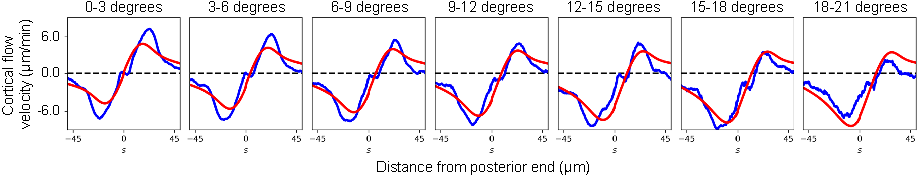
\includegraphics[width=\textwidth]{Results/FigComparePCF/wtCorticalFlowModel.pdf}
    \caption[Calibrating theoretical model using cortical flows observed in unperturbed embryos]{Comparison of observed cortical flows in unperturbed embryos of SWG070 strain to those calculated by the theoretical model of \ac{ap} axis alignment. Blue line denotes the average cortical flow velocity observed in unperturbed embryos, plotted as a function of position along the cortex $s$ in each angular position bin -- also depicted in \autoref{fig:resultsCorticalAvgFlowVsAngle}. Red denotes the cortical flow velocity calculated by the theoretical model after calibration, with model parameters: \hydrodynamicLength = \SI{10}{\unitLength}, \activeRelaxLength = \SI{11.5}{\square\unitLength\per\second}, \nematicLength = \SI{152.5}{\square\unitLength\per\second}.}
    \label{fig:unperturbedModelCalibrationCorticalFlows}
\end{figure}

For the experimentally measured cortical flows in unperturbed embryos, the calibration procedure yields the following model parameters: \hydrodynamicLength = \SI{10}{\unitLength}, \activeRelaxLength = \SI{11.5}{\square\unitLength\per\second}, \nematicLength = \SI{152.5}{\square\unitLength\per\second} -- see \autoref{fig:unperturbedModelCalibrationCorticalFlows}. In the theoretical model, bulk cytoplasmic flows are determined uniquely from the calculated cortical flows via the no-slip boundary condition (see \autoref{subsec:cytoplasmPronucleusModelMN}). Comparison of experimentally measured cortical and cytoplasmic flows (see \autoref{subsec:corticalFlows} and \autoref{subsec:cytoFlows} for methodology) with calculated cortical and cytoplasmic flows shows a good agreement between the two -- see \autoref{fig:unperturbedModelCalibrationCorticalFlows} and \autoref{fig:unperturbedModelCalibrationCorticalAndCytoFlows}. Thus, the theoretical model can faithfully recapitulate the experimental cortical and cytoplasmic flows, for the selected set of model parameters.

\begin{figure}
    \centering
    \includegraphics{Results/FigComparePCF/cytoFlowCompare.pdf}
    \caption[Flows observed in unperturbed embryos compared to those calculated by theoretical model]{Comparison of observed cortical and cytoplasmic flows in unperturbed embryos of SWG070 strain (left) to those calculated by the theoretical model of \ac{ap} axis alignment (right) with model parameters: \hydrodynamicLength = \SI{10}{\unitLength}, \activeRelaxLength = \SI{11.5}{\square\unitLength\per\second}, \nematicLength = \SI{152.5}{\square\unitLength\per\second} (referred to as the unperturbed model), for three angular positions (\SI{0}{\unitAngle}, \SI{5}{\unitAngle}, \SI{10}{\unitAngle}) of the male pronucleus (black shaded circle).In each panel, ellipse interior represents cytoplasmic flows, and outer ellipse represents cortical flows. See colorbar for magnitude of flow velocities.}
    \label{fig:unperturbedModelCalibrationCorticalAndCytoFlows}
\end{figure}

Comparison of the experimentally observed posteriorisation velocity of the male pronucleus with those calculated using the model fix the final model parameter \dragCoefficient. This parameter captures the direct interactions between the male pronucleus and the cortex (see \autoref{subsec:cytoplasmPronucleusModelMN}). For the set of model parameters obtained via calibration for the unperturbed embryos, \dragCoefficient = \num{0.61} to ensure that the calculated posteriorisation velocity best match the observed posteriorization velocity as a function of angular position of the male pronucleus -- see \autoref{subfig:unperturbedModelCompareExpt-postVel} and \autoref{tab:resultsPostVelUnperturbedVsFullModel}. With these model parameters, the calculated posteriorisation velocity agrees with experimentally observed average posteriorisation velocity in unperturbed embryos, for angular positions upto \SI{21}{\unitAngle}. For higher angular positions, average posteriorisation velocity observed in experiments is faster compared to calculated posteriorisation velocity for the same angular position. By integrating the calculated posteriorisation velocity (as a function of angular position), the calculated trajectory of the male pronucleus -- referring to the calculated angular position of the male pronucleus as a function of time relative to end of posteriorisation -- can also be obtained (see \autoref{subsec:numericsModelMN}), which is observed to agree well with the experimentally observed trajectories of the male pronucleus -- see \autoref{subfig:unperturbedModelCompareExpt-tracks}.

\begin{table}
    \centering
    \begin{tabular}{|C{0.2\textwidth}|C{0.35\textwidth}|C{0.35\textwidth}|}
        \hline
        Angular positions (\si{\unitAngle}) & Experimental post. velocity (\SI{1e-1}{\unitPostVel}) & Calculated post. velocity (\SI{1e-1}{\unitPostVel})\\
        \hline
        \numrange{0}{3} & \num{-0.15} (\num{-0.18},\num{-0.13}) & \num{-0.09}\\
        \numrange{3}{6} & \num{-0.17} (\num{-0.20},\num{-0.14}) & \num{-0.22}\\
        \numrange{6}{9} & \num{-0.27} (\num{-0.30},\num{-0.23}) & \num{-0.30}\\
        \numrange{9}{12} & \num{-0.40} (\num{-0.46},\num{-0.35}) & \num{-0.38}\\
        \numrange{12}{15} & \num{-0.46} (\num{-0.52},\num{-0.41}) & \num{-0.45}\\
        \numrange{15}{18} & \num{-0.40} (\num{-0.47},\num{-0.34}) & \num{-0.47}\\
        \numrange{18}{21} & \num{-0.49} (\num{-0.58},\num{-0.40}) & \num{-0.48}\\
        \numrange{21}{24} & \num{-0.85} (\num{-0.98},\num{-0.72}) & \num{-0.47}\\
        \hline
    \end{tabular}
    \caption{Experimentally observed posteriorisation velocity for each angular position bin in unperturbed embryos compared with those calculated by the unperturbed model (theoretical model evaluated with model parameters: \hydrodynamicLength = \SI{10}{\unitLength}, \activeRelaxLength = \SI{11.5}{\square\unitLength\per\second}, \nematicLength = \SI{152.5}{\square\unitLength\per\second}, \dragCoefficient = \num{0.61}). Experimental Post. velocity: Average posteriorisation velocity along with \num{95}\% confidence interval for each angular position bin observed in unperturbed embryos (see \autoref{tab:resultsPostVelUnperturbed} and \autoref{fig:swg070WtPostVelVsAngle}. Calculated Post. velocity: Posteriorisation velocity calculated at center of angular position bin by theoretical model with model parameters: \hydrodynamicLength = \SI{10}{\unitLength}, \activeRelaxLength = \SI{11.5}{\square\unitLength\per\second}, \nematicLength = \SI{152.5}{\square\unitLength\per\second}, \dragCoefficient = \num{0.61}.}
    \label{tab:resultsPostVelUnperturbedVsFullModel}
\end{table}

\begin{figure}
    \centering
    \begin{subfigure}[t]{0.45\textwidth}
        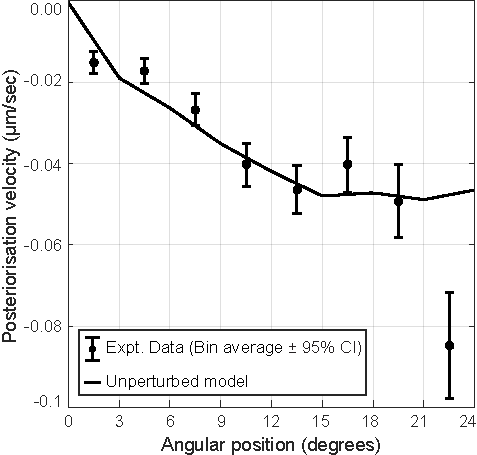
\includegraphics[width=\textwidth]{Results/FigComparePCF/wtPostVelModel.pdf}
        \caption{Comparing average posteriorisation velocity of the male pronucleus (black circles with error bars, \num{95}\% confidence interval) in unperturbed embryos (from \autoref{fig:swg070WtPostVelVsAngle}) with that calculated by unperturbed model (black line), both plotted against angular position of the male pronucleus. Posteriorisation velocity is on y-axis (in \si{\unitPostVel}, negative velocity indicate movement towards posterior end), and angular position on x-axis (in \si{\unitAngle}).}
        \label{subfig:unperturbedModelCompareExpt-postVel}
    \end{subfigure}
    \hfill
    \begin{subfigure}[t]{0.45\textwidth}
        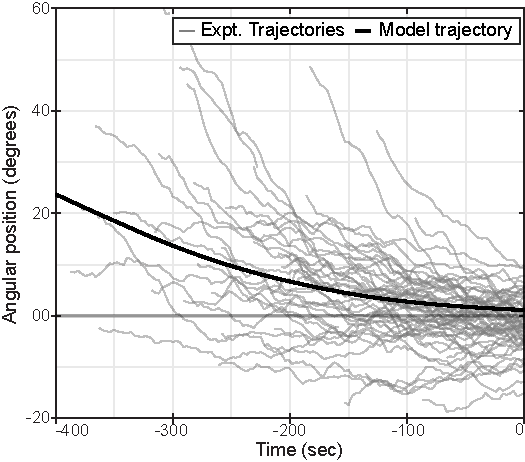
\includegraphics[width=\textwidth]{Results/FigComparePCF/wtTrajectoriesModel.pdf}
        \caption{Comparing angular positions of the male pronucleus (y-axis, in \si{\unitAngle}) observed in unperturbed embryos (thin grey lines, from \autoref{fig:swg070WtTrajectories}) with the calculated trajectory of the male pronucleus (thick black line) from unperturbed model, both plotted against time (on x-axis, in \si{\second}, t = \SI{0}{\second} denotes end of posteriorisation).}
        \label{subfig:unperturbedModelCompareExpt-tracks}
    \end{subfigure}
    \caption[Experimentally observed posteriorisation in unperturbed embryos compared with that calculated by theoretical model]{Comparing experimentally observed posteriorisation of the male pronucleus in unperturbed embryos of the SWG070 strain with that calculated by the unperturbed model. Unperturbed model refers to the theoretical model of \ac{ap} axis alignment evaluated with the following model parameters: \hydrodynamicLength = \SI{10}{\unitLength}, \activeRelaxLength = \SI{11.5}{\square\unitLength\per\second}, \nematicLength = \SI{152.5}{\square\unitLength\per\second}, \dragCoefficient = \num{0.61}. \dragCoefficient = \num{0.61} is selected to best match the average posteriorisation velocity observed in unperturbed embryos of the SWG070 strain, depicted in \autoref{subfig:unperturbedModelCompareExpt-postVel}.}
    \label{fig:unperturbedModelCompareExpt}
\end{figure} 

The sensitivity of the calculated posteriorisation velocity to the calibrated model parameters was also investigated. Specifically, \hydrodynamicLength and \nematicLength were separately varied to $\pm\num{50}\%$ of their calibrated values -- see \autoref{fig:unperturbedModelParameterVary}, \autoref{tab:resultsPostVelFullModelVaryLh} and \autoref{tab:resultsPostVelFullModelVaryLn}. As discussed in \autoref{subsec:numericsModelMN}, \activeRelaxLength scales with the cortical flow velocity, and therefore is set separately. Posteriorisation velocity of the male pronucleus is then calculated using the varied model parameters and then compared again to those experimentally measured in unperturbed embryos. It is observed that the calculated posteriorisation velocity still retain similar qualitative features as those experimentally measured in unperturbed embryos: Posteriorisation velocity calculated after model parameter variation remain comparable to the average posteriorisation velocity observed in experiments for angular positions upto \SI{21}{\unitAngle}. Thus, the calculated posteriorisation velocity is robust to variations in the calibration procedure.

Of note also is the hydrodynamic length \hydrodynamicLength, whose value have been measured in previous studies \citep{saha2016determining,mayer2010anisotropies}. Here, a hydrodynamic length of \hydrodynamicLength = \SI{10}{\unitLength} is observed for the unperturbed embryo, which is close to the previous measurements of the hydrodynamic length ($\sim$\SI{14}{\unitLength} \citep{saha2016determining,mayer2010anisotropies}). Additionally, the model parameter variation considered before indicates that the calculated posteriorisation velocity is robust towards variation in \hydrodynamicLength. Thus, the calibrated hydrodynamic length used in theoretical model here is in agreement with the previously observed measurements of the hydrodynamic length of the cortex. 

\begin{table}
    \centering
    \begin{tabular}{|C{0.2\textwidth}|C{0.35\textwidth}|C{0.35\textwidth}|}
        \hline
        Angular positions (\si{\unitAngle}) & \multicolumn{2}{c|}{Calculated posteriorisation velocity (\SI{1e-1}{\unitPostVel})}\\
        \cline{2-3}
        & \hydrodynamicLength $\coloneqq$ \num{1.5}\hydrodynamicLength & \hydrodynamicLength $\coloneqq$ \num{0.5}\hydrodynamicLength\\
        \hline
        \numrange{0}{3} & \num{-0.08} & \num{-0.11}\\
        \numrange{3}{6} & \num{-0.18} & \num{-0.25}\\
        \numrange{6}{9} & \num{-0.25} & \num{-0.34}\\
        \numrange{9}{12} & \num{-0.32} & \num{-0.43}\\
        \numrange{12}{15} & \num{-0.38} & \num{-0.50}\\
        \numrange{15}{18} & \num{-0.40} & \num{-0.53}\\
        \numrange{18}{21} & \num{-0.40} & \num{-0.53}\\
        \numrange{21}{24} & \num{-0.40} & \num{-0.52}\\
        \hline
    \end{tabular}
    \caption{Posteriorisation velocity calculated (at center of angular position bin) using unperturbed model after varying \hydrodynamicLength, for different angular positions. Unperturbed model refers to theoretical model evaluated with model parameters: \hydrodynamicLength = \SI{10}{\unitLength}, \activeRelaxLength = \SI{11.5}{\square\unitLength\per\second}, \nematicLength = \SI{152.5}{\square\unitLength\per\second}, \dragCoefficient = \num{0.61}. Second column uses \hydrodynamicLength = \SI{15}{\unitLength} instead, and third column \hydrodynamicLength = \SI{5}{\unitLength} instead.}
    \label{tab:resultsPostVelFullModelVaryLh}
\end{table}

\begin{table}
    \centering
    \begin{tabular}{|C{0.2\textwidth}|C{0.35\textwidth}|C{0.35\textwidth}|}
        \hline
        Angular positions (\si{\unitAngle}) & \multicolumn{2}{c|}{Calculated posteriorisation velocity (\SI{1e-1}{\unitPostVel})}\\
        \cline{2-3}
        & \nematicLength $\coloneqq$ \num{1.5}\nematicLength & \nematicLength $\coloneqq$ \num{0.5}\nematicLength\\
        \hline
        \numrange{0}{3} & \num{-0.10} & \num{-0.08}\\
        \numrange{3}{6} & \num{-0.25} & \num{-0.18}\\
        \numrange{6}{9} & \num{-0.34} & \num{-0.24}\\
        \numrange{9}{12} & \num{-0.43} & \num{-0.30}\\
        \numrange{12}{15} & \num{-0.50} & \num{-0.36}\\
        \numrange{15}{18} & \num{-0.54} & \num{-0.37}\\
        \numrange{18}{21} & \num{-0.54} & \num{-0.37}\\
        \numrange{21}{24} & \num{-0.54} & \num{-0.37}\\
        \hline
    \end{tabular}
    \caption{Posteriorisation velocity calculated (at center of angular position bin) using unperturbed model after varying \nematicLength, for different angular positions. Unperturbed model refers to theoretical model evaluated with model parameters: \hydrodynamicLength = \SI{10}{\unitLength}, \activeRelaxLength = \SI{11.5}{\square\unitLength\per\second}, \nematicLength = \SI{152.5}{\square\unitLength\per\second}, \dragCoefficient = \num{0.61}. Second column uses \nematicLength = \SI{228.75}{\unitLength} instead, and third column \nematicLength = \SI{76.25}{\unitLength} instead.}
    \label{tab:resultsPostVelFullModelVaryLn}
\end{table}

\begin{figure}
    \centering
    \begin{subfigure}[t]{0.45\textwidth}
        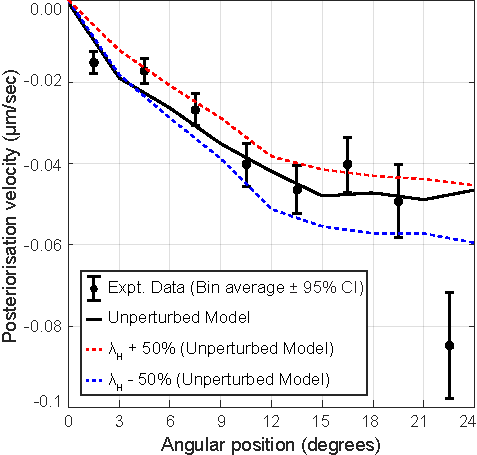
\includegraphics[width=\textwidth]{Results/FigComparePCF/wtPostVelModelLhVary.pdf}
        \caption{Varying \hydrodynamicLength between [\SI{5}{\unitLength},\SI{15}{\unitLength}]. Increasing \hydrodynamicLength leads to slower posteriorisation velocity.}
        \label{subfig:unperturbedModelParameterVary-Lh}
    \end{subfigure}
    \hfill
    \begin{subfigure}[t]{0.45\textwidth}
        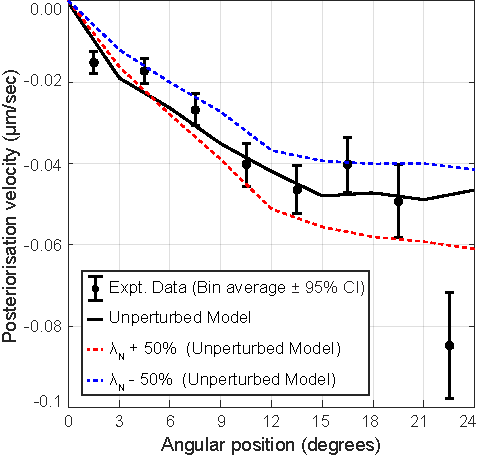
\includegraphics[width=\textwidth]{Results/FigComparePCF/wtPostVelModelLnVary.pdf}
        \caption{Varying \nematicLength between [\SI{76.25}{\unitLength},\SI{228.75}{\unitLength}]. Increasing \nematicLength leads to faster posteriorisation velocity.}
        \label{subfig:unperturbedModelParameterVary-Ln}
    \end{subfigure}
    \caption[Effect of model parameter variation on calculated posteriorisation velocity]{Posteriorisation velocity of the male pronucleus calculated by the unperturbed model (theoretical model evaluated with model parameters: \hydrodynamicLength = \SI{10}{\unitLength}, \activeRelaxLength = \SI{11.5}{\square\unitLength\per\second}, \nematicLength = \SI{152.5}{\square\unitLength\per\second}, \dragCoefficient = \num{0.61}) is robust to variation in \hydrodynamicLength and \nematicLength. Comparison of the calculated posteriorisation velocity using calibrated model parameters (black line), calculated posteriorisation velocity with \hydrodynamicLength $\coloneqq$ \num{1.5}\hydrodynamicLength (\autoref{subfig:unperturbedModelParameterVary-Lh}, red dashed line) or \nematicLength $\coloneqq$ \num{1.5}\nematicLength (\autoref{subfig:unperturbedModelParameterVary-Ln}, red dashed line), calculated posteriorisation velocity with \hydrodynamicLength $\coloneqq$ \num{1.5}\hydrodynamicLength (\autoref{subfig:unperturbedModelParameterVary-Lh}, blue dashed line) or \nematicLength $\coloneqq$ \num{0.5}\nematicLength (\autoref{subfig:unperturbedModelParameterVary-Ln}, blue dashed line), and average posteriorisation velocity observed in unperturbed embryos (black circles with error bars, \num{95}\% confidence interval). Posteriorisation velocity is plotted on the y-axis in \si{\unitPostVel} against angular position on the x-axis in \si{\unitAngle}.}
    \label{fig:unperturbedModelParameterVary}
\end{figure}

Therefore, the full model (with both mechanisms included) can -- both qualitatively and quantitatively -- recapitulate the observed \ac{ap} axis alignment process in the unperturbed embryos, using the set of model parameters selected here: \hydrodynamicLength = \SI{10}{\unitLength}, \activeRelaxLength = \SI{11.5}{\square\unitLength\per\second}, \nematicLength = \SI{152.5}{\square\unitLength\per\second}, \dragCoefficient = \num{0.61}. The model evaluated with this set of model parameters will be referred to as the unperturbed model.

\FloatBarrier
\subsubsection{Eliminating role of pseudocleavage furrow-dependent mechanism in model explains the slower \acs{ap} axis alignment in pseudocleavage furrow-deficient embryos}\label{subsubsec:cytoModelForNop1Mel11}

Next, the theoretical model is compared with observations in the pseudocleavage furrow-deficient embryos generated by \geneExp{nop-1; mel-11} double \ac{rnai}. To mimic the experimental removal of the pseudocleavage furrow in the model, \nematicLength -- the model parameter that controls the contribution of the pseudocleavage-furrow dependent mechanism in the model (see \autoref{subsec:numericsModelMN}) -- is fixed to \SI{0}{\square\unitLength\per\second}. Due to this, and since the cortical flows in these embryos are similar but not identical to those observed in unperturbed embryos, the model is recalibrated to ensure cortical flows observed in the \geneExp{nop-1; mel-11} \ac{rnai} embryos are captured by the model. In this recalibration, only \activeRelaxLength is varied. Doing so yields the following model parameters: \hydrodynamicLength = \SI{10}{\unitLength}, \activeRelaxLength = \SI{7}{\square\unitLength\per\second}, \nematicLength = \SI{0}{\square\unitLength\per\second}. The value for the drag coefficient \dragCoefficient = \num{0.61} as determined for the unperturbed embryos is retained here. The model evaluated with this set of model parameters will be referred to as the pseudocleavage furrow-deficient model.

\begin{figure}
    \centering
    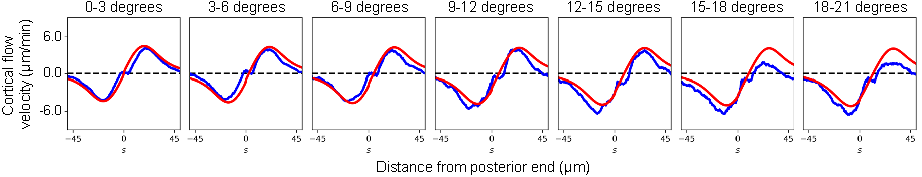
\includegraphics[width=\textwidth]{Results/FigComparePCF/nopMelCorticalFlowModel.pdf}
    \caption[Calibrating theoretical model using cortical flows observed in pseudocleavage furrow-deficient embryos]{Comparison of observed cortical flows in pseudocleavage furrow-deficient embryos generated using \geneExp{nop-1; mel-11} \ac{rnai} in SWG070 strain to those calculated by the theoretical model of \ac{ap} axis alignment, with setting \nematicLength = \SI{0}{\square\unitLength\per\second}. Blue line denotes the average cortical flow velocity observed in \geneExp{nop-1; mel-11} \ac{rnai} embryos, plotted as a function of position along the cortex $s$ in each angular position bin -- also depicted in \autoref{fig:resultsCorticalAvgFlowVsAngle}. Red denotes the cortical flow velocity calculated by the theoretical model after calibration, with model parameters: \hydrodynamicLength = \SI{10}{\unitLength}, \activeRelaxLength = \SI{7}{\square\unitLength\per\second}, \nematicLength = \SI{0}{\square\unitLength\per\second}.}
    \label{fig:pcfRemovedModelCalibrationCorticalFlows}
\end{figure}

Before a comparison with experimental data is made, the posteriorisation velocity calculated using the unperturbed model and the pseudocleavage-deficient model are compared (compare \autoref{subfig:pcfRemoveModelCompareExpt-postVel} with \autoref{subfig:unperturbedModelCompareExpt-postVel}). At each angular position, the pseudocleavage furrow-deficient model calculates slower posteriorisation velocity compared to the unperturbed model -- with the difference larger for higher angular positions. This is qualitatively similar to what was observed experimentally observed -- pseudocleavage furrow-deficient embryos (generated using \geneExp{nop-1; mel-11} \ac{rnai}) exhibit slower average posteriorisation velocities compared to unperturbed embryos at all angular positions observed in experiments -- with larger difference at higher angular positions (compare \autoref{fig:swg070WtPostVelVsAngle} to \autoref{fig:swg070Nop1Mel11PostVelVsAngle}). Direct comparison between the calculated posteriorisation velocity from the pseudocleavage furrow-deficient embryo to the experimental posteriorisation velocity observed in pseudocleavage furrow-deficient embryos (generated using \geneExp{nop-1; mel-11} \ac{rnai}) reveals that the calculated posteriorisation velocity broadly match the experimentally observed ones in the pseudocleavage furrow-deficient embryos -- see \autoref{subfig:pcfRemoveModelCompareExpt-postVel} and \autoref{tab:resultsPostVelNop1Mel11VsPcfRemoveModel}. Specifically, the pseudocleavage furrow-deficient model calculates posteriorisation velocity which are slightly slower, but still comparable to those observed in the pseudocleavage furrow-deficient embryos. As before, the calculated posteriorisation velocity may be integrated over to obtain a calculated trajectory of the male pronucleus using the pseudocleavage furrow-deficient model (see \autoref{subsec:numericsModelMN}). Comparison with experimentally observed trajectories in the pseudocleavage furrow-deficient embryo shows that the calculated trajectory agrees well with the experimentally observed trajectories of the male pronucleus observed in pseudocleavage furrow-deficient embryos -- see \autoref{subfig:pcfRemoveModelCompareExpt-tracks}.

\begin{table}
    \centering
    \begin{tabular}{|C{0.2\textwidth}|C{0.35\textwidth}|C{0.35\textwidth}|}
        \hline
        Angular positions (\si{\unitAngle}) & Experimental post. velocity (\SI{1e-1}{\unitPostVel}) & Calculated post. velocity (\SI{1e-1}{\unitPostVel})\\
        \hline
        \numrange{0}{3} & \num{-0.10} (\num{-0.12},\num{-0.08}) & \num{-0.03}\\
        \numrange{3}{6} & \num{-0.14} (\num{-0.17},\num{-0.11}) & \num{-0.07}\\
        \numrange{6}{9} & \num{-0.14} (\num{-0.17},\num{-0.11}) & \num{-0.08}\\
        \numrange{9}{12} & \num{-0.17} (\num{-0.21},\num{-0.13}) & \num{-0.11}\\
        \numrange{12}{15} & \num{-0.17} (\num{-0.21},\num{-0.13}) & \num{-0.12}\\
        \numrange{15}{18} & \num{-0.20} (\num{-0.25},\num{-0.16}) & \num{-0.12}\\
        \numrange{18}{21} & \num{-0.20} (\num{-0.25},\num{-0.16}) & \num{-0.12}\\
        \numrange{21}{24} & \num{-0.36} (\num{-0.44},\num{-0.29}) & \num{-0.11}\\
        \hline
    \end{tabular}
    \caption{Experimentally observed posteriorisation velocity for each angular position bin in pseudocleavage furrow-deficient embryos generated using \geneExp{nop-1; mel-11} \ac{rnai} compared with those calculated by the pseudocleavage furrow-deficient model (theoretical model evaluated with model parameters: \hydrodynamicLength = \SI{10}{\unitLength}, \activeRelaxLength = \SI{7}{\square\unitLength\per\second}, \nematicLength = \SI{0}{\square\unitLength\per\second}, \dragCoefficient = \num{0.61}). Experimental Post. velocity: Average posteriorisation velocity along with \num{95}\% confidence interval for each angular position bin observed in \geneExp{nop-1; mel-11} \ac{rnai} embryos (see \autoref{tab:resultsPostVelNop1Mel11} and \autoref{fig:swg070Nop1Mel11PostVelVsAngle}. Calculated Post. velocity: Posteriorisation velocity calculated at center of angular position bin by theoretical model with model parameters: \hydrodynamicLength = \SI{10}{\unitLength}, \activeRelaxLength = \SI{7}{\square\unitLength\per\second}, \nematicLength = \SI{0}{\square\unitLength\per\second}, \dragCoefficient = \num{0.61}.}
    \label{tab:resultsPostVelNop1Mel11VsPcfRemoveModel}
\end{table}

\begin{figure}
    \centering
    \begin{subfigure}[t]{0.45\textwidth}
        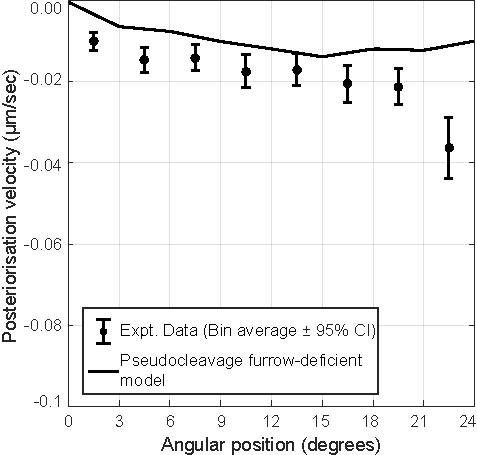
\includegraphics[width=\textwidth]{Results/FigComparePCF/nopMelPostVelModel.pdf}
        \caption{Comparing average posteriorisation velocity of the male pronucleus (black circles with error bars, \num{95}\% confidence interval) in pseudocleavage furrow-deficient embryos (from \autoref{fig:swg070Nop1Mel11PostVelVsAngle}) with that calculated by pseudocleavage furrow-deficient model (black line), both plotted against angular position of the male pronucleus. Posteriorisation velocity is on y-axis (in \si{\unitPostVel}, negative velocity indicate movement towards posterior end), and angular position on x-axis (in \si{\unitAngle}).}
        \label{subfig:pcfRemoveModelCompareExpt-postVel}
    \end{subfigure}
    \hfill
    \begin{subfigure}[t]{0.45\textwidth}
        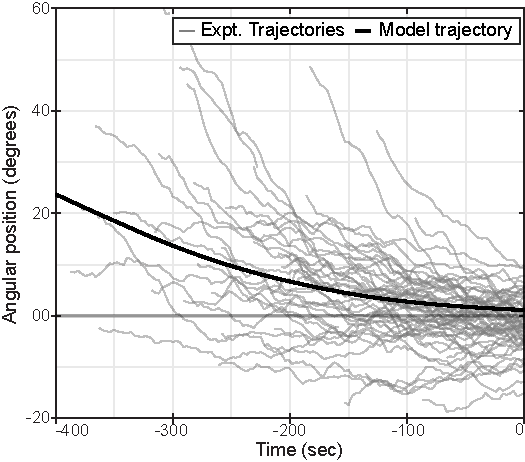
\includegraphics[width=\textwidth]{Results/FigComparePCF/wtTrajectoriesModel.pdf}
        \caption{Comparing angular positions of the male pronucleus (y-axis, in \si{\unitAngle}) observed in pseudocleavage furrow-deficient embryos (thin grey lines, from \autoref{fig:swg070Nop1Mel11Trajectories}) with the calculated trajectory of the male pronucleus (thick black line) from pseudocleavage furrow-deficient model, both plotted against time (on x-axis, in \si{\second}, t = \SI{0}{\second} denotes end of posteriorisation).}
        \label{subfig:pcfRemoveModelCompareExpt-tracks}
    \end{subfigure}
    \caption[Experimentally observed posteriorisation in pseudocleavage furrow-deficient embryos compared with that calculated by theoretical model]{Comparing experimentally observed posteriorisation of the male pronucleus in pseudocleavage furrow-deficient embryos generated by \geneExp{nop-1; mel-11} \ac{rnai} in SWG070 strain with that calculated by the pseudocleavage furrow-deficient model. Pseudocleavage furrow-deficient model refers to the theoretical model of \ac{ap} axis alignment evaluated with the following model parameters: \hydrodynamicLength = \SI{10}{\unitLength}, \activeRelaxLength = \SI{7}{\square\unitLength\per\second}, \nematicLength = \SI{0}{\square\unitLength\per\second}, \dragCoefficient = \num{0.61}.}
    \label{fig:pcfRemoveModelCompareExpt}
\end{figure} 

Therefore, the pseudocleavage furrow-deficient model -- where \nematicLength is set to \SI{0}{\square\unitLength\per\second} -- can recapitulate the observed \ac{ap} axis alignment process in the pseudocleavage furrow-deficient embryos generated using \geneExp{nop-1; mel-11} \ac{rnai} embryos. The pseudocleavage furrow-deficient model here refers to theoretical model evaluated with the following model parameters: \hydrodynamicLength = \SI{10}{\unitLength}, \activeRelaxLength = \SI{7}{\square\unitLength\per\second}, \nematicLength = \SI{0}{\square\unitLength\per\second}, \dragCoefficient = \num{0.61}.

%Note that pseudocleavage furrow is set to zero in model. Cortical flow calibration for nop-1/mel-11 embryos. Why do again calibration: because cortical flows are similar but not same. Show parameters. Comparison for posteriorization velocity and angular position with theory results - in that order. Conclusion: similar order, seems to capture behaviour.
%\subsubsection{Suppressed pseudocleavage furrow-dependent mechanism better explains \acs{ap} axis alignment in pseudocleavage furrow-deficient embryos}\label{subsubsec:reducedPcModelForNop1Mel11}
%We have reduced the expression of \geneExp{nop-1} (via \ac{rnai}) in order to generate pseudocleavage furrow-deficient embryos. Given that the pseudocleavage furrow-dependent mechanism arises due to the nematic nature of the cortex (see \autoref{ch:ActiveMatter}), we look into the effect \geneExp{nop-1} \ac{rnai} has on nematic order in the cortex. \ac{rnai} of \geneExp{nop-1} reduces the nematic order of the cortex, as measured in \cite{reymann2016cortical} by characterising the orientation of actin filaments. However, note that the cortex in these embryos still retains a weak nematic nature.

%Motivated by this observation, we ask if recalibrating the model for the pseudocleavage furrow-deficient embryos generated using \geneExp{nop-1; mel-11} \ac{rnai} while allowing \nematicLength to be non-zero would help explain the discrepancy between the experimentally observed average posteriorisation velocity in the double \ac{rnai} embryos and calculated posteriorisation velocity from the pseudocleavage furrow-deficient embryos. We thus recalibrate the model using the cortical flows experimentally observed in pseudocleavage furrow-deficient embryos , and allowing \nematicLength to vary during the recalibration. We still retain the drag coefficient \dragCoefficient = \num{0.61} -- same as used for the unperturbed model. Doing so yields the following model parameters: \hydrodynamicLength = \SI{11}{\unitLength}, \activeRelaxLength = \SI{7}{\square\unitLength\per\second}, \nematicLength = \SI{25}{\square\unitLength\per\second}. We will refer to the model evaluated with this set of model parameters as the weak pseudocleavage furrow model. Note that the change in \nematicLength between the pseudocleavage furrow-deficient model and the weak pseudocleavage furrow model is much smaller ($\sim$\num{20}\%) compared to the difference between the pseudocleavage furrow-deficient model and the unperturbed model. 

%We then compare the posteriorisation velocity calculated by the weak pseudocleavage furrow model with the experimentally observed average posteriorisation velocity in pseudocleavage furrow-deficient embryos (generated using \geneExp{nop-1; mel-11} \ac{rnai}). We find that the calculated posteriorisation velocity using the weak pseudocleavage furrow model better match the experimentally observed average posteriorisation velocity in the pseudocleavage furrow-deficient embryos than those calculated by the pseudocleavage furrow-deficient model. Note however that the difference between the posteriorisation velocities calculated using the pseudocleavage furrow-deficient model and the weak pseudocleavage furrow model is much smaller than between either and those calculated using the unperturbed model.

\FloatBarrier
\subsubsection{Pseudocleavage furrow-dependent mechanism is the predominant mechanism for \acs{ap} axis alignment in unperturbed embryos}\label{subsubsec:pcFurrowDominatesConclude}

A further comparison between the experimentally observed posteriorisation velocity in the unperturbed embryos and pseudocleavage furrow-deficient embryos generated using \geneExp{nop-1; mel-11} \ac{rnai} embryos may now be made, by the plotting the two against each other. Specifically, the average posteriorisation velocities observed in a given angular position bin in the pseudocleavage furrow-deficient embryos are plotted against average posteriorisation velocities observed in the same angular position bin in the unperturbed embryos. Using this plot, the difference in the posteriorisation velocity between the two conditions at different angular positions may be visualized -- see \autoref{subfig:compareUnperturbedPcfRemove-expt}. A linear fit to this plot captures the trend observed in this plot, yielding a slope of $m = \num{0.34}$ -- implying that the average posteriorisation velocity observed in unperturbed embryos are about $\frac{1}{m} = \num{2.95}$ times faster than those observed in the pseudocleavage furrow-deficient embryos. 

Such a comparison may also made between the calculated posteriorisation velocity using the unperturbed model and the pseudocleavage furrow-deficient model, by plotting the calculated posteriorisation velocity from the pseudocleavage furrow-deficient model at a given angular position against the calculated posteriorisation velocity from the unperturbed model at the same angular position -- see \autoref{subfig:compareUnperturbedPcfRemove-model}. A linear fit to this plot yields a slope of $m = \num{0.23}$ -- implying that the posteriorisation velocity calculated by the unperturbed model are about $\frac{1}{m} = \num{4.39}$ times faster than those calculated by the pseudocleavage furrow-deficient model. Note that this factor is larger than that observed in the comparison of experimental posteriorisation velocities -- such a discrepancy could be explained by the slightly slower posteriorisation velocity calculated by the pseudocleavage furrow-deficient model compared to those observed in the pseudocleavage furrow-deficient \geneExp{nop-1; mel-11} \ac{rnai} embryos.

\begin{figure}
    \centering
    \begin{subfigure}[t]{0.45\textwidth}
        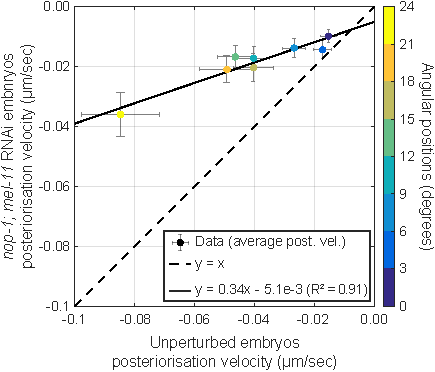
\includegraphics[width=\textwidth]{Results/FigComparePCF/compareExpt.pdf}
        \caption{Plotting average posteriorisation velocity (in \si{\unitPostVel}) observed in \geneExp{nop-1; mel-11} embryos (on y-axis) with those observed in the unperturbed embryos (on x-axis) at the same angular position bin -- see \autoref{fig:swg070Nop1Mel11PostVelVsAngle} and \autoref{fig:swg070WtPostVelVsAngle}.}
        \label{subfig:compareUnperturbedPcfRemove-expt}
    \end{subfigure}
    \hfill
    \begin{subfigure}[t]{0.45\textwidth}
        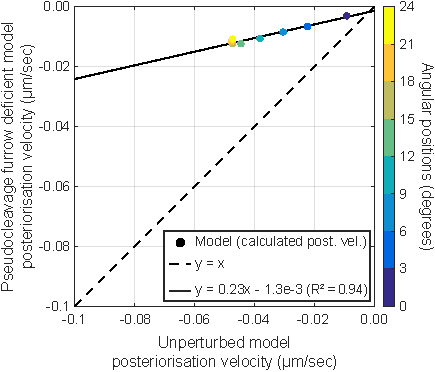
\includegraphics[width=\textwidth]{Results/FigComparePCF/compareModel.pdf}
        \caption{Plotting calculated posteriorisation velocity (in \si{\unitPostVel}) from the pseudocleavage furrow-deficient model (on y-axis) with those calculated using the unperturbed model (on x-axis) at the same angular position bin -- see \autoref{fig:pcfRemoveModelCompareExpt} and \autoref{fig:unperturbedModelCompareExpt}.}
        \label{subfig:compareUnperturbedPcfRemove-model}
    \end{subfigure}
    \caption[Experimentally observed posteriorisation in pseudocleavage furrow-deficient embryos compared with that calculated by theoretical model]{Comparing pseudocleavage deficient condition with pseudocleavage present/unperturbed condition using experiments (\autoref{subfig:compareUnperturbedPcfRemove-expt}) and theoretical model (\autoref{subfig:compareUnperturbedPcfRemove-model}). Color represents angular position bin for each datapoint. Dotted line indicates the $y = x$ line -- the line along which the datapoints would lie if the posteriorisation velocities were similar at all angular positions. Black line is the fitted line $y = m x + c$ for the data scatter. In \autoref{subfig:compareUnperturbedPcfRemove-expt}, error bars indicate the \num{95}\% confidence interval for the averages in both x- and y- axes.}
    \label{fig:compareUnperturbedPcfRemove}
\end{figure} 

\begin{table}
    \centering
    \begin{tabular}{|*{2}{C{0.14\textwidth}|}*{6}{C{0.09\textwidth}|}}
        \hline
        Model name & Compared to Expt. & \multicolumn{4}{c|}{Model parameters} & \multicolumn{2}{c|}{Ellipsoid}\\
        \cline{3-8}
        & & \hydrodynamicLength (\si{\unitLength}) & \activeRelaxLength (\si{\square\unitLength\per\second}) & \nematicLength (\si{\square\unitLength\per\second}) & \dragCoefficient & \longAxisLength (\si{\unitLength}) & \shortAxisLength (\si{\unitLength})\\
        \hline
        Unperturbed model & Unperturbed embryos & \num{10} & \num{11.5} & \num{152.5} & \num{0.61} & \num{28.9} & \num{16.4}\\
        \hline
        Pseudocleavage furrow-deficient model & \geneExp{nop-1; mel-11} \ac{rnai} embryos & \num{10} & \num{7} & \num{0} & \num{0.61} & \num{28.9} & \num{16.4}\\
        \hline
        Unperturbed model & \geneExp{ima-3} \ac{rnai} embryos & \num{10} & \num{11.5} & \num{152.5} & \num{0.61} & \num{25.7} & \num{17.3}\\
        \hline
    \end{tabular}
    \caption{Model parameters used for the theoretical model of \ac{ap} axis alignment for comparison with and/or prediction for different experimental conditions. Model name refers to the name of the evaluation of the theoretical model at the corresponding set of model parameters.}
    \label{tab:summaryModelParameters}
\end{table}

Therefore, the comparisons between the unperturbed embryos and pseudocleavage furrow-deficient embryos generated using \geneExp{nop-1; mel-11} \ac{rnai} demonstrate that the pseudocleavage furrow plays an important role in the substantially ($\sim 3$ times) faster dynamics of \ac{ap} axis alignment observed in unperturbed embryos, but is not essential to ensure \ac{ap} axis alignment occurs. Comparisons with numerical simulations using the theoretical model of \ac{ap} axis alignment described in \autoref{sec:apAxisAlignmentModelMN} show that \ac{ap} axis alignment in the two sets of embryos -- unperturbed embryos and pseudocleavage furrow-deficient embryos -- can be captured by the theoretical model, but with different model parameters \autoref{tab:summaryModelParameters}. Of note is \nematicLength, which changes the most between the two sets of model parameters (\nematicLength = \SI{152.5}{\square\unitLength\per\second} for unperturbed model and \nematicLength = \SI{0}{\square\unitLength\per\second} for pseudocleavage furrow-deficient model). This difference in the \nematicLength also indicates a substantially ($\sim 4$ times) faster dynamics in the unperturbed model compared to that calculated in the pseudocleavage furrow-deficient model. Note that \nematicLength is the model parameter that controls the contribution of the pseudocleavage furrow-dependent mechanism in the model (see \autoref{sec:apAxisAlignmentModelMN}). Altogether, these observations lead to the conclusion that the pseudocleavage furrow-dependent mechanism provides the major contribution to the posteriorisation velocity observed in the unperturbed embryos, and thus is the predominant mechanism responsible for the proper \ac{ap} axis alignment in the unperturbed embryos. Slow \ac{ap} axis alignment in the pseudocleavage-furrow deficient embryos indicates that the other mechanism -- the cytoplasmic flow-dependent mechanism -- plays a minor role in \ac{ap} axis alignment.

\FloatBarrier
\section{Role of embryo geometry in \acs{ap} axis alignment}\label{sec:GeometryRole}
Given that the \ac{ap} axis alignment process involves the alignment of the \ac{ap} axis -- defined by mechanochemical feedback between \ac{par} proteins and actomyosin cortex (see \autoref{sec:ApAxisEstablishment}) -- with the long axis of the embryo -- determined by its geometry -- a prime question to consider is the role of embryo geometry in \ac{ap} axis alignment, which is done in this section. Specifically, the difference in the rate of \ac{ap} axis alignment -- measured as the posteriorisation velocity of the male pronucleus -- between ellipsoidal embryos with differing aspect ratios is investigated. Aspect ratio of the embryo is defined as the ratio of the lengths of the long axis 2\longAxisLength and the two equal short axes 2\shortAxisLength~ -- aspect ratio = \aspectRatio.

\begin{table}
    \centering
    \begin{tabular}{|C{0.15\textwidth}|C{0.15\textwidth}|C{0.15\textwidth}|C{0.15\textwidth}|C{0.15\textwidth}|}
        \hline
        Experimental Condition & Strain & Semi-major axis ($a$, \si{\unitLength}) &  Semi-major axis ($b$, \si{\unitLength}) &  Aspect ratio ($\frac{a}{b}$)\\
        \hline
        Unperturbed & SWG070 & \num{28.9 +- 1.64} & \num{16.3 +- 1.17} & \num{1.78 +- 0.15}\\
        \geneExp{mlc-4} \ac{rnai} & SWG070 & \num{26.9 +- 1.50} & \num{15.4 +- 0.74} & \num{1.75 +- 0.08}\\
        \geneExp{nop-1} \ac{rnai} & SWG070 & \num{26.9 +- 2.12} & \num{17.11 +- 0.59} & \num{1.58 +- 0.12}\\
        \geneExp{nop-1; mel-11} \ac{rnai} & SWG070 & \num{26.4 +- 1.43} & \num{16.1 +- 0.96} & \num{1.64 +- 0.09}\\
        \geneExp{ima-3} \ac{rnai} & SWG070 & \num{22.0 +- 2.27} & \num{14.7 +- 1.20} & \num{1.48 +- 0.18}\\
        \geneExp{air-1} \ac{rnai} & SWG070 & \num{28.9 +- 1.36} & \num{15.6 +- 1.08} & \num{1.87 +- 0.14}\\
        Unperturbed & SWG057 & \num{27.4 +- 1.36} & \num{16.2 +- 0.89} & \num{1.70 +- 0.14}\\
        \geneExp{goa-1; gpa-16} \ac{rnai} & SWG057 & \num{26.9 +- 1.08} & \num{15.6 +- 1.13} & \num{1.74 +- 0.16}\\
        \hline
    \end{tabular}
    \caption{Quantification of embryo shape in various experimental conditions described in this thesis. Average value $\pm$ standard deviation are reported.}
    \label{tab:resultsEmbryoGeometry}
\end{table}

\subsection{Rounder embryos show slower \acs{ap} axis alignment}\label{subsec:roundEmbryosIma3}
Numerical simulations using the theoretical model described in \autoref{sec:apAxisAlignmentModelMN} are first used to investigate the influence of embryo geometry on \ac{ap} axis alignment. Specifically, the theoretical model is evaluated with the same model parameters as those used for the unperturbed embryos (that is, \hydrodynamicLength = \SI{10}{\unitLength}, \activeRelaxLength = \SI{11.5}{\square\unitLength\per\second}, \nematicLength = \SI{152.5}{\square\unitLength\per\second}, and \dragCoefficient = \num{0.61}), but on ellipsoids with different aspect ratios (\aspectRatio = \num{1.10}, \num{1.25}, \num{1.35}, \num{1.48}, \num{1.58}, \num{1.78}) which retain the same volume as that used for the unperturbed model. Note that \num{1.78} is the aspect ratio of the ellipsoid used for the unperturbed model -- corresponding to the average aspect ratio of unperturbed embryos (see \autoref{tab:resultsEmbryoGeometry}). For each aspect ratio, the theoretical model then predicts posteriorisation velocity of the male pronucleus as a function of its angular position (see \autoref{subsec:numericsModelMN}). Comparing the predictions for different aspect ratios, it is observed that the posteriorisation velocity at a given angular position are generally faster for higher aspect ratio -- \autoref{fig:numericalSimulationsAllAspectRatios}. This difference between posteriorisation velocity at different aspect ratios is larger at higher angular positions. Thus, the theoretical model predicts that the rate of \ac{ap} axis alignment is influenced by aspect ratio of the ellipsoid, and therefore embryo geometry -- with rounder embryos (that is, embryos with smaller aspect ratios) exhibiting slower \ac{ap} axis alignment compared to more ellipsoidal ones (that is, embryos with larger aspect ratios). Note that such a prediction is consistent with the extreme case of a perfectly round (or spherical) embryo; since such a spherical embryo lacks any unique long axis, no \ac{ap} axis alignment is expected in a spherical embryo.

\begin{figure}
\centering
\includegraphics[width=\textwidth]{Results/FigRoleGeometry/numSimAspRatio.pdf}
\caption[Theoretical model predicts slower posteriorisation for rounder embryos]{Posteriorisation velocity of the male pronucleus predicted by the theoretical model for embryos with different aspect ratios. Theoretical model is evaluated with the following model parameters: \hydrodynamicLength = \SI{10}{\unitLength}, \activeRelaxLength = \SI{11.5}{\square\unitLength\per\second}, \nematicLength = \SI{152.5}{\square\unitLength\per\second}, and \dragCoefficient = \num{0.61}), but on ellipsoids with different aspect ratios: \aspectRatio = \num{1.10}, \num{1.25}, \num{1.35}, \num{1.48}, \num{1.58}, \num{1.78}. Posteriorisation velocity is plotted on the y-axis (in \si{\unitPostVel}) against angular position of the male pronucleus on the x-axis (in \si{\unitAngle}).}
\label{fig:numericalSimulationsAllAspectRatios}
\end{figure}

To verify these predictions experimentally, embryos with aspect ratios smaller than those observed in unperturbed embryos were generated by performing a \ac{rnai} of \geneExp{ima-3} on worms of SWG070 strain for a feeding time of \SI{20}{\unitRNAiTime} (see \autoref{sec:rnaiMethods} for details on \ac{rnai}). IMA-3 is a member of the importin $\alpha$ family of nuclear transport factors \citep{geles2001germline,sonnichsen2005full}. It has been observed in previous studies that \geneExp{ima-3} \ac{rnai} generates rounder and smaller embryos \citep{sonnichsen2005full}. This observation is verified here by measuring the lengths of the semi-major \longAxisLength and semi-minor \shortAxisLength axes and the aspect ratio of \geneExp{ima-3} \ac{rnai} embryos and comparing them to those measured for the unperturbed embryos (see \autoref{subsec:nucleusTracking} for details). The average axes lengths for the unperturbed embryos were measured to be \longAxisLength = \SI{28.7 +- 1.6}{\unitLength} and \shortAxisLength = \SI{16.2 +- 1.1}{\unitLength}, corresponding to an aspect ratio of \aspectRatio = \num{1.78 +- 0.20}. This is compared to the average axes lengths and aspect ratio measured for \geneExp{ima-3} \ac{rnai} embryos, which were found to be \longAxisLength = \SI{20.9 +- 2.2}{\unitLength}, \shortAxisLength = \SI{13.8 +- 0.8}{\unitLength} and \aspectRatio = \num{1.48 +- 0.20}. It is also noted that the average volume (calculated for each embryo as the volume of the ellipsoid with the same axes lengths as those measured for the embryo) is smaller in \geneExp{ima-3} \ac{rnai} embryos compared to unperturbed embryos -- indicating \geneExp{ima-3} \ac{rnai} embryos have a smaller volume compared to unperturbed embryos -- see \autoref{fig:swg070Ima3CompareSwg070WtGeometry}. In summary, embryos generated using \geneExp{ima-3} \ac{rnai} were observed to be smaller and rounder compared to unperturbed embryos, on average.

\begin{figure}
\centering
\includegraphics[width=\textwidth]{Results/FigRoleGeometry/ima3Micrograph.pdf}
\caption[Representative micrograph: \geneExp{ima-3} \acs{rnai} embryos]{Representative \geneExp{ima-3} \acs{rnai} embryo of SWG070 strain, labelled with \flurophoreLabel{\ac{nmy2}}{\ac{gfp}} (white), showing the posteriorisation of the male pronucleus and the concurrent movement of the myosin depletion (indicating the \ac{ppar} domain) towards the posterior end. The male pronucleus can be visualized as the dark circle in the myosin channel towards the posterior end (right). T = \SI{0}{\second} is set at the end of posteriorisation of the male pronucleus. Scale bar: \SI{10}{\unitLength}. Images are rotated such that anterior and posterior ends are to the left and right respectively.}
\label{fig:swg070Ima3Micrograph}
\end{figure}

\begin{figure}
\centering
\begin{subfigure}[t]{0.3\textwidth}
    \centering
    \includegraphics[width=\textwidth]{Results/FigRoleGeometry/axesLengthsWtIma3.pdf}
    \caption{Comparing embryo axes lengths. p-value = \num{2.02e-18} for semi-major axis comparison, p-value = \num{4.22e-8} for semi-minor axis comparison.} 
    \label{subfig:swg070Ima3CompareSwg070WtGeometry-axesLength}
\end{subfigure}
\hfill
\begin{subfigure}[t]{0.3\textwidth}
    \centering
    \includegraphics[width=\textwidth]{Results/FigRoleGeometry/volWtIma3.pdf}
    \caption{Comparing embryo volumes. p-value = \num{1.59e-6}.} 
    \label{subfig:swg070Ima3CompareSwg070WtGeometry-volume}
\end{subfigure}
\hfill
\begin{subfigure}[t]{0.3\textwidth}
    \centering
    \includegraphics[width=\textwidth]{Results/FigRoleGeometry/aspRatioWtIma3.pdf}
    \caption{Comparing embryo aspect ratios. p-value = \num{1.48e-12}} 
    \label{subfig:swg070Ima3CompareSwg070WtGeometry-aspRatio}
\end{subfigure}
\caption[Comparing embryo geometry between unperturbed embryos and \geneExp{ima-3} \acs{rnai} embryos]{Comparison of embryo geometry between unperturbed embryos (N = 57, blue) and \geneExp{ima-3} \ac{rnai} embryos (N = 35, red), both from the SWG070 strain. Semi-major \longAxisLength and semi-minor \shortAxisLength axes lengths (\autoref{subfig:swg070Ima3CompareSwg070WtGeometry-axesLength}), volume (calculated using measured semi-major and semi-minor axis lengths, \autoref{subfig:swg070Ima3CompareSwg070WtGeometry-volume}) and aspect ratio (calculated using measured semi-major and semi-minor axis lengths, \autoref{subfig:swg070Ima3CompareSwg070WtGeometry-aspRatio}) are compared. Datapoints represent axes lengths, volume and aspect ratios measured for individual embryos in \autoref{subfig:swg070Ima3CompareSwg070WtGeometry-axesLength}, \autoref{subfig:swg070Ima3CompareSwg070WtGeometry-volume} and \autoref{subfig:swg070Ima3CompareSwg070WtGeometry-aspRatio} respectively. p-values are calculated using a two-sided t-test.}
\label{fig:swg070Ima3CompareSwg070WtGeometry}
\end{figure}

To ensure that the model parameters used in the unperturbed model can be used for comparison with \geneExp{ima-3} \ac{rnai} embryos, myosin concentrations in the cytosol and cortex were measured and compared between the \geneExp{ima-3} \ac{rnai} embryos and unperturbed embryos (see \autoref{subsec:nucleusTracking} for methods); alongwith cortical flows. Myosin concentrations in the cytosol were measured to be \SI{79.2 +- 4.3}{\unitMyosinConc} in \geneExp{ima-3} \ac{rnai} embryos, compared to \SI{80.9 +- 13.8}{\unitMyosinConc} in unperturbed embryos; myosin concentrations in the cortex were measured to be \SI{80.3 +- 4.7}{\unitMyosinConc} in \geneExp{ima-3} \ac{rnai} embryos, compared to \SI{76.2 +- 11.1}{\unitMyosinConc} in unperturbed embryos; and average cortical flow speeds in the cortex were measured to be \SI{3.99 +- 0.51}{\unitMyosinConc} in \geneExp{ima-3} \ac{rnai} embryos, compared to \SI{4.12 +- 0.59}{\unitMyosinConc} in unperturbed embryos. Thus, the \ac{ap} axis alignment process in the \geneExp{ima-3} \ac{rnai} embryos may be assumed to differ from that observed in the unperturbed embryos due to the difference in embryo geometry between the two sets of embryos -- see \autoref{fig:swg070Ima3CompareSwg070WtCortex}. Thus, the same model parameters as those used in the unperturbed model can be used for comparison with the rounder  \geneExp{ima-3} \ac{rnai} embryos.

\begin{figure}
\centering
\begin{subfigure}[t]{0.3\textwidth}
    \centering
    \includegraphics[width=\textwidth]{Results/FigRoleGeometry/crtxSpeedWtIma3.pdf}
    \caption{Comparing average cortical speeds in embryos. p-value = \num{0.28}} 
    \label{subfig:swg070Ima3CompareSwg070WtCortex-speed}
\end{subfigure}
\begin{subfigure}[t]{0.3\textwidth}
    \centering
    \includegraphics[width=\textwidth]{Results/FigRoleGeometry/myosinConcWtIma3.pdf}
    \caption{Comparing myosin concentrations in embryos. p-value = \num{0.72} for myosin concentration in cortex, p-value = \num{0.19} for myosin concentration in cytosol.} 
    \label{subfig:swg070Ima3CompareSwg070WtCortex-myosinConc}
\end{subfigure}
\caption[Comparing myosin concentrations and cortex flow speeds between unperturbed embryos and \geneExp{ima-3} \acs{rnai} embryos]{Comparison of myosin concentrations and cortex flow speeds between unperturbed embryos (N = 57, blue) and \geneExp{ima-3} \ac{rnai} embryos (N = 35, red), both from the SWG070 strain. Average cortical flow speeds (\autoref{subfig:swg070Ima3CompareSwg070WtCortex-speed}) and myosin concentrations in the cytosol and cortex (\autoref{subfig:swg070Ima3CompareSwg070WtCortex-myosinConc}, see \autoref{subsec:nucleusTracking}) are compared. Datapoints represent average cortical flow speeds, myosin concentration in cytosol and cortex measured for individual embryos in \autoref{subfig:swg070Ima3CompareSwg070WtCortex-speed} and \autoref{subfig:swg070Ima3CompareSwg070WtCortex-myosinConc} respectively. Myosin concentration is estimated as the average intensity of \flurophoreLabel{\ac{nmy2}}{\ac{gfp}} per pixel in
the cortex and cytosol. Intensity of \flurophoreLabel{\ac{nmy2}}{\ac{gfp}} are measured in arbitrary units (\si{AU}). p-values are calculated using a two-sided t-test.}
\label{fig:swg070Ima3CompareSwg070WtCortex}
\end{figure}

To obtain the predicted posteriorisation velocity observed in rounder \geneExp{ima-3} \ac{rnai} embryos, the theoretical model is therefore evaluated on the following model parameters: \hydrodynamicLength = \SI{10}{\unitLength}, \activeRelaxLength = \SI{11.5}{\square\unitLength\per\second}, \nematicLength = \SI{152.5}{\square\unitLength\per\second}, and \dragCoefficient = \num{0.61}, on an ellipsoid with semi-major axis \longAxisLength = \SI{25.7}{\unitLength} and semi-minor axes \shortAxisLength = \SI{17.3}{\unitLength}. Note that this yields an ellipsoid with aspect ratio \aspectRatio = \num{1.48} that matches the average aspect ratio observed in the \geneExp{ima-3} \ac{rnai} embryos, but with the same volume as that observed in unperturbed embryos -- therefore, the model prediction neglects the difference in volume between the \geneExp{ima-3} \ac{rnai} embryos and unperturbed embryos. On comparison of the predicted posteriorisation velocity with the experimentally measured posteriorisation velocity in the \geneExp{ima-3} \ac{rnai} embryos as a function of angular position (see \autoref{subfig:ima3ModelCompareExpt-postVel}), it is observed that predicted posteriorisation velocity agree with experimentally observed average posteriorisation velocity in \ac{rnai} embryos, for angular positions upto \SI{24}{\unitAngle}. For higher angular positions, average posteriorisation velocity observed in experiments is faster compared to predicted posteriorisation velocity for the same angular position. By integrating the predicted posteriorisation velocity as a function of angular position (see \autoref{subsec:numericsModelMN}), a predicted trajectory of the male pronucleus in the rounder \geneExp{ima-3} \ac{rnai} embryos is obtained, which agrees well with the experimentally observed trajectories of the male pronucleus in the \geneExp{ima-3} \ac{rnai} embryos -- see \autoref{subfig:ima3ModelCompareExpt-tracks}.

A direct comparison of the posteriorisation of the male pronucleus observed in \geneExp{ima-3} \ac{rnai} embryos and unperturbed embryos is also made. Average posteriorisation velocity in each angular position bins observed in the rounder \geneExp{ima-3} \ac{rnai} embryos were slower than those observed in the unperturbed embryos at the same angular position bins --  with larger differences for higher angular positions (compare \autoref{fig:swg070Ima3PostVelVsAngle} to \autoref{fig:swg070WtPostVelVsAngle}). As with unperturbed embryos, the angular positions were observed to decrease towards \SI{0}{\unitAngle} in the rounder \geneExp{ima-3} \ac{rnai} embryos -- see \autoref{fig:swg070Ima3Trajectories}. Fitting an exponential $\alpha = \alpha_0 + \exp(\frac{t}{t_0})$ to the angular positions observed in \geneExp{ima-3} \ac{rnai} embryos yields a time constant $t_0 = \SI{133 +- 3}{\second}$ and $\alpha_0 = \SI{1.68 +- 0.29}{\unitAngle}$. Note that the time constant obtained for \geneExp{ima-3} \ac{rnai} embryos ($t_0 = \SI{133 +- 3}{\second}$) is larger than that obtained for unperturbed embryos ($t_0 = \SI{118 +- 3}{\second}$). Altogether, these observations lead to the conclusion that the rounder \geneExp{ima-3} \ac{rnai} embryos exhibit a slower rate of \ac{ap} axis alignment compared to unperturbed embryos -- matching the prediction of the theoretical model. Note also that while the posteriorisation velocity is slower in \geneExp{ima-3} \ac{rnai} embryos compared to those observed in unperturbed embryos, but is faster than those observed in the pseudocleavage furrow-deficient embryos generated by the \geneExp{nop-1; mel-11} \ac{rnai} -- compare \autoref{fig:swg070Ima3Micrograph}, \autoref{fig:swg070WtPostVelVsAngle} and \autoref{fig:swg070Nop1Mel11PostVelVsAngle}.

\begin{figure}
\centering
\begin{subfigure}[t]{0.4\textwidth}
    \centering
    \includegraphics[width=\textwidth]{Results/FigRoleGeometry/ima3Trajectories.pdf}
    \caption{Trajectories of the male pronucleus (denoted by the coordinates of its center) observed in \geneExp{ima-3} \ac{rnai} embryos. Color represents time. x- and y-axes lie along the long and short axes of an ellipse with semi-major axis $a = \SI{22.0}{\unitLength}$ and semi-minor axis $b = \SI{14.7}{\unitLength}$. Scale bar: \SI{5}{\unitLength}} 
    \label{subfig:swg070Ima3Trajectories-tracks}
\end{subfigure}
\hfill
\begin{subfigure}[t]{0.57\textwidth}
    \centering
    \includegraphics[width=\textwidth]{Results/FigRoleGeometry/ima3Angular.pdf}
    \caption{Angular position of the male pronucleus (on y-axis, in \si{\unitAngle}) plotted as a function of time (on x-axis, in \si{\second}), in \geneExp{ima-3} \ac{rnai} embryos. Thin black lines represent individual trajectories, thick black line represents a exponential fit to the average of these tracks: $\alpha = \alpha_0 + \exp(-\frac{t}{t_0})$, with $t_0 = \SI{133 +- 3}{\second}$ and $\alpha_0 = \SI{1.68 +- 0.29}{\unitAngle}$.} 
    \label{subfig:swg070Ima3Trajectories-angleVsTime}
\end{subfigure}
\caption[Experimentally observed trajectories of the male pronucleus in \geneExp{ima-3} \acs{rnai} embryos]{Experimentally observed trajectories of the male pronucleus during posteriorisation in \geneExp{ima-3} \ac{rnai} embryos of SWG070 strain (N = 35). See \autoref{subsec:nucleusTracking} for details on male pronucleus tracking. Average semi-major and semi-minor axes lengths for \geneExp{ima-3} \ac{rnai} embryos of SWG070 strain are used in \autoref{subfig:swg070Ima3Trajectories-tracks} -- see \autoref{tab:resultsEmbryoGeometry}. Angular position is defined as the angle between the long axis and line connecting the centers of the male pronucleus and embryo. T = \SI{0}{\second} denotes end of posteriorisation.}
\label{fig:swg070Ima3Trajectories}
\end{figure}

\begin{figure}[p]
\centering
\includegraphics[width=0.95\textwidth]{Results/FigRoleGeometry/ima3PostVel.pdf}
\caption[Experimentally observed posteriorisation velocity of the male pronucleus in \geneExp{ima-3} \acs{rnai} embryos]{Top: Posteriorization velocity of the male pronucleus (along y-axis, in \si{\unitPostVel}) plotted against its angular position, in \geneExp{ima-3} \ac{rnai} embryos of SWG070 strain (N = 35). Negative values of the posteriorisation velocity indicate movement towards the posterior end. Angular position is binned using a bin width of \SI{3}{\unitAngle}. Black circles with errors bars denote the average posteriorization velocity with \num{95}\% confidence intervals in each angular position bin. Grey circles represent the data scatter -- the measured posteriorization velocities for different angular positions in each embryo (see \autoref{subsec:nucleusTracking}). Bottom: Histogram of the number of movies (along y-axis) contributing to each angular position (along x-axis) bin. A movie is considered to contribute to an angular position bin if it has any frames with angular positions within that bin. Note that a movie can contribute to multiple bins, as it may contain frames spanning different angular positions.}
\label{fig:swg070Ima3PostVelVsAngle}
\end{figure}

\begin{figure}
    \centering
    \begin{subfigure}[t]{0.45\textwidth}
        \includegraphics[width=\textwidth]{Results/FigRoleGeometry/ima3PostVelModelPredict.pdf}
        \caption{Comparing average posteriorisation velocity of the male pronucleus (black circles with error bars, \num{95}\% confidence interval) in \geneExp{ima-3} \ac{rnai} embryos (from \autoref{fig:swg070Ima3PostVelVsAngle}) with that predicted by unperturbed model on an ellipsoid with aspect ratio \aspectRatio = \num{1.48} (black line), both plotted against angular position of the male pronucleus. Posteriorisation velocity is on y-axis (in \si{\unitPostVel}, negative velocity indicate movement towards posterior end), and angular position on x-axis (in \si{\unitAngle}).}
        \label{subfig:ima3ModelCompareExpt-postVel}
    \end{subfigure}
    \hfill
    \begin{subfigure}[t]{0.45\textwidth}
        \includegraphics[width=\textwidth]{Results/FigRoleGeometry/ima3AngularModelPredict.pdf}
        \caption{Comparing angular positions of the male pronucleus (y-axis, in \si{\unitAngle}) observed in \geneExp{ima-3} \ac{rnai} embryos (thin grey lines, from \autoref{fig:swg070Ima3Trajectories}) with the predicted trajectory of the male pronucleus (thick black line) from unperturbed model on an ellipsoid with aspect ratio \aspectRatio = \num{1.48}, both plotted against time (on x-axis, in \si{\second}, t = \SI{0}{\second} denotes end of posteriorisation).}
        \label{subfig:ima3ModelCompareExpt-tracks}
    \end{subfigure}
    \caption[Experimentally observed posteriorisation in \geneExp{ima-3} \acs{rnai} embryos compared with that predicted by theoretical model]{Comparing experimentally observed posteriorisation of the male pronucleus in \geneExp{ima-3} \ac{rnai} embryos of the SWG070 strain with that predicted by the unperturbed model on an ellipsoid with aspect ratio \aspectRatio = \num{1.48}. Unperturbed model refers to the theoretical model of \ac{ap} axis alignment evaluated with the following model parameters: \hydrodynamicLength = \SI{10}{\unitLength}, \activeRelaxLength = \SI{11.5}{\square\unitLength\per\second}, \nematicLength = \SI{152.5}{\square\unitLength\per\second}, \dragCoefficient = \num{0.61}.}
    \label{fig:ima3ModelCompareExpt}
\end{figure} 

Altogether, these observations lead to the conclusion that rounder embryos do indeed show slower rate of \ac{ap} axis alignment -- as predicted by the theoretical model and confirmed experimentally. Since the diminished posteriorisation velocity observed in the rounder \geneExp{ima-3} \ac{rnai} embryos match the posteriorisation velocity predicted by the model using the same aspect ratio as the average aspect ratio observed in \geneExp{ima-3} \ac{rnai} embryos, the theoretical model captures this relation between embryo geometry and \ac{ap} axis alignment in a quantitative manner. Additionally, the prediction for the \geneExp{ima-3} \ac{rnai} embryos only takes into account the change in aspect ratio of the embryos, yet makes a prediction that matches the experimental observations -- implying that the primary feature of embryo geometry that influences \ac{ap} axis alignment is the aspect ratio of the embryo.

\FloatBarrier
\subsection{Relation between embryo geometry and \acs{ap} axis alignment}\label{subsec:postVelVsAspectRatio}

\subsubsection{Exploring the relation between aspect ratio and posteriorisation velocity}\label{subsubsec:postVelVsAspectRatioExpAndModel}
The predictions made using the theoretical model for embryos with different aspect ratios indicate a relation between the aspect ratio of the embryo and the rate of \ac{ap} axis alignment (measured as the posteriorisation velocity of the male pronucleus): slower rate of \ac{ap} axis alignment (that is, slower posteriorisation velocity at different angular positions) for smaller aspect ratios (that is, rounder embryos). To evaluate this relation experimentally, the following procedure is considered. Instead of considering the posteriorisation velocity of the male pronucleus as a function of angular position for a given average aspect ratio (as has been done until now), the posteriorization velocity are now considered as a function of aspect ratio, averaged over a range of angular positions. Experimental variation in the aspect ratios of both unperturbed (\numrange{1.6}{2.1}) and \geneExp{ima-3} \ac{rnai} embryos (\numrange{1.1}{1.7}) enables evaluating the relation between aspect ratio and posteriorisation velocity over a broad range of aspect ratios (\numrange{1.1}{2.1}) -- see \autoref{fig:swg070CombinedPostVelVsAspectRatio}. Since the difference in volume between the unperturbed embryos and \ac{rnai} embryos does not appear to be important for \ac{ap} axis alignment, and that cortical flows and myosin concentrations are not significantly different between unperturbed embryos and \geneExp{ima-3} \ac{rnai} embryos; these two sets of embryos can be combined into a single set which is now considered. In other words, the set of embryos considered in this subsection contains both the unperturbed embryos and \geneExp{ima-3} \ac{rnai} embryos, with no distinction made between the two. This set of embryos will be referred to as the combined set of embryos.

To obtain the experimentally observed relation between the posteriorisation velocity of the male pronucleus and aspect ratio of the embryo from the combined set of embryos, the combined set is binned using aspect ratio with a bin width of \num{0.2}. For each bin, the observed posteriorisation velocity included in this aspect ratio bin are averaged over all angular positions between \SIrange{3}{15}{\unitAngle}. This yields the average posteriorisation velocity (along with \num{95}\% confidence intervals calculated using two sided t-test) observed for each aspect ratio bin -- thus yielding the experimentally observed relation between the two -- see \autoref{fig:swg070CombinedPostVelVsAspectRatio}.

From the numerical simulations done using ellipsoids with different aspect ratios, a similar relation between the posteriorisation velocity and aspect ratio can be predicted by the theoretical model. For each aspect ratio used in numerical simulations described before, the posteriorisation velocity are averaged for all angular positions between \SIrange{3}{15}{\unitAngle}. For aspect ratios in-between, linear interpolation is utilised. This yields the relation between the posteriorisation velocity and aspect ratio, as predicted using the theoretical model -- see \autoref{fig:postVelVsAspectRatioAllModelsCompare}. Comparing to the experimentally observed relation, the predicted relation agrees with the experimentally obtained one over a range of aspect ratios from \numrange{1.1}{1.7}.

\begin{figure}[p]
\centering
\includegraphics[width=0.95\textwidth]{Results/FigRoleGeometry/postVelVsAspRatioData.pdf}
\caption[Posteriorisation velocity of the male pronucleus in unperturbed and \geneExp{ima-3} \acs{rnai} embryos with respect to aspect ratio]{Top: Posteriorization velocity of the male pronucleus (along y-axis, in \si{\unitPostVel}) plotted against aspect ratio of the embryo, in combined set embryos -- comprised of unperturbed embryos and \geneExp{ima-3} \ac{rnai} embryos. Negative values of the posteriorisation velocity indicate movement towards the posterior end. Aspect ratios is binned using a bin width of \num{0.2}. Black circles with errors bars denote the average posteriorization velocity with \num{95}\% confidence intervals in each aspect ratio bin. Grey circles represent the data scatter -- the measured posteriorization velocities for different aspect ratios in each embryo (see \autoref{subsec:nucleusTracking}). Bottom: Histogram of the frequency of movies (number of movies divided by total number of movies in the set, along y-axis) contributing to each aspect ratio (along x-axis) bin, for unperturbed embryos (blue) and \geneExp{ima-3} \ac{rnai} embryos (red).}
\label{fig:swg070CombinedPostVelVsAspectRatio}
\end{figure}

\subsubsection{Effective model of a contractile ring on an ellipsoid captures the relation between embryo geometry and \acs{ap} axis alignment}\label{subsubsec:effectiveModel}

How does this relation between the embryo geometry (characterised by aspect ratio) and \ac{ap} axis alignment (characterised by posteriorisation velocity) arise? As shown in \autoref{subsec:expVsTheoryPcFurrow}, the predominant mechanism for \ac{ap} axis alignment is the pseudocleavage furrow-dependent mechanism. The pseudocleavage furrow may effectively be considered as a contractile ring, rotating about the equator of an ellipsoid (representing the embryo) during \ac{ap} axis alignment. Can this effective model of a contractile ring on an ellipsoid be enough to capture the relation between aspect ratio of the embryo and posteriorisation velocity of the male pronucleus as observed in the combined set of embryos?

The effective model considers a fixed ellipsoid with one long axis (of length 2\longAxisLength) and two equal short axes (of length 2\shortAxisLength each) -- see \autoref{fig:schematicEffectiveModel}. The long axis of the embryo defines the x-axis, while the two short axes define the y- and z- axes. On this ellipsoid, a contractile ring is considered to represent the pseudocleavage furrow. The center of the ring and the center of the ellipsoid are coincident (at the origin of the coordinate system). This ring rotates about the z-axis, representing the rotation of the pseudocleavage furrow during \ac{ap} axis alignment. Thus, the contractile ring has only a sole degree of freedom: the angle $\alpha$ made between the normal to the plane of the contractile ring and the x-axis. Only small angles $\alpha$ are considered here (as angular positions between \SIrange{3}{15}{\unitAngle} only were considered for the experimentally obtained relation between aspect ration and posteriorisation velocity).

\begin{figure}
    \centering
    \includegraphics{Results/FigRoleGeometry/effectiveModelSchematic.pdf}
    \caption[Schematic of effective model of a contractile ring on an ellipsoid]{Schematic depicting effective model of a contractile ring (red ellipse) with fixed line tension ($T$) moving on an ellipsoid (black thick ellipse) with a long axis of length 2\longAxisLength and two short axes of length 2\shortAxisLength. x-axis is along the long axis of the ellipsoid. Both y- and z- axes are along the equal short axes of the ellipsoid (black dashed ellipse resides in the yz plane). The contractile ring is free to rotate about the z-axis (red block arrows), and its position is described by the angle $\alpha$ made between the plane of the contractile ring and the yz-plane. In the effective model, $\alpha$ also describes the angular position of the male pronucleus, considered to always be positioned along the normal to the plane of the contractile ring.}
    \label{fig:schematicEffectiveModel}
\end{figure}

The following assumptions are made in the effective model, with regards to the dynamics of the contractile ring:
\begin{itemize}
    \item The ring has a constant line tension $T$ - independent of both the orientation of the ring ($\alpha$) and the shape of the ellipsoid (\longAxisLength, \shortAxisLength). Here, $T$ has units of force.
    \item The frictional torque acting on the ring is controlled by a frictional coefficient $\gamma$, and is given by $\gamma\cdot\dot{\alpha}$
    \item No inertial terms in the momentum balance are considered: Torque generated by the ring is perfectly balanced by the torque generated by friction.
\end{itemize}                                                                             
Under the above assumptions, the aim of the effective model is to calculate $\dot{\alpha}$ as a function of \longAxisLength, \shortAxisLength and $\alpha$ -- for small angles $\alpha$. 

\paragraph{Motion of contractile ring}
Consider the mechanical energy stored in the contractile ring, which is given by:
\begin{equation} \label{eq:energyDef}
    E = TC(\alpha)
\end{equation}
where $C(\alpha)$ is the total circumference of the ring.

To calculate the circumference of the ring for any given $\alpha$, a description of the ring as an intersection of the ellipsoid with the plane in which the ring resides is written. This plane makes an angle of $\alpha$ with the yz plane, and passes through the origin. Thus, it can be described by the equation: $y = -x\cot\alpha$. The ellipsoid itself can be described as $\frac{x^2}{a^2} + \frac{y^2 + z^2}{b^2} = 1$. On taking the intersection of the ring plane with the ellipsoid, the equation describing the ring can be obtained:
\begin{align*}
    \textrm{Plane: }&y = -x\cot\alpha \\
    \textrm{Ellipsoid: }&\frac{x^2}{a^2} + \frac{y^2 + z^2}{b^2} = 1 \\
    \textrm{Intersection (Ellipse): }&\frac{x^2}{a^2} + \frac{x^2\cot^2\alpha + z^2}{b^2} = 1\\
    &\implies x^2\left(\frac{a^2\cot^2\alpha + b^2}{a^2b^2}\right) + \frac{z^2}{b^2} = 1; \quad y = -x\cot\alpha
\end{align*}
Define $A = \frac{ab}{\sqrt{a^2\cot^2\alpha + b^2}}$. Then, the equation in the intersection part above can be written as: $\frac{x^2}{A^2} + \frac{z^2}{b^2} = 1$ - a form similar to the canonical form for an ellipse. Calling the parametric angle for this ellipse $\phi$, the position vector describing the ring $\Vec{r}$ can be written as:
\begin{equation*}
    \Vec{r} = \left(A\cos\phi,-A\cot\alpha\cos\phi,b\sin\phi\right); \quad A = \frac{ab}{\sqrt{a^2\cot^2\alpha + b^2}}
\end{equation*}
where $\phi \in [-\pi,\pi)$.

Note that the ring is an ellipse in its plane - since the intersection of an ellipsoid and a plane must be an ellipse. This can also be seen by the form by $\norm{\Vec{r}}^2$:
\begin{equation*}
    \norm{\Vec{r}}^2 = A^2(1 + \cot^2\alpha)\cos^2\phi + b^2\sin^2\phi
\end{equation*}
indicating that the contractile ring is an ellipse with semi-major $a_{ring}$ and semi-minor $b_{ring}$ axes, given by:
\begin{align*}
    a_{ring} &= A\sqrt{1 + \cot^2\alpha} = \frac{ab}{\sqrt{a^2\cot^2\alpha + b^2}}\sqrt{1 + \cot^2\alpha^2} = \frac{ab}{\sqrt{a^2\cos^2\alpha + b^2\sin^2\alpha}}\\
    b_{ring} &= b \\
    e_{ring} &= \sqrt{1 - \left(\frac{b_{ring}}{a_{ring}}\right)^2} = \sqrt{1 - \frac{a^2\cos^2\alpha + b^2\sin^2\alpha}{a^2}} = \sqrt{\sin^2\alpha - \frac{b^2}{a^2}\sin^2\alpha} = \sin\alpha\sqrt{1 - \frac{b^2}{a^2}}
\end{align*}
where $e_{ring}$ is the eccentricity of the ellipse formed by the ring. Note that since the ring rotates about the yz plane (i.e. the plane with the two short axes), the short axis of the ring is just $b$.

The circumference of the ring is then given by the circumference of this ellipse. The formula for the circumference of an ellipse is:
\begin{equation} \label{eq:circum}
    C(\alpha) = 4a_{ring}\int_0^{\frac{\pi}{2}} \sqrt{1 - e_{ring}^2\sin^2\phi} \dd{\phi}
\end{equation}

\paragraph{Torque generated by contractile ring}
Using \eqref{eq:energyDef} and \eqref{eq:circum}, the mechanical energy of the contractile energy is then:
\begin{align*}
    E &= TC(\alpha) = 4Ta_{ring}\int_0^{\frac{\pi}{2}} \sqrt{1 - e_{ring}^2\sin^2\phi} \dd{\phi}\\
    &= 4T\frac{ab}{\sqrt{a^2\cos^2\alpha + b^2\sin^2\alpha}}\int_0^{\frac{\pi}{2}} \sqrt{1 - \left(1 - \frac{b^2}{a^2}\right)\sin^2\alpha\sin^2\phi} \dd{\phi}
\end{align*}

The torque $\tau$ can then be expressed as:
\begingroup
\allowdisplaybreaks
\begin{align*}
    \tau &= -\dv{E}{\alpha} = -4T\dv{\alpha}\left(\frac{ab}{\sqrt{a^2\cos^2\alpha + b^2\sin^2\alpha}}\int_0^{\frac{\pi}{2}} \sqrt{1 - \left(1 - \frac{b^2}{a^2}\right)\sin^2\alpha\sin^2\phi_{ring}} \dd{\phi_{ring}}\right)\\
    &= -4T\left[\frac{ab(a^2 - b^2)\cos\alpha\sin\alpha}{\left(a^2\cos^2\alpha + b^2\sin^2\alpha\right)^{\flatfrac{3}{2}}}\int_0^{\frac{\pi}{2}} \sqrt{1 - \left(1 - \frac{b^2}{a^2}\right)\sin^2\alpha\sin^2\phi_{ring}} \dd{\phi_{ring}}\right.\\
    &\left.\quad + \frac{ab}{\sqrt{a^2\cos^2\alpha + b^2\sin^2\alpha}}\int_0^{\frac{\pi}{2}} \frac{-\left(1 - \frac{b^2}{a^2}\right)\sin\alpha\cos\alpha\sin^2\phi_{ring}}{\sqrt{1 - \left(1 - \frac{b^2}{a^2}\right)\sin^2\alpha\sin^2\phi_{ring}}} \dd{\phi_{ring}}\right]\\
    &= -4T\frac{ab(a^2 - b^2)\sin\alpha\cos\alpha}{\sqrt{a^2\cos^2\alpha + b^2\sin^2\alpha}}\\
    &\times\int_0^{\frac{\pi}{2}}\left[\frac{1 - \left(1 - \frac{b^2}{a^2}\right)\sin^2\alpha\sin^2\phi_{ring}}{a^2\cos^2\alpha + b^2\sin^2\alpha}-\frac{\sin^2\phi_{ring}}{a^2}\right]\frac{1}{\sqrt{1 - \left(1 - \frac{b^2}{a^2}\right)\sin^2\alpha\sin^2\phi_{ring}}}\dd{\phi_{ring}}\\
    &= -4T\frac{ab(a^2 - b^2)\sin\alpha\cos\alpha}{a^2\sqrt{a^2\cos^2\alpha + b^2\sin^2\alpha}}\\
    &\times\int_0^{\frac{\pi}{2}}\left[\frac{a^2 - \left(a^2 - b^2\right)\sin^2\alpha\sin^2\phi_{ring}}{a^2\cos^2\alpha + b^2\sin^2\alpha}-\sin^2\phi_{ring}\right]\frac{1}{\sqrt{1 - \left(1 - \frac{b^2}{a^2}\right)\sin^2\alpha\sin^2\phi_{ring}}}\dd{\phi_{ring}}\\
    &= -4T\frac{ab(a^2 - b^2)\sin\alpha\cos\alpha}{a^2\sqrt{a^2\cos^2\alpha + b^2\sin^2\alpha}}\\
    &\times\int_0^{\frac{\pi}{2}}a^2\left[\frac{1 - \sin^2\phi_{ring}}{a^2\cos^2\alpha + b^2\sin^2\alpha}\right]\frac{1}{\sqrt{1 - \left(1 - \frac{b^2}{a^2}\right)\sin^2\alpha\sin^2\phi_{ring}}}\dd{\phi_{ring}}\\
    \implies \tau &= -4T\frac{ab(a^2 - b^2)\sin\alpha\cos\alpha}{\left(a^2\cos^2\alpha + b^2\sin^2\alpha\right)^{\flatfrac{3}{2}}}\int_0^{\frac{\pi}{2}}\frac{\cos^2\phi_{ring}}{\sqrt{1 - \left(1 - \frac{b^2}{a^2}\right)\sin^2\alpha\sin^2\phi_{ring}}}\dd{\phi_{ring}}
\end{align*}
\endgroup

Using the Taylor expansion around $\alpha = 0$, $\tau$ can be expanded to linear order in $\alpha$ as $\tau = \left.\tau\right|_{\alpha=0} + \left.\dv{\tau}{\alpha}\right|_{\alpha=0}\alpha + \mathcal{O}(\alpha^2)$. Note that on $\alpha = 0$, the torque also goes to zero. To obtain the linear order expansion, the derivative of the torque at $\alpha = 0$ is calculated:
\begin{align*}
    \left.\dv{\tau}{\alpha}\right|_{\alpha=0} &= -4T\left.\dv{\alpha}\left[\frac{ab(a^2 - b^2)\sin\alpha\cos\alpha}{\left(a^2\cos^2\alpha + b^2\sin^2\alpha\right)^{\flatfrac{3}{2}}}\int_0^{\frac{\pi}{2}}\frac{\cos^2\phi_{ring}}{\sqrt{1 - \left(1 - \frac{b^2}{a^2}\right)\sin^2\alpha\sin^2\phi_{ring}}}\dd{\phi_{ring}}\right]\right|_{\alpha = 0} \\
    &= -4T \left[\dv{\alpha}\left(\frac{ab(a^2 - b^2)\sin\alpha\cos\alpha}{\left(a^2\cos^2\alpha + b^2\sin^2\alpha\right)^{\flatfrac{3}{2}}}\right)_{\alpha=0}\int_0^{\frac{\pi}{2}}\frac{\cos^2\phi_{ring}}{\sqrt{1 - \left(1 - \frac{b^2}{a^2}\right)(0)\sin^2\phi_{ring}}}\dd{\phi_{ring}}\right.\\
    &\quad + \left.\frac{ab(a^2 - b^2)*0*1}{\left(a^2(1) + b^2(0)\right)^{\flatfrac{3}{2}}}\dv{\alpha}\left(\int_0^{\frac{\pi}{2}}\frac{\cos^2\phi_{ring}}{\sqrt{1 - \left(1 - \frac{b^2}{a^2}\right)\sin^2\alpha\sin^2\phi_{ring}}}\dd{\phi_{ring}}\right)_{\alpha=0}\right]\\
    &= -4T \left[\frac{ab(a^2 - b^2)}{\left(a^2*1 + b^2*0\right)^{\flatfrac{3}{2}}}\right] \int_0^{\frac{\pi}{2}}\cos^2\phi_{ring}\dd{\phi_{ring}} = -4T\frac{ab(a^2-b^2)}{a^3}\frac{\pi}{4}\\
    \implies \left.\dv{\tau}{\alpha}\right|_{\alpha=0} &= -\pi T b\left(1 - \frac{b^2}{a^2}\right)
\end{align*}

Thus, by Taylor expansion, the torque to linear order in $\alpha$ is:
\begin{equation} \label{eq:torque}
    \tau \approx \left.\dv{\tau}{\alpha}\right|_{\alpha=0}\alpha =  -\pi T b\left(1 - \frac{b^2}{a^2}\right)\alpha
\end{equation}

\paragraph{Torque balance for the contractile ring}
Per the assumption of negligible inertial terms and the form of friction experienced by the ring, the torque balance of the ring can be written as:
\begin{equation*}
    \tau - \gamma\cdot\dot{\alpha} = 0
\end{equation*}
Putting in the expression for $\tau$ obtained before:
\begin{equation} \label{eq:alphaDot}
    \dot{\alpha} \approx - \frac{\pi T}{\gamma} b\left[1 - \frac{b^2}{a^2}\right]\alpha
\end{equation}

\paragraph{Calculating posteriorization velocity of the male pronucleus}
To get the posteriorization velocity of the male pronucleus $v$, an additional assumption is made: the angular position of the male pronucleus is the same as the angle $\alpha$ itself -- see \autoref{fig:schematicEffectiveModel}. Effectively, the male pronucleus acts as if it is rigidly attached to the normal vector to the contractile ring. Then, the position of the male pronucleus is given by:
\begin{align*}
    \textrm{On ellipsoid:}\quad & \frac{x_{nucl}^2}{a^2} + \frac{y_{nucl}^2}{b^2} = 1\\
    \textrm{Angle with x-axis (long axis):}\quad & x_{nucl} = r_{nucl}\cos\alpha, \quad y_{nucl} = r_{nucl}\sin\alpha\\
    \implies \frac{r_{nucl}^2\cos^2\alpha}{a^2} + \frac{r_{nucl}^2\sin^2\alpha}{b^2} &= 1\\
    \implies r_{nucl} = \frac{ab}{\sqrt{a^2\sin^2\alpha + b^2\cos^2\alpha}}
\end{align*}

The posteriorization velocity of the male pronucleus is then given by (for small angles $\alpha$, velocity is almost parallel to the cortex, hence the full magnitude can be considered):
\begin{align*}
    v \approx \sqrt{\left(\dv{x_{nucl}}{t}\right)^2 + \left(\dv{y_{nucl}}{t}\right)^2} = \sqrt{\dot{r}_{nucl}^2 + r_{nucl}^2\dot{\alpha}^2} 
\end{align*}
For small angle $\alpha$, $r_{nucl} \approx a - \frac{a^3}{b^2}\alpha^2 + \mathcal{O}(\alpha^3)$ and $\dot{r}_{nucl} = -2\frac{a^3}{b^2}\alpha\dot{\alpha} + \mathcal{O}(\alpha^2)$. Thus,
\begin{equation*}
    v = \sqrt{\dot{r}_{nucl}^2 + r_{nucl}^2\dot{\alpha}^2} = \dot{\alpha}\sqrt{a^2 - 2\frac{a^4}{b^2}\alpha^2 + 4\frac{a^6}{b^4}\alpha^2 + \mathcal{O}(\alpha^3)} = \dot{\alpha}\left(a + \mathcal{O}(\alpha^2)\right)
\end{equation*}

Therefore, using \eqref{eq:alphaDot}, the following expression for the posteriorisation velocity $v$, to linear order in the angular position $\alpha$, is obtained:
\begin{equation}\label{eq:velocity}
    v \approx - \left[\frac{\pi T}{\gamma}\right] \left[ab\left(1 - \frac{b^2}{a^2}\right)\right]\alpha
\end{equation}
where the negative sign ensures correspondence with observed posteriorisation velocity in experiments.

\paragraph{Estimating relation between aspect ratio and posteriorization velocity}
To obtain a relation between the aspect ratio \aspectRatio and posteriorization velocity $v$ for the combined set of embryos, the following procedure is used -- see \autoref{fig:effectiveModelFitting}:
\begin{enumerate}
    \item Estimate $\kappa = \left[\frac{\pi T}{\gamma}\right]$ by fitting a straight line to the posteriorization velocity versus angular position graph for the unperturbed embryos
    \item Use the average semi-minor axis length in the combined dataset to transform \eqref{eq:velocity} into a relation between \aspectRatio and $v$.
    \item Compare relation between aspect ratio and posteriorisation velocity from transformed \eqref{eq:velocity} with those from the theoretical model and from experiments.
\end{enumerate}

\begin{figure}
\centering
\begin{subfigure}[t]{0.45\textwidth}
    \centering
    \includegraphics[width=\textwidth]{Results/FigRoleGeometry/fittingLineWt.pdf}
    \caption{Fitting a line to posteriorization velocity (on y-axis, in \si{\unitPostVel}) vs angular position (on x-axis, in \si{\unitAngle}) plot for unperturbed embryos of SWG070 strain -- see \autoref{fig:swg070WtPostVelVsAngle}. Black circles with error bars represent average posteriorisation velocity (with \num{95}\% confidence interval) in each angular position bin (of bin width \SI{3}{\unitAngle}). Angular position bins from \SIrange{3}{15}{\unitAngle} are chosen for the linear fit, depicted by black line -- with slope $m = \SI{-3.37e-3}{\unitPostVel\per\unitAngle}$ and intercept $c = \SI{2.3e-3}{\unitPostVel}$.} 
    \label{subfig:effectiveModelFitting-fitLineUnperturbed}
\end{subfigure}
\hfill
\begin{subfigure}[t]{0.45\textwidth}
    \centering
    \includegraphics[width=\textwidth]{Results/FigRoleGeometry/combinedAxisLengthDistribution.pdf}
    \caption{Histograms of semi-major \longAxisLength (top, x-axis, in \si{\unitLength}) and semi-minor \shortAxisLength (bottom, x-axis, in \si{\unitLength}) axis lengths in the combined (unperturbed and \geneExp{ima-3} \ac{rnai} embryos, both of SWG070 strain) dataset. Bins of size \SI{1}{\unitLength} are used. Red line in bottom histogram denotes the average semi-minor axis length chosen for the effective model.} 
    \label{subfig:effectiveModelFitting-axesDistribution}
\end{subfigure}
\caption[Estimating relation between aspect ratio and posteriorization velocity in effective model]{Procedure used to estimate relation between aspect ratio \aspectRatio and posteriorisation velocity $v$ for the combined set of embryos. \autoref{subfig:effectiveModelFitting-fitLineUnperturbed} depicts line fit for posteriorisation velocity versus angular position in unperturbed embryos of SWG070 strain. \autoref{subfig:effectiveModelFitting-axesDistribution} depicts selection of average semi-minor axis \shortAxisLength = \SI{15.6 +- 1.5}{\unitLength} for the combined set (red line, bottom). Note the wide distribution of semi-major axis lengths \longAxisLength in the combined dataset (top).}
\label{fig:effectiveModelFitting}
\end{figure}

To estimate $\kappa = \left[\frac{\pi T}{\gamma}\right]$, the set comprised only of unperturbed embryos is used. Plotting the average posteriorization velocity observed in these unperturbed embryos as a function of the angular position of the male pronucleus, a range of angular positions is chosen where the posteriorization velocity looks mostly linear with respect to the angular position -- \autoref{subfig:effectiveModelFitting-fitLineUnperturbed}. Here, the following range of angular position is chosen: \SIrange{3}{15}{\unitAngle}. From the slope $m$ = \SI{-3.37e-3}{\unitPostVel\per\unitAngle} of the linear fit in the selected angular position range (\SIrange{3}{15}{\unitAngle}), $\kappa$ can be obtained using \eqref{eq:velocity} as:
\begin{equation} \label{eq:slopeFit}
    m = - \left[\frac{\pi T}{\gamma}\right] \left[a_{un}b_{un}\left(1 - \frac{b_{un}^2}{a_{un}^2}\right)\right] = - \kappa \left[a_{un}b_{un}\left(1 - \frac{b_{un}^2}{a_{un}^2}\right)\right] \implies \kappa = \frac{-m}{a_{un}b_{un}\left(1 - \frac{b_{un}^2}{a_{un}^2}\right)}
\end{equation}
where the subscript $un$ refers to the average semi-major $a_{un}$ and semi-minor $b_{un}$ axes lengths for the unperturbed embryos. From \autoref{tab:resultsNumberEmbryo}, $a_{un}$ = \SI{28.7 +- 1.6}{\unitLength} and $b_{un}$ = \SI{16.2 +- 1.1}{\unitLength} are obtained. Using \eqref{eq:slopeFit}, $\kappa$ is obtained to be:
\begin{equation}\label{eq:kappa}
    \kappa = \frac{-(-3.37e-3)}{(28.7)(16.2)\left(1 - \frac{(16.2)^2}{(28.7)^2}\right)} = \SI{1.06e-5}{\per\second\per\unitAngle\per\unitLength}
\end{equation}

To then transform \eqref{eq:velocity} into a relation between \aspectRatio and $v$, the distribution of semi-major \longAxisLength and semi-minor \shortAxisLength axes length in the combined set of embryos is examined -- see \autoref{subfig:effectiveModelFitting-axesDistribution}. While the combined set exhibits a wide range of \longAxisLength, \shortAxisLength are mostly concentrated around the average value of \SI{15.6 +- 1.5}{\unitLength}. Therefore, \shortAxisLength is considered to be fairly constant throughout the combined set. This can be used to transform \eqref{eq:velocity} as:
\begin{equation} \label{eq:scalingRelation}
    v \approx - \left[\frac{\pi T}{\gamma}\right] \left[ab\left(1 - \frac{b^2}{a^2}\right)\right]\alpha = [\kappa b^2 \alpha] \left(\frac{a}{b}\left(1 - \frac{b^2}{a^2}\right)\right) = C \left(\frac{a}{b}\left(1 - \frac{b^2}{a^2}\right)\right)
\end{equation}
where $C = -\kappa b^2 \alpha$ is treated as a constant when considering the relation between \aspectRatio and $v$ alone. $\alpha$ is set to \SI{9}{\unitAngle} -- the average of the angular positions in \SIrange{3}{15}{\unitAngle}.

Therefore, $C$ can be calculated as:
\begin{equation} \label{eq:scalingConst}
    C = -\kappa b^2 \alpha = (\SI{1.06e-5}{\per\second\per\unitAngle\per\unitLength}) (\SI{15.6}{\unitLength})^2 (\SI{9}{\unitAngle}) = \SI{-2.32e-2}{\unitPostVel}
\end{equation}
Using this in \autoref{eq:scalingRelation}, the relation between \aspectRatio and posteriorisation velocity $v$ can be calculated from the effective model. Comparison between the relation between \aspectRatio and posteriorisation velocity obtained using the effective model with that obtained from experimental observations demonstrates that the effective model recapitulates the experimentally observed relation to a reasonable extent -- see \autoref{fig:postVelVsAspectRatioAllModelsCompare}. Thus, the effective model -- comprising only of two features from the theoretical model: ellipsoidal geometry of the embryo and contractile ring (pseudocleavage furrow) -- does indeed capture the relation between embryo geometry and \ac{ap} axis alignment. 

\begin{figure}
    \centering
    \includegraphics{Results/FigRoleGeometry/postVelVsAspRatioAvgModelCompare.pdf}
    \caption[Comparison of posteriorisation velocity vs aspect ratio relations]{Posteriorization velocity in the combined dataset (along y-axis) as a function of aspect ratio (along x-axis) of the embryo, averaged for all angular positions in \SIrange{3}{15}{\unitAngle}. Black circles with error bars represent the average posteriorization velocities (with \num{95}\% confidence interval) observed in each aspect ratio bin in the combined dataset. Red line is the prediction obtained using the effective model, and blue line using the full mathematical model.}
    \label{fig:postVelVsAspectRatioAllModelsCompare}
\end{figure}

\FloatBarrier
\section{Additional experiments}\label{sec:additionalExp}
This section describes additional experiments conducted during the course of the work presented here, and their results.

\subsection{Exploring relation between embryo geometry and \acs{ap} axis alignment in \geneExp{ima-3} \acs{rnai} embryos}\label{sec:aspectRatioSplitRoundEmbryosIma3}
In \autoref{sec:GeometryRole}, it was observed that \ac{ap} axis alignment observed rounder and smaller embryos generated using \geneExp{ima-3} \ac{rnai} is slower compared to that observed in unperturbed embryos -- by comparing both posteriorisation velocity of the male pronucleus as a function of its angular position, and angular position of the male pronucleus as a function of time. In that section, the difference between the embryo volume in the two sets of embryos was ignored; only comparison with respect to aspect ratio of the embryo were made. 

In this subsection, the distribution of aspect ratios in \geneExp{ima-3} \ac{rnai} embryos (\aspectRatio = \numrange{1.1}{1.9}) is leveraged to generate subsets of the set of \geneExp{ima-3} \ac{rnai} embryos with similar volumes but different average aspect ratios. Specifically, \geneExp{ima-3} \ac{rnai} embryos are classified into two subsets based on the aspect ratio of each embryo: round (\aspectRatio $<$ \num{1.5}) and elliptical (\aspectRatio $>$ \num{1.5}). The average axes lengths for the round \geneExp{ima-3} \ac{rnai} embryos are found to be \longAxisLength = \SI{20.8 +- 2.1}{\unitLength}, \shortAxisLength = \SI{15.3 +- 1.2}{\unitLength}; and that for the elliptical \geneExp{ima-3} \ac{rnai} embryos are found to be \longAxisLength = \SI{23.2 +- 1.8}{\unitLength}, \shortAxisLength = \SI{14.2 +- 1.0}{\unitLength}. Average volume of embryos in these two subsets are found to not be significantly different: \SI{20.7 +- 4.5 e3}{\unitLength\cubed} in round embryos compared to \SI{19.8 +- 3.8 e3}{\unitLength\cubed} in elliptical embryos. The volume for each embryo is calculated using the length of long ($2a_{emb}$) and short ($2b_{emb}$) axes measured for that embryo -- its volume is calculated as the volume of an ellipsoid with a long axis of the same length as the long axis of the embryo and two equal short axes of the same length as the short axis of the embryo (volume = $\flatfrac{4\pi}{3}$ $a_{emb}b_{emb}^2$). Cortical flows between the two subsets are also found to be comparable. Specifically, average cortical speed of \SI{4.23 +- 0.5}{\unitCrtxVel} for round embryos compared to \SI{3.77 +- 0.4}{\unitCrtxVel} for elliptical embryos was observed. To then compare the \ac{ap} axis alignment process between the two subsets, average posteriorisation velocity as a function of angular position observed in the round embryos are compared to those observed in the elliptical embryos. In general, it is observed that round embryos exhibit slower average posteriorisation velocity compared to those observed in elliptical embryos, with larger differences at higher angular positions. Specifically, it is observed that round and elliptical embryos exhibit similar average posteriorisation velocity for angular positions upto \SI{9}{\unitAngle}; for higher angular positions, round embryos have slower average posteriorisation velocity compared to elliptical ones. However, note that the difference between the average posteriorisation velocity observed in round and elliptical embryos is not as large as that observed between the \geneExp{ima-3} \ac{rnai} embryos (as a whole) and unperturbed embryos.

\begin{table}
    \centering
    \begin{tabular}{|C{0.2\textwidth}|C{0.1\textwidth}|C{0.1\textwidth}|C{0.1\textwidth}|C{0.1\textwidth}|C{0.1\textwidth}|}
        \hline
        \geneExp{ima-3} \ac{rnai} subset & No. of Embryos & Semi-Major axis \longAxisLength (\si{\unitLength}) & Semi-Minor axis \shortAxisLength (\si{\unitLength}) & Cortical flow speed (\si{\unitCrtxVel}) & Volume (\SI{1e3}{\unitLength\cubed}) \\
        \hline
        Round (\aspectRatio $<$ \num{1.5}) & 17 & \num{20.8 +- 2.1} & \num{15.3 +- 1.2} & \num{4.23 +- 0.5} & \num{20.7 +- 4.5}\\
        Elliptical (\aspectRatio $>$ \num{1.5}) & 18 & \num{23.2 +- 1.8} & \num{14.2 +- 1.0} & \num{3.77 +- 0.4} & \num{19.8 +- 3.8}\\
        \hline
    \end{tabular}
    \caption{Properties of embryos in each subset created by \aspectRatio in \geneExp{ima-3} \ac{rnai} embryos.}
    \label{tab:resultsIma3CategoryNumberEmbryo}
\end{table}

\begin{figure}
\centering
\begin{subfigure}[t]{0.3\textwidth}
    \centering
    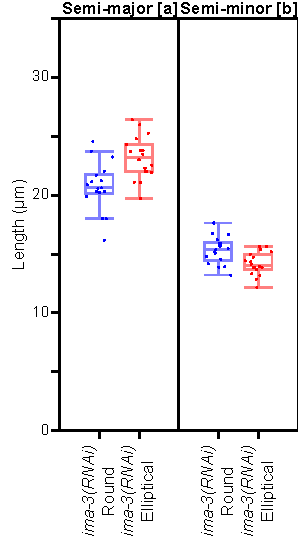
\includegraphics[width=\textwidth]{Results/FigIma3RoundElliptical/axesLength.pdf}
    \caption{Comparing embryo axes lengths. p-value = \num{7.52e-4} for semi-major axis comparison, p-value = \num{3.5e-3} for semi-minor axis comparison.} 
    \label{subfig:ima3CompareRoundElliptical-axesLength}
\end{subfigure}
\hfill
\begin{subfigure}[t]{0.3\textwidth}
    \centering
    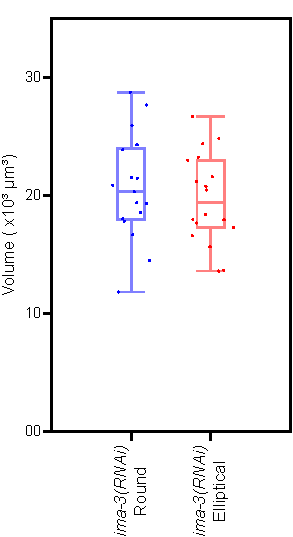
\includegraphics[width=\textwidth]{Results/FigIma3RoundElliptical/vol.pdf}
    \caption{Comparing embryo volumes. p-value = \num{0.52}.} 
    \label{subfig:ima3CompareRoundElliptical-volume}
\end{subfigure}
\hfill
\begin{subfigure}[t]{0.3\textwidth}
    \centering
    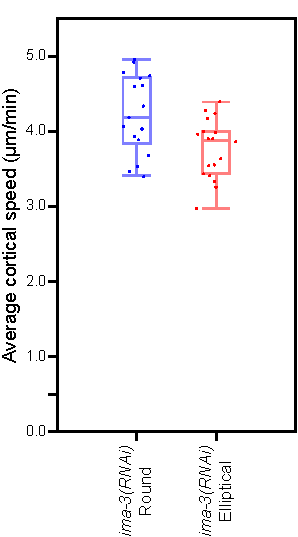
\includegraphics[width=\textwidth]{Results/FigIma3RoundElliptical/crtxSpeed.pdf}
    \caption{Comparing average cortical speeds in embryos. p-value = \num{6.3e-3}.} 
    \label{subfig:ima3CompareRoundElliptical-crtxSpeed}
\end{subfigure}
\caption[Comparing embryos between subsets of \geneExp{ima-3} \acs{rnai} embryos]{Comparing embryo geometry and cortical flow speeds between round and elliptical \geneExp{ima-3} \ac{rnai} embryos. Semi-major \longAxisLength and semi-minor \shortAxisLength axes lengths (\autoref{subfig:ima3CompareRoundElliptical-axesLength}), volume (calculated using measured semi-major and semi-minor axis lengths, \autoref{subfig:ima3CompareRoundElliptical-volume}) and average cortical flow speed (\autoref{subfig:ima3CompareRoundElliptical-crtxSpeed}) are compared. Datapoints represent axes lengths, volume and average cortical flow speed measured for individual embryos in \autoref{subfig:ima3CompareRoundElliptical-axesLength}, \autoref{subfig:ima3CompareRoundElliptical-volume} and \autoref{subfig:ima3CompareRoundElliptical-crtxSpeed} respectively. p-values are calculated using a two-sided t-test.}
\label{fig:ima3CompareRoundElliptical}
\end{figure}

\begin{figure}
\centering
\begin{subfigure}[t]{0.45\textwidth}
    \centering
    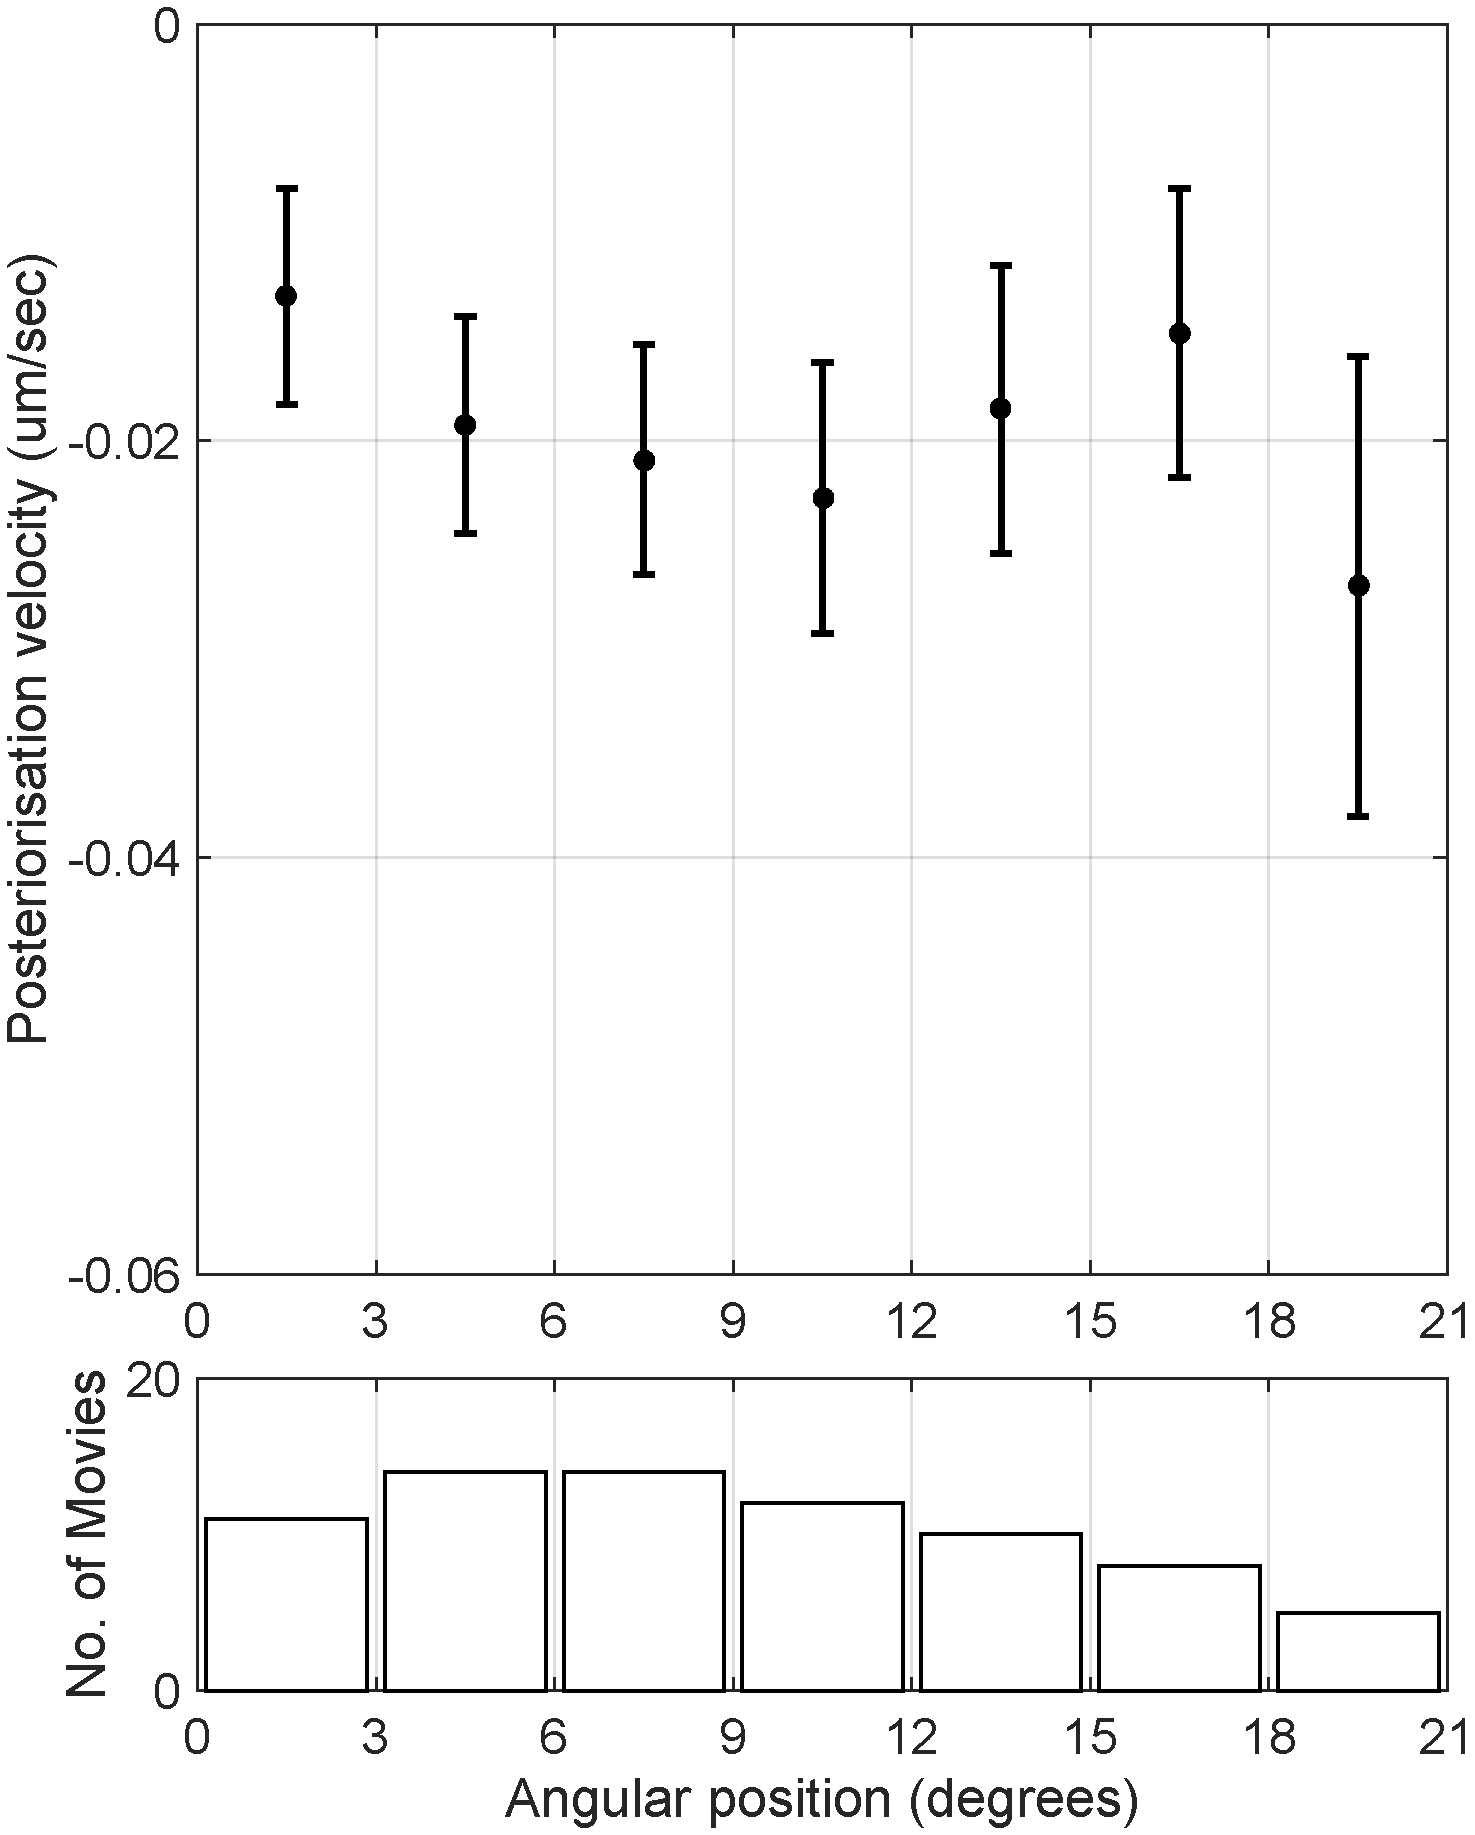
\includegraphics[width=\textwidth]{Results/FigIma3RoundElliptical/imaRound.pdf}
    \caption{Posteriorisation velocity observed in round \geneExp{ima-3} \ac{rnai} embryos} 
    \label{subfig:ima3aspRatioSplitPostVel-round}
\end{subfigure}
\hfill
\begin{subfigure}[t]{0.45\textwidth}
    \centering
    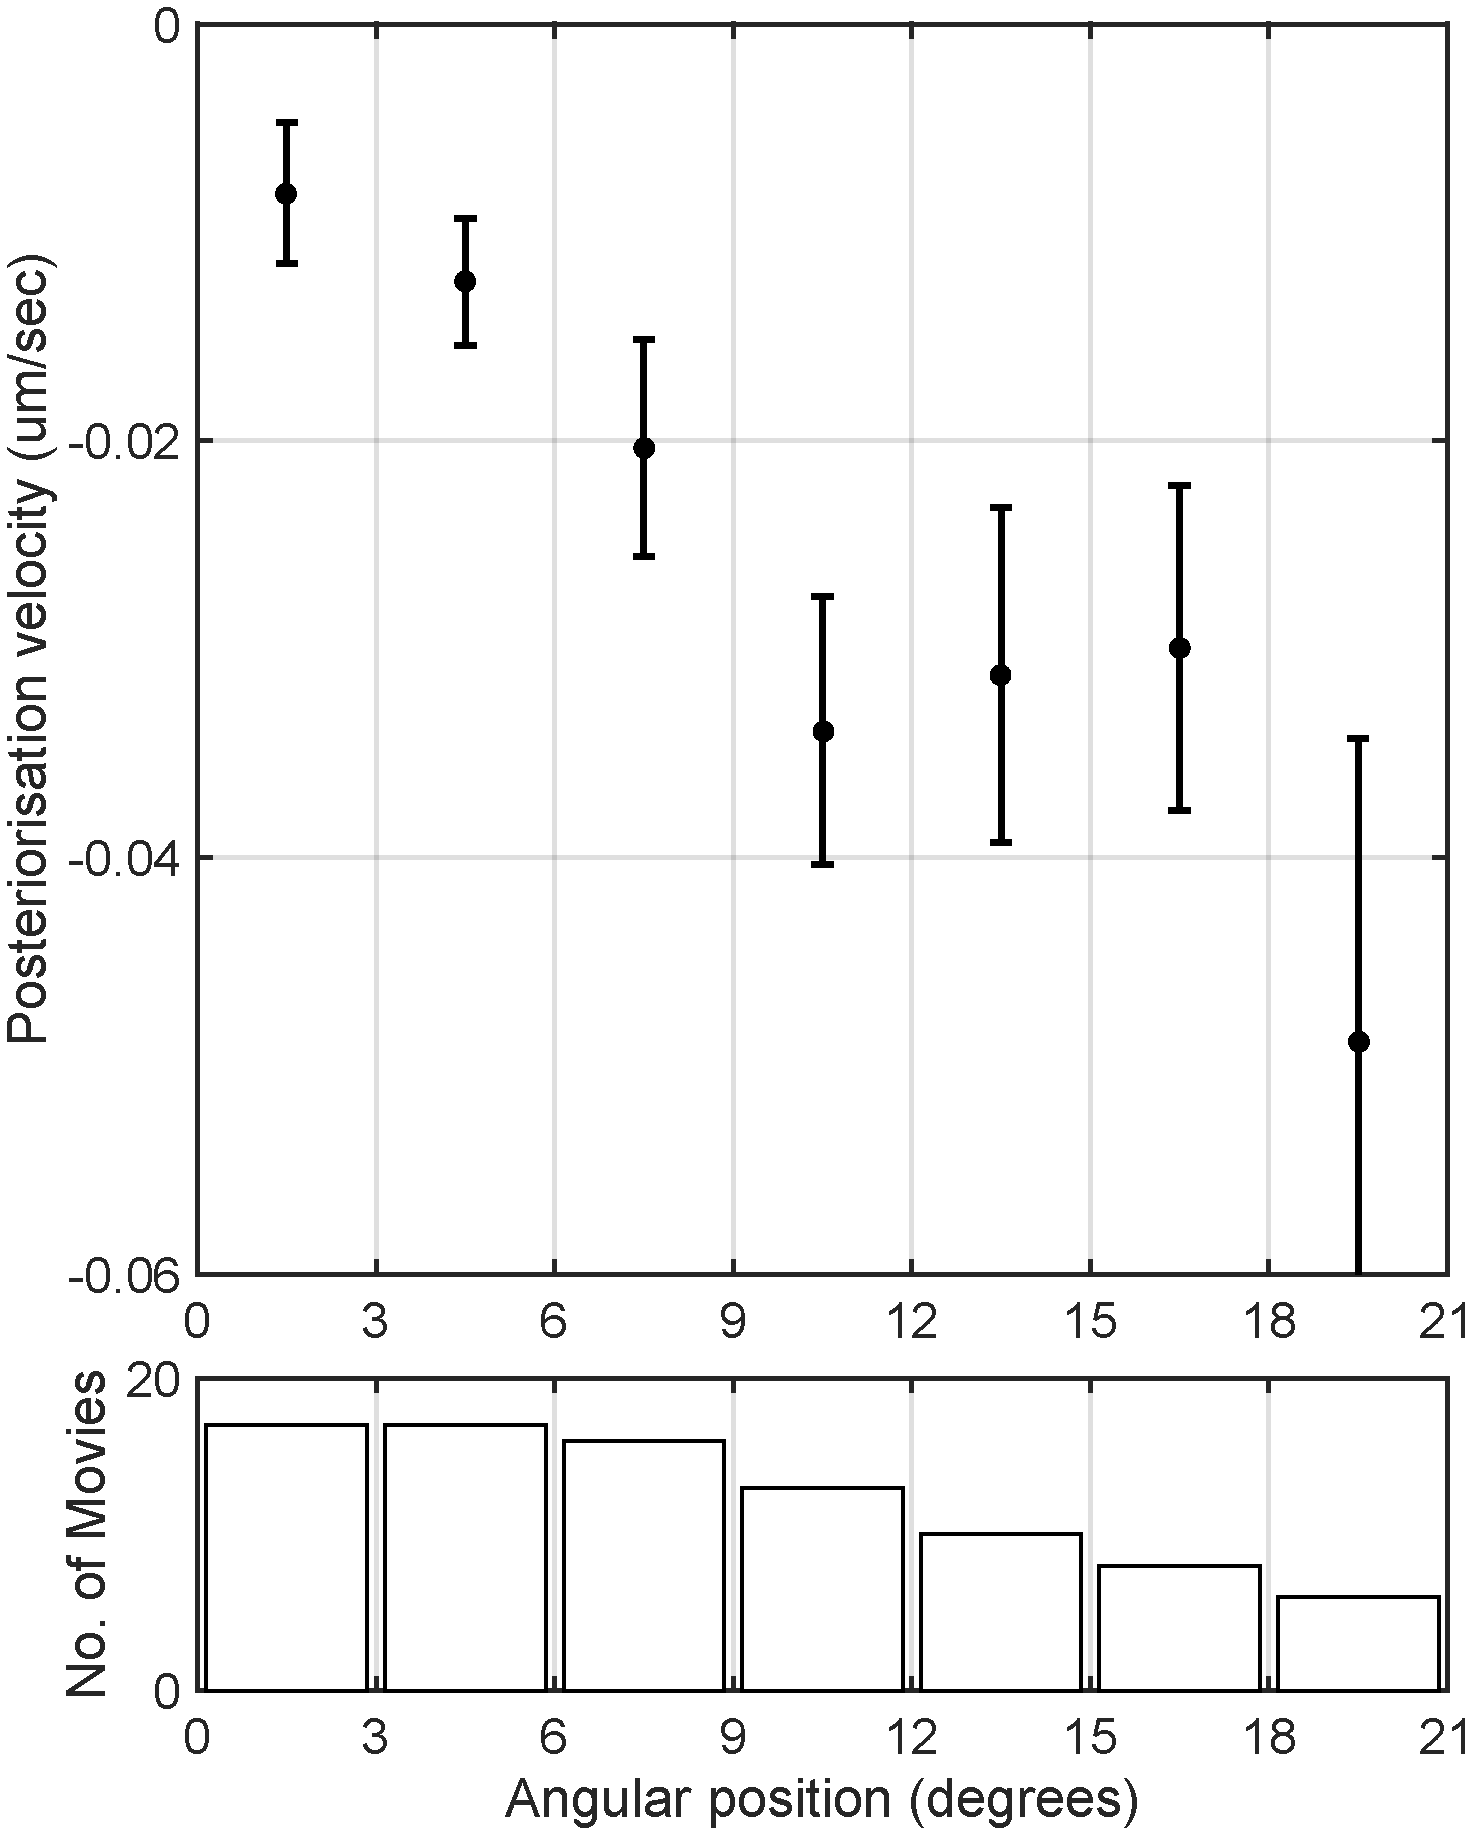
\includegraphics[width=\textwidth]{Results/FigIma3RoundElliptical/imaElliptical.pdf}
    \caption{Posteriorisation velocity observed in elliptical \geneExp{ima-3} \ac{rnai} embryos} 
    \label{subfig:ima3aspRatioSplitPostVel-ellip}
\end{subfigure}
\caption[Comparing posteriorisation of male pronucleus between subsets of \geneExp{ima-3} \acs{rnai} embryos]{Top: Posteriorization velocity of the male pronucleus (along y-axis, in \si{\unitPostVel}) plotted against its angular position, in round (N = 17, \autoref{subfig:ima3aspRatioSplitPostVel-round}) and elliptical (N = 18,\autoref{subfig:ima3aspRatioSplitPostVel-ellip}) embryos of SWG070 strain. Negative values of the posteriorisation velocity indicate movement towards the posterior end. Angular position is binned using a bin width of \SI{3}{\unitAngle}. Black circles with errors bars denote the average posteriorization velocity with \num{95}\% confidence intervals in each angular position bin. Bottom: Histogram of the number of movies (along y-axis) contributing to each angular position (along x-axis) bin. A movie is considered to contribute to an angular position bin if it has any frames with angular positions within that bin. Note that a movie can contribute to multiple bins, as it may contain frames spanning different angular positions.}
\label{fig:ima3aspRatioSplitPostVel}
\end{figure}

Altogether, these observations reconfirm the result from \autoref{subsec:roundEmbryosIma3} -- rounder embryos indeed show diminished \ac{ap} axis alignment. These observations also indicate that the relevant parameter related to embryo geometry that influences \ac{ap} axis alignment is the aspect ratio of the embryo, while differences in embryo volume may be neglected for the relation between embryo geometry and \ac{ap} axis alignment. 

%\subsubsection{\acs{ap} axis alignment in round embryos generated in \geneExp{dpy-11} mutant}\label{subsubsec:dpy11Mutant}
%In \autoref{subsec:roundEmbryosIma3}, we generated round embryos by performing a \ac{rnai} of \geneExp{ima-3}. Such round embryos can also be generated by short worms mutant in \geneExp{dpy-11} \citep{ko2002novel,yamamoto2017asymmetric}. DPY-11 is involved in the development of the cuticle of worms during post-embryonic morphogenesis, and plays an important role in the molting cycle of the worms \citep{ko2002novel}. \geneExp{dpy-11} mutant worms are shorter than unperturbed worms. In this section, we use the SWG297 strain -- a strain of worms mutant in \geneExp{dpy-11} tagged with \flurophoreLabel{\ac{nmy2}}{\ac{gfp}} and \flurophoreLabel{PHDomain}{mCherry} (see \autoref{sec:wormHandling} for details).

%Here, we describe the observed \ac{ap} axis alignment in three different sets of embryos:
%\begin{itemize}
%    \item Embryos generated from the SWG297 strain. We call these \geneExp{dpy-11} mutant embryos
%    \item Embryos generated by performed a \ac{rnai} of \geneExp{ima-3} on worms of SWG297 strain, for a feeding time of \SI{24}{\unitRNAiTime}. We call these \geneExp{ima-3} \ac{rnai}, \geneExp{dpy-11} mutant embryos.
%    \item Embryos generated by performed a double \ac{rnai} of \geneExp{ima-3} and \geneExp{mel-11} on worms of SWG297 strain, for a feeding time of \SI{24}{\unitRNAiTime}. We call these \geneExp{ima-3; mel-11} \ac{rnai}, \geneExp{dpy-11} mutant embryos.
%\end{itemize}
%We first compare cortical flows measured in the three sets. We find that average cortical flow speeds are not significantly different between the three sets: \SI{4.12 +- 0.59}{\unitCrtxVel} for \geneExp{dpy-11} mutant embryos; \SI{4.12 +- 0.59}{\unitCrtxVel} for \geneExp{ima-3} \ac{rnai}, \geneExp{dpy-11} mutant embryos; \SI{4.12 +- 0.59}{\unitCrtxVel} for \geneExp{ima-3; mel-11} \ac{rnai}, \geneExp{dpy-11} mutant embryos. Given that MEL-11 reduces the amount of myosin on the cortex (as discussed in \autoref{subsec:Nop1AndNop1Mel11}), this observation is surprising in that cortical flows are not faster in \geneExp{ima-3; mel-11} \ac{rnai}, \geneExp{dpy-11} mutant embryos. However, this could also be because of low number of embryos sampled for this set. In any case, we observe that cortical flows are similar between the three sets of embryos considered here. Note that since the cortical flows observed here are slower than those observed in unperturbed embryos or \geneExp{ima-3} \ac{rnai} embryos, a direct comparison with those sets of embryos is not feasible.

%We next compare the axes lengths and aspect ratios observed in the three sets. We observe that \geneExp{ima-3; mel-11} \ac{rnai}, \geneExp{dpy-11} mutant embryos are the most round, with average aspect ratio \aspectRatio = \num{1.2 +- 0.2} and average axes lengths \longAxisLength = \SI{10.00 +- 0.00}{\unitLength}, \shortAxisLength = \SI{10.00 +- 0.00}{\unitLength}; \geneExp{dpy-11} mutant embryos are most elliptical, with average aspect ratio \aspectRatio = \num{1.2 +- 0.2} and average axes lengths \longAxisLength = \SI{10.00 +- 0.00}{\unitLength}, \shortAxisLength = \SI{10.00 +- 0.00}{\unitLength}; and \geneExp{ima-3} \ac{rnai}, \geneExp{dpy-11} mutant embryos are in the middle, with average aspect ratio \aspectRatio = \num{1.2 +- 0.2} and average axes lengths \longAxisLength = \SI{10.00 +- 0.00}{\unitLength}, \shortAxisLength = \SI{10.00 +- 0.00}{\unitLength}. Thus, we have a gradation of aspect ratios between the three sets of embryos.

%Finally, we compare posteriorisation velocity as a function of angular positions between the three set of embryos. We find that for all angular positions, \geneExp{ima-3; mel-11} \ac{rnai}, \geneExp{dpy-11} mutant embryos exhibit the slowest posteriorisation velocity. Additionally, posteriorisation velocity is comparable between \geneExp{ima-3} \ac{rnai}, \geneExp{dpy-11}  mutant embryos and \geneExp{dpy-11}  mutant embryos, with slightly faster posteriorisation velocity observed in the latter --  upto angular position \SI{15}{\unitAngle}. Betweeen angular positions \SI{15}{\unitAngle} and \SI{21}{\unitAngle}, \geneExp{dpy-11}  mutant embryos seem to show slower posteriorisation velocity comparable to those observed in \geneExp{ima-3; mel-11} \ac{rnai}, \geneExp{dpy-11} mutant embryos. We believe this is because of the low number of embryos present in the \geneExp{dpy-11} mutant embryos set -- specifically, there is only one embryo, with aspect ratio \aspectRatio = \num{1.2}, contributing to angular position bins between \SI{15}{\unitAngle} and \SI{21}{\unitAngle} (comparable to aspect ratios observed in the \geneExp{ima-3; mel-11} \ac{rnai}, \geneExp{dpy-11} mutant embryos set).

%The observations here generally match the qualitative behaviour expected from the relation between aspect ratio and posteriorisation velocity discussed in \autoref{sec:GeometryRole}. Given the low number of embryos in each set discussed here, such a match is only indicative of the relation between embryo geometry and \ac{ap} axis alignment.

\FloatBarrier
\subsection{Are pseudocleavage furrow-dependent and cytoplasmic flow-dependent mechanisms sufficient to explain \acs{ap} axis alignment?}\label{subsec:sufficiencyTestAir1}

\subsubsection{Decoupling positions of male pronucleus and polarisation trigger via \geneExp{air-1} \ac{rnai}}\label{subsubsec:air1rnaiDecoupleMalePronucleusPolarisation}
In \autoref{sec:ApAxisEstablishment}, the mechanism of \ac{ap} axis establishment, and the role of polarisation trigger provided by the centrosomes anchored to the male pronucleus during this process, are discussed. Given this anchoring between the male pronucleus and centrosomes \citep{de2016dynein}, the position of the male pronucleus has been used in previous sections as a proxy to the position of the polarisation trigger, and thus the instantaneous orientation of the \ac{ap} axis. Here, it is investigated if this link between the position of the male pronucleus and polarisation trigger could be broken, and the effect on \ac{ap} axis alignment.

To do so, an \ac{rnai} of \geneExp{air-1} is performed on worms of SWG070 strain for a feeding time of \SI{24}{\unitRNAiTime} (see \autoref{sec:rnaiMethods} for details on \ac{rnai}). AIR-1 (or Aurora Kinase A) is a serine/theronine kinase that is essential for centrosome maturation \citep{hannak2001aurora}, among other functions related to mitotis and cytokinesis \citep{kapoor2019centrosome}. Previous studies have observed that \ac{rnai}-mediated depletion of \geneExp{air-1} leads to embryos with multiple \ac{ppar} domains instead of a single one observed in unperturbed embryos, along with two pseudocleavage furrows \citep{kapoor2019centrosome,klinkert2019aurora}. Additionally, in these \ac{rnai} embryos the centrosome is dispensible for positioning of the \ac{ap} axis \citep{kapoor2019centrosome,klinkert2019aurora}. 

\begin{figure}
\centering
\includegraphics[width=\textwidth]{Results/FigExpAir1/air1Micrograph.pdf}
\caption[Representative micrograph: \geneExp{air-1} \acs{rnai} embryos]{Representative \geneExp{air-1} \acs{rnai} embryo of SWG070 strain, labelled with \flurophoreLabel{\ac{nmy2}}{\ac{gfp}} (white), showing the 2 pseudocleavage furrows (white arrows) and 2 myosin depletion domains (white lines) that form on the anterior and posterior end. Note that the anterior and posterior myosin depletion domains form along the long axis of the embryo. Male pronucleus is indicated by white dashed circle. T = \SI{0}{\second} is set at the end of posteriorisation of the male pronucleus. Scale bar: \SI{10}{\unitLength}. Images are rotated such that anterior and posterior ends are to the left and right respectively.}
\label{fig:swg070Air1Micrograph}
\end{figure}

Observations made here in \geneExp{air-1} \ac{rnai} are found to be consistent with those made in these previous studies \citep{klinkert2019aurora,kapoor2019centrosome}. Specifically, \geneExp{air-1} \ac{rnai} embryos were observed to typically exhibit two pseudocleavage furrows, alongwith two domains where myosin is depleted -- representing the two \ac{ppar} domains. Interestingly, the two myosin depletion domains form on the opposite ends of the embryo -- that is, always aligned along the long axis of the embryo. Cortical flows observed in the \ac{rnai} embryos were found to be slower but comparable to those observed in unperturbed embryos: average cortical flow speed in \ac{rnai} embryos was measured to be \SI{3.04 +- 0.84}{\unitCrtxVel} compared to \SI{4.12 +- 0.59}{\unitCrtxVel} in unperturbed embryos -- see \autoref{fig:swg070Air1CrtxFlow}. However, no decay towards \SI{0}{\unitAngle} is observed in the angular position of the male pronucleus with time, and very slow posteriorisation velocities are observed for all angular positions -- see \autoref{fig:swg070Air1Trajectories} and \autoref{fig:swg070Air1PostVelVsAngle}. Thus, the male pronucleus does not posteriorise in the \geneExp{air-1} \ac{rnai} embryos, indicating that the \ac{rnai} embryos do not need the male pronucleus to \enquote{guide} the positioning of \ac{ppar} domain(s) (guidance here refers to centrosomes anchored to the male pronucleus -- see \cite{gross2019guiding}). This is consistent with the results of \cite{klinkert2019aurora} and \cite{kapoor2019centrosome}, which show that the centrosomes are dispensable for positioning of the \ac{ap} axis in \geneExp{air-1} \ac{rnai} embryos. However, even with no guidance from the centrosomes, polarisation in \geneExp{air-1} \ac{rnai} embryos is observe to  align with the long axis of the embryo.

\begin{table}
    \centering
    \begin{tabular}{|c|c|}
        \hline
         & No. of embryos \\
         \hline
         Polarisation aligned with long axis & \num{23}\\
         Two pseudocleavage furrows observed & \num{14}\\
         Total number of embryos & \num{23}\\
         \hline
    \end{tabular}
    \caption{Number of embryos with different features in \geneExp{air-1} \ac{rnai} embryos of SWG070 strain.}
    \label{tab:apAxisAlignmentAir1}
\end{table}

\begin{figure}
\centering
\begin{subfigure}[t]{0.4\textwidth}
    \centering
    \includegraphics[width=\textwidth]{Results/FigExpAir1/air1Tracks.pdf}
    \caption{Trajectories of the male pronucleus (denoted by the coordinates of its center) observed in \geneExp{air-1} \ac{rnai} embryos. Color represents time. x- and y-axes lie along the long and short axes of an ellipse with semi-major axis $a = \SI{28.9}{\unitLength}$ and semi-minor axis $b = \SI{15.6}{\unitLength}$. Scale bar: \SI{5}{\unitLength}} 
    \label{subfig:swg070Air1Trajectories-tracks}
\end{subfigure}
\hfill
\begin{subfigure}[t]{0.57\textwidth}
    \centering
    \includegraphics[width=\textwidth]{Results/FigExpAir1/air1Angular.pdf}
    \caption{Angular position of the male pronucleus (on y-axis, in \si{\unitAngle}) plotted as a function of time (on x-axis, in \si{\second}), in \geneExp{air-1} \ac{rnai} embryos. Black lines represent individual trajectories.} 
    \label{subfig:swg070Air1Trajectories-angleVsTime}
\end{subfigure}
\caption[Experimentally observed trajectories of the male pronucleus in \geneExp{air-1} \acs{rnai} embryos]{Experimentally observed trajectories of the male pronucleus in \geneExp{air-1} \ac{rnai} embryos of SWG070 strain (N = 23). See \autoref{subsec:nucleusTracking} for details on male pronucleus tracking. Average semi-major and semi-minor axes lengths for \geneExp{air-1} \ac{rnai} embryos of SWG070 strain are used in \autoref{subfig:swg070Air1Trajectories-tracks} -- see \autoref{tab:resultsEmbryoGeometry}. Angular position is defined as the angle between the long axis and line connecting the centers of the male pronucleus and embryo. T = \SI{0}{\second} denotes end of posteriorisation.}
\label{fig:swg070Air1Trajectories}
\end{figure}

\begin{figure}
\centering
\begin{subfigure}[t]{0.25\textwidth}
    \centering
    \includegraphics[width=\textwidth]{Results/FigExpAir1/air1CrtxSpeed.pdf}
    \caption{Comparison of average cortex flow speeds between unperturbed embryos (N = 57, blue) and \geneExp{air-1} \ac{rnai} embryos (N = 23, red), both from the SWG070 strain. Datapoints represent average cortical flow speeds measured for individual embryos.} 
    \label{subfig:swg070Air1CrtxFlow-avgSpeed}
\end{subfigure}
\hfill
\begin{subfigure}[t]{0.3\textwidth}
    \centering
    \includegraphics[width=\textwidth]{Results/FigExpAir1/crtxFlowTime.pdf}
    \caption{Average cortical flow velocity (color, in \si{\unitCrtxVel}) plotted as a function of time (along y-axis, in \si{\second}, t = \SI{0}{\second} denotes end of posteriorization) and position on the cortex (along x-axis, in \si{\unitLength}, s=\SI{0}{\unitLength} denotes posterior end), as observed in \geneExp{air-1} \ac{rnai} embryos. See \autoref{fig:resultsCorticalAvgFlowVsTime} for details and comparison.} 
    \label{subfig:swg070Air1CrtxFlow-VsTime}
\end{subfigure}
\hfill
\begin{subfigure}[t]{0.3\textwidth}
    \centering
    \includegraphics[width=\textwidth]{Results/FigExpAir1/crtxFlowAngle.pdf}
    \caption{Average cortical flow velocity (color, in \si{\unitCrtxVel}) plotted as a function of angular position of the male pronucleus (along y-axis, in \si{\unitAngle}) and position on the cortex (along x-axis, in \si{\unitLength}, s=\SI{0}{\unitLength} denotes posterior end), as observed in \geneExp{air-1} \ac{rnai} embryos. Angular positions are binned with bin width \SI{3}{\unitAngle}. See \autoref{fig:resultsCorticalAvgFlowVsAngle} for details and comparison.} 
    \label{subfig:swg070Air1CrtxFlow-VsAngle}
\end{subfigure}
\caption[Experimentally observed cortical flows in \geneExp{air-1} \acs{rnai} embryos]{Experimentally observed cortical flows in \geneExp{air-1} \ac{rnai} embryos of SWG070 strain (N = 23). See \autoref{subsec:corticalFlows} for details on measuring cortical flows.}
\label{fig:swg070Air1CrtxFlow}
\end{figure}

\begin{figure}
\centering
\includegraphics[width=0.85\textwidth]{Results/FigExpAir1/air1PostVelVsAngle.pdf}
\caption[Experimentally observed posteriorisation velocity of the male pronucleus in \geneExp{air-1} \acs{rnai} embryos]{Top: Posteriorization velocity of the male pronucleus (along y-axis, in \si{\unitPostVel}) plotted against its angular position, in \geneExp{air-1} \ac{rnai} embryos of SWG070 strain (N = 23). Negative values of the posteriorisation velocity indicate movement towards the posterior end. Angular position is binned using a bin width of \SI{3}{\unitAngle}. Black circles with errors bars denote the average posteriorization velocity with \num{95}\% confidence intervals in each angular position bin. Grey circles represent the data scatter -- the measured posteriorization velocities for different angular positions in each embryo (see \autoref{subsec:nucleusTracking}). Bottom: Histogram of the number of movies (along y-axis) contributing to each angular position (along x-axis) bin. A movie is considered to contribute to an angular position bin if it has any frames with angular positions within that bin. Note that a movie can contribute to multiple bins, as it may contain frames spanning different angular positions.}
\label{fig:swg070Air1PostVelVsAngle}
\end{figure}

In the theoretical model, the male pronucleus is advected by flows in the cytoplasm -- see \autoref{ch:ActiveMatter}. If however the male pronucleus is no longer coupled to the polarisation trigger, as seems to be case in \geneExp{air-1} \ac{rnai} embryos, then one may expect that the advection of the male pronucleus by cytoplasmic flows should have no effect on embryo polarisation. Thus, in \geneExp{air-1} \ac{rnai} embryos, cytoplasmic flow-dependent mechanism is unlikely to play a role in the alignment of the \ac{ap} axis observed in \geneExp{air-1} \ac{rnai} embryos. The pseudocleavage furrow-dependent mechanism enforces a rotation in the cortex itself, and thus should be less impacted by the broken coupling between the male pronucleus and polarisation trigger in \geneExp{air-1} \ac{rnai} embryos. Thus, \geneExp{air-1} \ac{rnai} may be a possible genetic perturbation to disable the cytoplasmic flow-dependent mechanism for \ac{ap} axis alignment.

\subsubsection{Suppressing both mechanisms via \geneExp{air-1; mel-11} \ac{rnai} in \geneExp{nop-1} mutant}
To test if the \ac{ap} axis still aligns with the long axis after both the cytoplasmic-flow dependent and pseudocleavage furrow-dependent mechanism are disabled, a double \ac{rnai} of \geneExp{air-1; mel-11} is performed on \geneExp{nop-1} mutant worms from the SWG228 strain for a feeding time of \SI{24}{\unitRNAiTime} (see \autoref{sec:rnaiMethods} for details on \ac{rnai}). This combines the two conditions we considered before: \ac{rnai} of \geneExp{air-1} to disable cytoplasmic flow-dependent mechanism, and \ac{rnai} of \geneExp{mel-11} in \geneExp{nop-1} mutant background to disable the pseudocleavage furrow-dependent mechanism. \geneExp{nop-1} mutant worms were chosen due to the difficulty in performing a triple RNAi condition and since \geneExp{nop-1} mutation is not lethal.

\begin{figure}
\centering
\includegraphics[width=\textwidth]{Results/FigExpAir1/air1mel11nop1Micrograph.pdf}
\caption[Representative micrograph: \geneExp{air-1; mel-11} \acs{rnai} in \geneExp{nop-1} mutant embryos]{Representative \geneExp{air-1; mel-11} \ac{rnai} in \geneExp{nop-1} mutant embryo of SWG228 strain, labelled with \flurophoreLabel{\ac{nmy2}}{\ac{gfp}} (white). Note the lack of pseudocleavage furrow. White arrows indicate the myosin depletion domain (indicating the \ac{ppar} domain) which initiates away from the male pronucleus. Note that this domain is not along the long axis of the embryo. Scale bar: \SI{10}{\unitLength}. Images are rotated such that anterior and posterior ends are to the left and right respectively.}
\label{fig:swg228Air1Nop1Mel11Micrograph}
\end{figure}

As expected from observations in \geneExp{nop-1; mel-11} \ac{rnai} embryos, no pseudocleavage furrows are observed in \geneExp{air-1; mel-11} \ac{rnai} in \geneExp{nop-1} mutant embryos (\num{13} out of \num{13} embryos). However, the domain where myosin is depleted (indicating the \ac{ppar} domain) is observed to not re-align back towards the tip of the embryo (\num{6} out of \num{13} embryos), in the few embryos that start with a myosin depletion domain away from the poles of the embryos (\num{7} out of \num{13} embryos) -- see \autoref{tab:noApAxisAlignmentAir1Nop1Mel11}. These preliminary experiments seem to suggest that \ac{ap} axis alignment is heavily suppressed in \geneExp{air-1; mel-11} \ac{rnai} in \geneExp{nop-1} mutant embryos -- however, additional experimental data are needed for a conclusive result.

\begin{table}
    \centering
    \begin{tabular}{|c|c|}
        \hline
         & No. of embryos \\
         \hline
         Myosin depletion domain starts away from poles & \num{7}\\
         \ac{ap} axis alignment fails & \num{6}\\
         Total number of embryos & \num{13}\\
         \hline
    \end{tabular}
    \caption{\ac{ap} axis alignment in \geneExp{air-1; mel-11} \ac{rnai} in \geneExp{nop-1} mutant embryos of SWG228 strain.}
    \label{tab:noApAxisAlignmentAir1Nop1Mel11}
\end{table}

\FloatBarrier
\subsection{Role of microtubules in \acs{ap} axis alignment}\label{subsec:MicrotubuleRoleGoa1Gpa16}
In \autoref{sec:ApAxisEstablishment}, the mechanism of \ac{ap} axis establishment is discussed, including the polarity trigger provided by the centrosomes associated with the male pronucleus that initiate \ac{ap} axis establishment. Microtubule asters emanating from these centrosomes play a key role in the \ac{ap} axis establishment process, by protecting the nascent \ac{ppar} domain that forms on the cortex near the male pronucleus \citep{wallenfang2000polarization,gross2019guiding}. In the investigation of the mechanism(s) driving \ac{ap} axis alignment so far, any role of the astral microtubules emanating from the centrosomes have been neglected. A possible way in which these microtubules could influence the posteriorisation of the male pronucleus is via forces generated by dynein motors anchored at the cortex that pull on the astral microtubules abutting the cortex. As discussed in \autoref{subsec:ComponentsCytoskeleton}, dynein motors are one of two families of motor proteins that bind to microtubules. They are (-)-end directed motor proteins \citep{de2016dynein}. Previous studies have explored the role of dynein motors in the positioning of centrosomes. Especially, dynein motors anchored to the cortex have been found to be influential in positioning the mitotic spindle, by pulling onto astral microtubules \citep{de2016dynein,gotta2001distinct,nguyen2007coupling,colombo2003translation}. Here, it is investigated if such pulling forces generated at the cortex by cortical dynein motors could influence the posteriorisation of the male pronucleus observed during \ac{ap} axis alignment.

In this subsection, embryos from the SWG057 strain are used -- instead of the SWG070 strain that has been used so far. SWG057 strain is labelled with \flurophoreLabel{\ac{tub}}{\ac{gfp}} -- which labels tubulin monomers that form the microtubules -- and \flurophoreLabel{\ac{nmy2}}{mKate}. Thus this strain allows visualisation of both the microtubules and the centrosomes, and cortical myosin -- while still allowing tracking of the position of the male pronucleus as a dark circle in the myosin channel -- see \autoref{sec:imageAnalysis} for details on how movies generated with embryos from SWG057 were analysed. As with the SWG070, time-lapse microscopy movies of one-cell stage embryos generated from SWG057 strain were taken -- see \autoref{sec:microscope} for details on microscopy. 

\begin{figure}
\centering
\includegraphics[width=\textwidth]{Results/FigExpGoa1Gpa16/wtMicrograph.pdf}
\caption[Representative micrograph: unperturbed embryos of SWG057 strain]{Representative unperturbed embryo of SWG057 strain, labelled with \flurophoreLabel{\ac{nmy2}}{mKate} (top) and \flurophoreLabel{\ac{tub}}{\ac{gfp}} (bottom), showing the posteriorisation of the male pronucleus. Bottom: White arrow indicates centrosomes, yellow arrow indicates the separation of centrosomes during pronuclear meeting. Scale bar: \SI{10}{\unitLength}. Images are rotated such that anterior and posterior ends are to the left and right respectively.}
\label{fig:swg057WtMicrograph}
\end{figure}

\begin{figure}
\centering
\begin{subfigure}[t]{0.45\textwidth}
    \centering
    \includegraphics[width=\textwidth]{Results/FigExpGoa1Gpa16/wt_corticalflow_timeFig.pdf}
    \caption{Average cortical flow velocity (color, in \si{\unitCrtxVel}) plotted as a function of time (along y-axis, in \si{\second}, t = \SI{0}{\second} denotes end of posteriorization) and position on the cortex (along x-axis, in \si{\unitLength}, s=\SI{0}{\unitLength} denotes posterior end), as observed in unperturbed embryos of SWG057 strain. See \autoref{fig:resultsCorticalAvgFlowVsTime} for details and comparison.} 
    \label{subfig:swg057WtCrtxFlow-VsTime}
\end{subfigure}
\hfill
\begin{subfigure}[t]{0.45\textwidth}
    \centering
    \includegraphics[width=\textwidth]{Results/FigExpGoa1Gpa16/wt_corticalflow_angleFig.pdf}
    \caption{Average cortical flow velocity (color, in \si{\unitCrtxVel}) plotted as a function of angular position of the male pronucleus (along y-axis, in \si{\unitAngle}) and position on the cortex (along x-axis, in \si{\unitLength}, s=\SI{0}{\unitLength} denotes posterior end), as observed in unperturbed embryos of SWG057 strain. Angular positions are binned with bin width \SI{3}{\unitAngle}. See \autoref{fig:resultsCorticalAvgFlowVsAngle} for details and comparison.} 
    \label{subfig:swg057WtCrtxFlow-VsAngle}
\end{subfigure}
\caption[Experimentally observed cortical flows in unperturbed SWG057 embryos]{Experimentally observed cortical flows in unperturbed embryos of SWG057 strain (N = 32). See \autoref{subsec:corticalFlows} for details on measuring cortical flows.}
\label{fig:swg057WtCrtxFlow}
\end{figure}

The rate of \ac{ap} axis alignment in unperturbed embryos of the SWG057 strain is characeterised by measuring the posteriorisation velocity of the male pronucleus as a function of angular position of the male pronucleus in these embryos. In unperturbed embryos, the male pronucleus is observed to move, on average, towards the posterior end -- with faster posteriorisation velocity at higher angular positions  -- see \autoref{subfig:compareWtGoa1Gpa16PostVel-wt}. Cortical flows in unperturbed embryos from SWG057 strain were also measured -- see \autoref{sec:imageAnalysis} for methods -- yielding an average cortical speed of \SI{2.84 +- 0.37}{\unitCrtxVel} for the unperturbed embryos of SWG057 strain -- see \autoref{fig:swg057WtCrtxFlow}. Observed cortical flows are binned using angular positions of the male pronucleus -- see \autoref{sec:statAnalysis}. The point where the cortical flows change sign is observed to correlate with the angular position. Given that these observations are similar to those made for the unperturbed embryos from the SWG070 strain (see \autoref{sec:apAxisAlignCharacteriseWT}), it is concluded that the unperturbed embryos from SWG057 exhibit similar \ac{ap} axis alignment characteristics as compared to unperturbed embryos from SWG070. Note however that the cortical flows observed in unperturbed embryos of the SWG057 strain are slower compared to those observed in the unperturbed embryos of the SWG070 strain.

To test if cortically anchored dynein motors pulling on astral microtubules influence \ac{ap} axis alignment, the proteins that anchor the dynein motors to the cortex are suppressed. Specifically, a double \ac{rnai} of \geneExp{goa-1} and \geneExp{gpa-16} is performed on worms of SWG057 strain for a feeding time of \SI{24}{\unitRNAiTime} (see \autoref{sec:rnaiMethods} for details on double \ac{rnai}). GOA-1 and GPA-16 are heterotrimeric G$\alpha$ proteins that, along with GPR-1/2 and LIN-5, help anchor dynein at the cortex \citep{de2016dynein,nguyen2007coupling,colombo2003translation}. Thus, their reduction via the double \ac{rnai} leads to depletion of cortically anchored dynein motors \citep{de2016dynein}. Cortical flows measured in \geneExp{goa-1; gpa-16} \ac{rnai} embryos are compared with those observed in unperturbed embryos, both of the SWG057 strain. On comparison, the cortical flows in the two sets of embryos are found to not be significantly different, with a measured average cortical speed of \SI{2.62 +- 0.52}{\unitCrtxVel} in \geneExp{goa-1; gpa-16} \ac{rnai} embryos compared to \SI{2.84 +- 0.37}{\unitCrtxVel} in unperturbed embryos -- see \autoref{fig:swg057Goa1Gpa16CrtxFlow}. Finally, the posteriorisation velocity observed in \geneExp{goa-1; gpa-16} \ac{rnai} embryos are compared to those observed in unperturbed embryos, for different angular positions -- finding not much difference between the two, for all angular positions considered (\SIrange{0}{21}{\unitAngle}), and therefore implying that the posteriorisation of the male pronucleus does not differ significantly between \geneExp{goa-1; gpa-16} \ac{rnai} embryos and unperturbed embryos -- see \autoref{fig:compareWtGoa1Gpa16PostVel}. These observations indicate that the double \ac{rnai} \geneExp{goa-1; gpa-16} does not significantly affect either the cortical flow or the posteriorisation of the male pronucleus. Altogether, these observations lead to the conclusion that the forces generated by cortical dynein as they pull on astral microtubule do not play an significant role in \ac{ap} axis alignment.

\begin{figure}
\centering
\includegraphics[width=\textwidth]{Results/FigExpGoa1Gpa16/goa1gpa16Micrograph.pdf}
\caption[Representative micrograph: \geneExp{goa-1; gpa-16} \acs{rnai} embryos of SWG057 strain]{Representative \geneExp{goa-1; gpa-16} \acs{rnai} embryo of SWG057 strain, labelled with \flurophoreLabel{\ac{nmy2}}{mKate} (top) and \flurophoreLabel{\ac{tub}}{\ac{gfp}} (bottom), showing the posteriorisation of the male pronucleus. Bottom: White arrow indicates centrosomes, yellow arrow indicates the separation of centrosomes during pronuclear meeting. Compare to \autoref{fig:swg057WtMicrograph} -- \geneExp{goa-1; gpa-16} \ac{rnai} embryos exhibit smaller separation between centrosomes \citep{de2016dynein}. Scale bar: \SI{10}{\unitLength}. Images are rotated such that anterior and posterior ends are to the left and right respectively.}
\label{fig:swg057Goa1Gpa16Micrograph}
\end{figure}

\begin{figure}
\centering
\begin{subfigure}[t]{0.25\textwidth}
    \centering
    \includegraphics[width=\textwidth]{Results/FigExpGoa1Gpa16/avgCrtxSpeed.pdf}
    \caption{Comparison of average cortex flow speeds between unperturbed embryos (N = 32, blue) and \geneExp{goa-1; gpa-16} \ac{rnai} embryos (N = 30, red), both from the SWG057 strain. Datapoints represent average cortical flow speeds measured for individual embryos.} 
    \label{subfig:swg057Goa1Gpa16CrtxFlow-avgSpeed}
\end{subfigure}
\hfill
\begin{subfigure}[t]{0.3\textwidth}
    \centering
    \includegraphics[width=\textwidth]{Results/FigExpGoa1Gpa16/goa1gpa16_corticalflow_timeFig.pdf}
    \caption{Average cortical flow velocity (color, in \si{\unitCrtxVel}) plotted as a function of time (along y-axis, in \si{\second}, t = \SI{0}{\second} denotes end of posteriorization) and position on the cortex (along x-axis, in \si{\unitLength}, s=\SI{0}{\unitLength} denotes posterior end), as observed in \geneExp{goa-1; gpa-16} \ac{rnai} embryos of SWG057 strain. See \autoref{fig:resultsCorticalAvgFlowVsTime} for details and comparison.} 
    \label{subfig:swg057Goa1Gpa16CrtxFlow-VsTime}
\end{subfigure}
\hfill
\begin{subfigure}[t]{0.3\textwidth}
    \centering
    \includegraphics[width=\textwidth]{Results/FigExpGoa1Gpa16/goa1gpa16_corticalflow_angleFig.pdf}
    \caption{Average cortical flow velocity (color, in \si{\unitCrtxVel}) plotted as a function of angular position of the male pronucleus (along y-axis, in \si{\unitAngle}) and position on the cortex (along x-axis, in \si{\unitLength}, s=\SI{0}{\unitLength} denotes posterior end), as observed in \geneExp{goa-1; gpa-16} \ac{rnai} embryos of SWG057 strain. Angular positions are binned with bin width \SI{3}{\unitAngle}. See \autoref{fig:resultsCorticalAvgFlowVsAngle} for details and comparison.} 
    \label{subfig:swg057Goa1Gpa16CrtxFlow-VsAngle}
\end{subfigure}
\caption[Experimentally observed cortical flows in \geneExp{goa-1; gpa-16} \acs{rnai} SWG057 embryos]{Experimentally observed cortical flows in \geneExp{goa-1; gpa-16} \ac{rnai} embryos of SWG057 strain (N = 30). See \autoref{subsec:corticalFlows} for details on measuring cortical flows. p-value = \num{0.14} for comparison between average cortical flow speeds in \autoref{subfig:swg057Goa1Gpa16CrtxFlow-avgSpeed}, after removing outliers. p-value calculated via a two-sided t-test.}
\label{fig:swg057Goa1Gpa16CrtxFlow}
\end{figure}

\begin{figure}
\centering
\begin{subfigure}[t]{0.45\textwidth}
    \centering
    \includegraphics[width=\textwidth]{Results/FigExpGoa1Gpa16/wtPostVel.pdf}
    \caption{Posteriorisation velocity observed in unperturbed embryos of SWG057 strain} 
    \label{subfig:compareWtGoa1Gpa16PostVel-wt}
\end{subfigure}
\hfill
\begin{subfigure}[t]{0.45\textwidth}
    \centering
    \includegraphics[width=\textwidth]{Results/FigExpGoa1Gpa16/goa1gpa16PostVel.pdf}
    \caption{Posteriorisation velocity observed in \geneExp{goa-1; gpa-16} \ac{rnai} embryos of SWG057 strain} 
    \label{subfig:compareWtGoa1Gpa16PostVel-goa1gpa16}
\end{subfigure}
\caption[Comparing posteriorisation of male pronucleus between unperturbed and \geneExp{goa-1; gpa-16} \acs{rnai} embryos of SWG057 strain]{Top: Posteriorization velocity of the male pronucleus (along y-axis, in \si{\unitPostVel}) plotted against its angular position, in unperturbed (N = 32, \autoref{subfig:compareWtGoa1Gpa16PostVel-wt}) and \geneExp{goa-1; gpa-16} \ac{rnai} (N = 30,\autoref{subfig:compareWtGoa1Gpa16PostVel-goa1gpa16}) embryos of SWG057 strain. Negative values of the posteriorisation velocity indicate movement towards the posterior end. Angular position is binned using a bin width of \SI{3}{\unitAngle}. Black circles with errors bars denote the average posteriorization velocity with \num{95}\% confidence intervals in each angular position bin. Black circles represent the data scatter -- the measured posteriorization velocities for different angular positions in each embryo (see \autoref{subsec:nucleusTracking}). Bottom: Histogram of the number of movies (along y-axis) contributing to each angular position (along x-axis) bin. A movie is considered to contribute to an angular position bin if it has any frames with angular positions within that bin. Note that a movie can contribute to multiple bins, as it may contain frames spanning different angular positions. Data only available until \SI{21}{\unitAngle} for \geneExp{goa-1; gpa-16} \ac{rnai} embryos.}
\label{fig:compareWtGoa1Gpa16PostVel}
\end{figure}

%\begin{figure}[p]
%\centering
%\begin{subfigure}[t]{0.47\textwidth}
%    \centering
%    \includegraphics[width=\textwidth]{Results/FigExpUnperturbed/wtCorticalFlowsVsTime.pdf}
%    \caption{Average cortical flows (see colorbar in \autoref{subfig:swg070WtCorticalFlowsExperiments-schematic}) plotted as a function position on the cortex (along x-axis, in \si{\unitLength}, measured along the contour of the embryo boundary) and time relative to end of posteriorisation (along y-axis, in \si{\second}, t = \SI{0}{\second} denotes end of posteriorisation). Average cortical flow velocity at a given time and position is obtained by averaging over all angular positions and all embryos.} 
%    \label{subfig:swg070WtCorticalFlowsExperiments-vsTime}
%\end{subfigure}
%\hfill
%\begin{subfigure}[t]{0.47\textwidth}
%    \centering
%    \includegraphics[width=\textwidth]{Results/FigExpUnperturbed/wtCorticalFlowsVsAngle.pdf}
%    \caption{Average cortical flows (see colorbar in \autoref{subfig:swg070WtCorticalFlowsExperiments-schematic}) plotted as a function position on the cortex (along x-axis, in \si{\unitLength}, measured along the contour of the embryo boundary) and angular position of the male pronucleus (along y-axis, in \si{\unitAngle}). Average cortical flow velocity at a given time and angular position bin (of bin width \SI{3}{\unitAngle}) of the male pronucleus is obtained by averaging over all frames in all embryos that have angular positions in said angular position bin. Dashed black line indicates the correlation between the point where the cortical flows change sign and the angular position.} 
%    \label{subfig:swg070WtCorticalFlowsExperiments-vsAngle}
%\end{subfigure}
%\hfill
%\begin{subfigure}{\textwidth}
%    \centering
%    \includegraphics[width=0.5\textwidth]{Results/corticalFlowDefine.pdf}
%    \caption{Schematic. $s$ represents the Distance from the posterior end (denoted as $s = 0$) along the cortex, with distances in the anti-clockwise direction considered positive -- this is used as the x-axis of the plots in \autoref{subfig:swg070WtCorticalFlowsExperiments-vsTime} and \autoref{subfig:swg070WtCorticalFlowsExperiments-vsAngle}. Color bar maps the colors in the plots to cortical velocity in \si{\unitCrtxVel}. Red shades indicates cortical flow pointing in the anti-clockwise direction (i.e. along the increasing direction of $s$, denoted as positive flow velocity), and blue shades in the clockwise direction (denoted as negative flow velocity). $\alpha$ represents the angular position of the male pronucleus.} 
%    \label{subfig:swg070WtCorticalFlowsExperiments-schematic}
%\end{subfigure}
%\caption[Observed cortical flows in unperturbed embryos]{Experimentally measured average cortical flow velocity in unperturbed embryos of SWG070 strain  (N = 57), plotted as a function position on the cortex (along x-axis, in \si{\unitLength}, measured along the contour of the embryo boundary) and time relative to end of posteriorisation (\autoref{subfig:swg070WtCorticalFlowsExperiments-vsTime}) or angular position of the male pronucleus (\autoref{subfig:swg070WtCorticalFlowsExperiments-vsAngle}). Cortical flow velocities are color-coded according to their magnitude and direction (\autoref{subfig:swg070WtCorticalFlowsExperiments-schematic}). See \autoref{subsec:corticalFlows} for details on measuring cortical flows from microscopy movies, and \autoref{sec:statAnalysis} on details on calculating average cortical flows.}
%\label{fig:swg070WtCorticalFlowsExperiments}
%\end{figure}